\documentclass[11pt]{report}

\usepackage[bookmarks=true,bookmarksopen=true]{hyperref}
\usepackage{url}
\usepackage{datetime}
\usepackage{proof}
\usepackage{enumerate}
\usepackage{graphicx}
\usepackage{proof}
\usepackage[backgroundcolor=white,linecolor=black]{todonotes}
\usepackage{tocbibind}


% \usepackage{setspace}
% \doublespacing

\synctex=1

%!TEX root = dissertation.tex

\usepackage{amsmath,amssymb,amsthm}
\usepackage{bcprules}
\usepackage{graphicx}
\usepackage{stmaryrd}
\usepackage{nicefrac}

\theoremstyle{plain}
\newtheorem{lemma}{Lemma}
\newtheorem{theorem}{Theorem}
\newtheorem{corollary}{Corollary}
\newtheorem{proposition}{Proposition}
\newtheorem{conjecture}{Conjecture}

\theoremstyle{definition}
\newtheorem{definition}{Definition}

\theoremstyle{remark}
\newtheorem{note}{Note}
\newtheorem*{remark}{Remark}


\newcommand{\bnfbar}{\ensuremath{~|~}}
\newcommand{\bnfdef}{\ensuremath{~::=~}}

%% set notation
\newcommand{\set}[1]{\left\lbrace #1 \right\rbrace}
\newcommand{\setof}[2]{\set{#1 \mid #2}}
\newcommand{\bigset}[1]{\left\lbrace #1 \right\rbrace}
\newcommand{\bigsetof}[2]{\bigset{#1 \mid #2}}

\DeclareMathOperator{\funcompat}{\smile}

\newcommand{\mtab}{\ensuremath{\;\;\;}}

\newcommand{\powerset}[1]{\ensuremath{\mathcal{P}(#1)}}
\newcommand{\zorch}{\ensuremath{\lightning}}

\DeclareMathOperator{\opdom}{\mathrm{dom}}
\newcommand{\dom}[1]{\ensuremath{\opdom(#1)}}

\newcommand{\bvt}{\ensuremath{\mathbf{t}}}
\newcommand{\bvf}{\ensuremath{\mathbf{f}}}

\newcommand{\llen}[1]{\ensuremath{|#1|}}
\newcommand{\lsingle}[1]{\ensuremath{\left[#1\right]}}
\newcommand{\lnil}[0]{\ensuremath{\epsilon}}
\newcommand{\elems}[1]{\ensuremath{|\!|#1|\!|}}
\newcommand{\funof}[1]{\ensuremath{\overline{#1}}}
\DeclareMathOperator{\lapp}{+\!\!\!+}
\DeclareMathOperator{\lcons}{:\!:}
\newcommand{\lhead}[1]{\ensuremath{\mathit{hd}(#1)}}
\newcommand{\ltail}[1]{\ensuremath{\mathit{tl}(#1)}}
\newcommand{\nth}[2]{\ensuremath{#2 ! #1}}
\newcommand{\listof}[1]{\ensuremath{#1~\mathsf{list}}}

\newcommand{\relset}[1]{\ensuremath{|#1|}}
\newcommand{\ext}[1]{\ensuremath{\hat{#1}}}
\newcommand{\restrict}[2]{\ensuremath{#1 |_{#2}}}
\newcommand{\proj}[2]{\ensuremath{#1 |_{#2}}}

\newcommand{\reclit}[1]{\ensuremath{\set{#1}}}

\DeclareMathOperator{\tfun}{\rightarrow}
\DeclareMathOperator{\pfun}{\rightharpoonup}
\DeclareMathOperator{\fpfun}{\pfun_{\mathrm{fin}}}

\DeclareMathOperator{\st}{\,:\,}

\newcommand{\ptup}[2]{\ensuremath{#1 \shortleftarrow #2}}
\newcommand{\funup}[2]{\ensuremath{#1 \left[ #2 \right]}}
\newcommand{\fundel}[2]{\ensuremath{#1 \setminus#2 }}
\newcommand{\recup}[3]{\funup{#1}{\ptup{#2}{#3}}}
\newcommand{\ptapp}[2]{\ensuremath{#1 \lapp #2}}

\DeclareMathOperator{\conj}{\,\wedge\,}
\DeclareMathOperator{\disj}{\,\vee\,}
\DeclareMathOperator{\onlyif}{\,\Rightarrow\,}
%\DeclareMathOperator{\ifandonlyif}{\,\Longleftrightarrow\,}
\renewcommand{\iff}{\ensuremath{\Leftrightarrow}}

\newcommand{\fresh}[1]{\ensuremath{\mathrm{fresh}(#1)}}
\newcommand{\subst}[2]{\ensuremath{\left[#1 / #2\right]}}
\newcommand{\unsubst}[2]{\ensuremath{\left[#1 \backslash #2\right]}}

\newcommand{\eqclass}[1]{\ensuremath{\left[ #1 \right]}}
\DeclareMathOperator{\downop}{\downarrow}
\newcommand{\downo}[2]{\ensuremath{\downop_{#1}\!#2}}
\newcommand{\down}[1]{\ensuremath{\downop\!#1}}

%% Calculational proofs

\newcommand{\Calc}[1]{\begin{description}
                \item \begin{tabbing}\qquad\=\quad\=\kill
                \> \> #1\end{tabbing}
                \end{description}}
\newcommand{\conn}[2]{\\*$#1 $\> \{#2\}\\\> \>}
\newcommand{\Conn}[1]{\conn{=}{#1}}

\newcommand{\ident}[1]{\ensuremath{\mathit{Id}_{#1}}}
\DeclareMathOperator{\rcomp}{\circ}
\newcommand{\relexp}[2]{\ensuremath{\stackrel{#2}{#1}}}
\newcommand{\tcl}[1]{\stackrel{+}{#1}}
\newcommand{\rtcl}[1]{\stackrel{\ast}{#1}}

\newcommand{\image}[2]{\ensuremath{#1\left[#2\right]}}
\newcommand{\invimage}[2]{\ensuremath{#1^{-1}\left[#2\right]}}

\newcommand{\lift}[1]{\ensuremath{\mathit{lift}_{#1}}}
\renewcommand{\merge}{\ensuremath{\uplus}}

% \newcommand{\override}{\reflectbox{\rotatebox[origin=c]{180}{\ensuremath{\,\oslash\,}}}}
\newcommand{\override}{\ensuremath{\backslash\!\!\backslash}}

\newcommand{\sentails}{\ensuremath{\,\models\,}}
\newcommand{\satisfies}{\ensuremath{\,\models\,}}
\newcommand{\sequiv}{\ensuremath{\,\equiv\,}}

\newcommand{\fixme}[1]{\todo{FIXME: #1}}

\DeclareMathOperator{\eqdef}{\;=_{\mathit{df}}\;}
\DeclareMathOperator{\iffdef}{\;\equiv_{\mathit{df}}\;}

\newcommand{\card}[1]{\left|#1\right|}
\newcommand{\cmpl}[1]{\ensuremath{\overline{#1}}}

\newcommand{\refines}{\ensuremath{\sqsubseteq}}
%!TEX root = dissertation.tex

\usepackage{stackrel}

%% types

\newcommand{\setlocations}{\ensuremath{\mathbb{L}}}
\newcommand{\setvalues}{\ensuremath{\mathbb{V}}}
\newcommand{\setintegers}{\ensuremath{\mathbb{Z}}}
\newcommand{\setnaturals}{\ensuremath{\mathbb{N}}}
\newcommand{\setpositives}{\ensuremath{\mathbb{N}^+}}
\newcommand{\setidentifiers}{\ensuremath{\mathbb{I}}}
\newcommand{\setbooleans}{\ensuremath{\mathbb{B}}}
\newcommand{\setprocessors}{\ensuremath{\mathbb{P}}}

\newcommand{\setevents}{\ensuremath{\mathbb{E}}}
\newcommand{\proc}[1]{\ensuremath{\mathit{proc}(#1)}}
\newcommand{\eqproc}{\ensuremath{\approx}}
\newcommand{\tp}[1]{\ensuremath{\mathit{type}(#1)}}
\newcommand{\tpflush}{\ensuremath{\mathtt{flush}}}
\newcommand{\tpwrite}[1]{\ensuremath{\mathtt{write}(#1)}}
\newcommand{\tpalloc}[1]{\ensuremath{\mathtt{alloc}(#1)}}
\newcommand{\writesto}[1]{\ensuremath{\mathit{Wr}_{#1}}}
\newcommand{\allocs}[1]{\ensuremath{\mathit{Al}_{#1}}}
\newcommand{\writes}{\ensuremath{\mathit{Wr}}}
\newcommand{\flushes}{\ensuremath{\mathit{Fl}}}


%% abbreviations
\newcommand{\setstores}{\ensuremath{\mathbf{Store}}}
\newcommand{\setstacks}{\ensuremath{\mathbf{Stack}}}
\newcommand{\setheaps}{\ensuremath{\mathbf{Heap}}}
\newcommand{\setbuffers}{\ensuremath{\mathbf{Buf}}}
\newcommand{\setshares}{\ensuremath{\mathbf{Share}}}
\newcommand{\setperms}{\ensuremath{\mathbf{Perm}}}
\newcommand{\setastates}{\ensuremath{\mathit{\Sigma}}}
\newcommand{\setstates}{\ensuremath{\mathbf{State}}}
\newcommand{\setpstates}{\ensuremath{\Pi}}
\newcommand{\setmpstates}{\ensuremath{\mathbf{MPState}}}
\newcommand{\setresolvers}{\ensuremath{\mathbf{Resolver}}}
\newcommand{\setconfigurations}{\ensuremath{\mathbf{Config}}}
\newcommand{\setmconfigurations}{\ensuremath{\mathbf{MConfig}}}
\newcommand{\setassertions}{\ensuremath{\mathbf{Assert}}}

%% operators 

\DeclareMathOperator{\op}{\mathit{op}}
\DeclareMathOperator{\opskip}{\mathsf{skip}}
\DeclareMathOperator{\opfence}{\mathsf{fence}}
\DeclareMathOperator{\opassume}{\mathsf{assume}}
\DeclareMathOperator{\opassert}{\mathsf{assert}}
\DeclareMathOperator{\opassign}{:\!=}
\DeclareMathOperator{\opequals}{=}
\DeclareMathOperator{\opseq}{;}
\DeclareMathOperator{\opchoice}{+}
\DeclareMathOperator{\oppar}{||}
\DeclareMathOperator{\oploop}{\ast}
\DeclareMathOperator{\oplock}{\mathsf{lock}}
\DeclareMathOperator{\opunlock}{\mathsf{unlock}}
\DeclareMathOperator{\opcons}{\mathsf{cons}}
\DeclareMathOperator{\opnew}{\mathsf{new}}
\DeclareMathOperator{\opalloc}{\mathsf{alloc}}
\DeclareMathOperator{\opdispose}{\mathsf{free}}
\DeclareMathOperator{\opif}{\mathsf{if\,}}
\DeclareMathOperator{\opthen}{\mathsf{\,then\,}}
\DeclareMathOperator{\opelse}{\mathsf{\,else}}
\DeclareMathOperator{\opwhile}{\mathsf{while\,}}
\DeclareMathOperator{\opdo}{\mathsf{\,do\,}}
\DeclareMathOperator{\oplocal}{\mathsf{local\,}}
\DeclareMathOperator{\opin}{\mathsf{\,in\,}}
\DeclareMathOperator{\opresource}{\mathsf{resource\,}}
\DeclareMathOperator{\opwith}{\mathsf{with\,}}
\DeclareMathOperator{\opwhen}{\mathsf{\,when\,}}
\DeclareMathOperator{\nil}{\emptyset}
\DeclareMathOperator{\compat}{\smile}



%% primitive commands

\newcommand{\cskip}[0]{\ensuremath{\opskip}}
\newcommand{\cfence}[0]{\ensuremath{\opfence}}
\newcommand{\clock}[0]{\ensuremath{\oplock}}
\newcommand{\cunlock}[0]{\ensuremath{\opunlock}}
\newcommand{\cassume}[1]{\ensuremath{\opassume(#1)}}
\newcommand{\cassert}[1]{\ensuremath{\opassert(#1)}}
\newcommand{\cassign}[2]{\ensuremath{#1 \opassign #2}}
\newcommand{\cload}[2]{\ensuremath{#1 \opassign \left[ #2 \right]}}
\newcommand{\cstore}[2]{\ensuremath{\left[ #1 \right] \opassign #2}}
\newcommand{\cnew}[2]{\ensuremath{#1 \opassign \opnew(#2)}}
\newcommand{\calloc}[1]{\ensuremath{#1 \opassign \opalloc}}
\newcommand{\ccons}[3]{\ensuremath{#1 \opassign \opcons(#2, #3)}}
\newcommand{\cfree}[1]{\ensuremath{\opdispose(#1)}}

%% commands

\newcommand{\cseq}[2]{\ensuremath{#1 \opseq #2}}
\newcommand{\cchoice}[2]{\ensuremath{#1 \opchoice #2}}
\newcommand{\cpar}[2]{\ensuremath{#1 \oppar #2}}
\newcommand{\cifthenelse}[3]{\ensuremath{\opif #1 \opthen #2 \opelse #3}}
\newcommand{\cifthen}[2]{\ensuremath{\opif #1 \opthen #2}}
\newcommand{\cwhile}[2]{\ensuremath{\opwhile #1 \opdo #2}}
\newcommand{\cloop}[1]{\ensuremath{#1^{\oploop}}}
\newcommand{\clocal}[3]{\ensuremath{\oplocal #1 \opassign #2 \opin #3}}
\newcommand{\cres}[2]{\ensuremath{\opresource #1 \opin #2}}
\newcommand{\cwith}[2]{\ensuremath{\opwith #1 \opdo #2}}
\newcommand{\catomic}[1]{\ensuremath{\left\langle #1 \right\rangle}}
\newcommand{\ccas}[1]{\ensuremath{\mathsf{cas}(#1)}}

\newcommand{\exprs}{\ensuremath{\mathbf{Expr}}}
\newcommand{\fracs}{\ensuremath{\mathbf{Frac}}}
\newcommand{\bexprs}{\ensuremath{\mathbf{BExpr}}}
\newcommand{\pcomms}{\ensuremath{\mathbf{PComm}}}
\newcommand{\comms}{\ensuremath{\mathbf{Comm}}}
\newcommand{\asserts}{\ensuremath{\mathbf{Assert}}}
\newcommand{\progs}{\ensuremath{\mathbf{Prog}}}

\newcommand{\dnexpr}[1]{\ensuremath{\mathcal{E}[\![#1]\!]}}
\newcommand{\dnshare}[1]{\ensuremath{\mathcal{S}[\![#1]\!]}}
\newcommand{\dnbexpr}[1]{\ensuremath{\mathcal{B}[\![#1]\!]}}
\newcommand{\dnpcomm}[1]{\ensuremath{\mathcal{P}[\![#1]\!]}}
\newcommand{\dna}[1]{\ensuremath{\mathcal{A}[\![#1]\!]}}
\newcommand{\dnfrac}[1]{\ensuremath{\mathcal{F}[\![#1]\!]}}

\newcommand{\sflush}[1]{\ensuremath{\mathit{flush}\left(#1\right)}}
\newcommand{\speek}[2]{\ensuremath{\mathit{peek}_{#1}(#2)}}
\newcommand{\sval}[1]{\ensuremath{\mathit{val}(#1)}}
\newcommand{\spush}[3]{\ensuremath{\mathit{push}_{#1}^{#2}(#3)}}
\newcommand{\alloc}[1]{\ensuremath{\mathit{alloc}(#1)}}
\newcommand{\allocat}[2]{\ensuremath{\mathit{alloc}_{#1}(#2)}}
\newcommand{\owned}[1]{\ensuremath{\mathit{owned}(#1)}}
\newcommand{\full}[1]{\ensuremath{\mathit{full}(#1)}}

\newcommand{\pcstep}[1]{\,\stackrel[#1]{}{\,\hookrightarrow}\,}
\DeclareMathOperator{\step}{\hookrightarrow}
\DeclareMathOperator{\estep}{\rightarrow}
\DeclareMathOperator{\pstep}{\twoheadrightarrow}
\DeclareMathOperator{\noestep}{\nrightarrow}

\newcommand{\taustep}{\ensuremath{\stackrel[\tau]{}{\step}}}
\newcommand{\rttaustep}{\ensuremath{\stackrel[\tau]{\ast}{\step}}}
\newcommand{\exptaustep}[1]{\ensuremath{\stackrel[\tau]{#1}{\step}}}

\newcommand{\poflushat}[1]{\ensuremath{\leq_{#1}}}
\newcommand{\poflush}{\ensuremath{\leq}}

\DeclareMathOperator{\shagree}{\sim}
\DeclareMathOperator{\mpagree}{\propto}
\DeclareMathOperator{\mpcons}{\#}
\DeclareMathOperator{\stcong}{\,\equiv\,}
\newcommand{\fv}[1]{\ensuremath{\mathrm{fv}(#1)}}
\renewcommand{\mod}[1]{\ensuremath{\mathrm{mod}(#1)}}

\DeclareMathOperator{\sep}{\ast}
\DeclareMathOperator{\seq}{;}
\DeclareMathOperator{\emp}{\mathbf{emp}}
\DeclareMathOperator{\barr}{\mathbf{bar}}
\DeclareMathOperator{\pointsto}{\mapsto}
\DeclareMathOperator{\expop}{\mathbf{exp}}
\newcommand{\expand}[1]{\ensuremath{\expop(#1)}}
\newcommand{\sexpand}[1]{\ensuremath{\mathit{expand}(#1)}}

\newcommand{\concst}[1]{\ensuremath{\left\lfloor#1\right\rfloor}}
\newcommand{\abst}[1]{\ensuremath{\left\lceil#1\right\rceil}}
\newcommand{\fullst}[1]{\ensuremath{\mathsf{full}(#1)}}
\newcommand{\writeto}[2]{\ensuremath{\stackrel[#1]{#2}{\leadsto}}}

\newcommand{\kernel}{\ensuremath{\mathcal{K}}}
\DeclareMathOperator{\trim}{\mathit{trim}}
\DeclareMathOperator{\shadd}{\oplus}
\DeclareMathOperator{\shmult}{\odot}

\newcommand{\bexpt}{\ensuremath{\mathbf{true}}}
\newcommand{\bexpf}{\ensuremath{\mathbf{false}}}

\newcommand{\spec}[4]{\ensuremath{#1\;\vdash\;\set{#2}\;#3\;\set{#4}}}
\newcommand{\truespec}[4]{\ensuremath{#1\;\models\;\set{#2}\;#3\;\set{#4}}}
\newcommand{\andif}{\ensuremath{\text{\;\;\;and\;\;\;}}}

\newcommand{\safe}[2]{\ensuremath{\mathsf{safe}_{#1}(#2)}}

\newcommand{\defined}[1]{\ensuremath{\mathsf{def}(#1)}}

\renewcommand{\stcong}[1]{\ensuremath{\sim_{#1}}}
\newcommand{\abort}{\ensuremath{\zorch}}

\newcommand{\downpstates}{\ensuremath{\down \powerset{\setpstates}}}
\newcommand{\pjoin}{\ensuremath{\sqcup}}
\newcommand{\pmeet}{\ensuremath{\sqcap}}
\newcommand{\live}[1]{\ensuremath{\mathit{live}(#1)}}

\newcommand{\femp}{\ensuremath{\mathbf{emp}}}
\newcommand{\fbar}[1]{\ensuremath{\mathbf{bar}(#1)}}
\newcommand{\flock}[1]{\ensuremath{\mathbf{lock}(#1)}}
\newcommand{\fwrite}[1]{\ensuremath{\leadsto_{#1}}}
\newcommand{\fwrote}{\ensuremath{\rightarrowtail}}
\newcommand{\fpointsto}{\ensuremath{\mapsto}}
\newcommand{\fiter}[1]{\ensuremath{#1^{\ast}}}
\DeclareMathOperator{\fhash}{\#}
\DeclareMathOperator{\fsep}{\ast}
\DeclareMathOperator{\fseq}{;}
\DeclareMathOperator{\fsseq}{,}

\newcommand{\presat}[1]{\ensuremath{\kernel(#1)}}
\newcommand{\pred}[1]{\ensuremath{[\![#1]\!]}}
\newcommand{\locked}[1]{\ensuremath{\mathit{locked}(#1)}}

\newcommand{\taurefines}{\ensuremath{\preceq}}

\newcommand{\complete}[1]{\ensuremath{\mathit{complete}(#1)}}

\setcounter{secnumdepth}{3}
\setcounter{tocdepth}{3}

\begin{document} 

	\settimeformat{ampmtime}
	\author{Ian Wehrman} 
	\title{Weak-Memory Local Reasoning\\Dissertation Draft\footnote{This is a draft. Please do not distribute without permission.}} 
	\date{\today, \currenttime}
	\maketitle

% \tableofcontents

% \section*{Preface}

% This goal of this document is to bring you, the reader, up-to-date on the status of my dissertation project. I am interested in doing so because I wish to convince you that this project, while far from complete, constitutes sufficient evidence of my doctoral training. 

% Surely the most persuasive way for me to convince you of the completeness of my training would be to present a finished project, complete with formal definitions, lemmas and corresponding proofs. Unfortunately, having worked toward this goal for so long, I no longer expect to reach this status in a reasonable amount of time. It may happen tomorrow, or in another year, or perhaps never. I have many times felt that the end was in sight, only to discover some as-yet-unconsidered aspect of the problem to be inconsistent with my earlier efforts and assumptions, sending me back to reconsider the entirety of the development. 

% Nonetheless, I have made progress on this problem of which I am genuinely proud. In some instances that progress can be explained  mathematically; elsewhere only informal or intuitive justification can be given for the technical decisions I have made. The reason for the incompleteness of the project after so much time has, I believe, as more to do with the size of the problem than its inherent difficulty. (To that end, see Figure~\ref{fig:dependency-graph}.) Indeed, I am more confident than ever that the approach I have pursued to the problem of local reasoning about weak-memory programs can be brought to a satisfying and enlightening conclusion. But, because of the many components of the project that must stand together in relative harmony, I simply do not know how much longer it will take me to arrive at such a conclusion. 

% With those caveats in mind, I do feel ``close'' to having the definitions needed for an program logic that I can prove sound. This logic may be weaker than I had hoped, but I have yet to carefully explore its capabilities and limitations. (It is hard to do this, after all, when the syntax, semantics and proof theory of the logic itself is in flux, as it essentially has been since inception.) Whether or not that is the case, I hope you will agree after reading this document that significant progress has been made toward that milestone, and that the contributions I have made are indicative of satisfactory training.

\chapter{Introduction}

Most concurrent software verification techniques rely on a
surprisingly strong assumption: namely, that all processes agree on
the value of shared memory at all times. This is, of course, not
generally true, but it is often a \emph{safe} assumption because of
implicit guarantees provided by the memory models of modern computer
architectures, which guarantee that programs without races will not
observe such inconsistencies. The soundness of most concurrent
software verification techniques therefore relies on race-freedom of
the program under study. This is not considered a major shortcoming
though because races usually indicate a program error.

There are, however, useful and interesting programs for which races do not indicate an error. For example, concurrent data structures, which optimize for speed and throughput by using locks and memory fence instructions sparingly, are often racey by design. Their correctness is demonstrated by relating the executions of the comparatively daring implementation to those of its simpler, abstract counterpart. Constructing such a relation therefore requires a technique that is tolerant of races. But that requirement comes with a serious consequence: any technique that tolerates races soundly must also admit that processes may observe the inconsistencies in the value of shared memory that result from the peculiarities of the architecture's memory model.

The literature offers little insight into the problem of verifying concurrent data structures and other inherently racey programs. This is because a model of a contemporary memory adds serious complication to an already difficult problem, but also because until recently formal specifications of common architectures' memory models did not exist publicly.\footnote{Or, perhaps, privately.} Fortunately, the latter problem has been alleviated with recent safety specifications for the x86, Power and ARM memory models \cite{DBLP:conf/tphol/OwensSS09,DBLP:conf/popl/2009damp}. So, for these architectures, the path toward a solution to the correctness problem of concurrent data structures and other important programs now lies essentially unimpeded.

In my dissertation project, I consider the concurrent verification problem for shared-memory programs with semantics based on the x86 multiprocessor memory model. My focus is on verification via proof with a new Hoare-style logic designed for C-like programs with load, store and fence instructions, pointers and pointer arithmetic, and dynamic memory management.

My main contribution is to explicate a \emph{local reasoning principle} for a weak memory model. Traditional correctness reasoning and specification is global: the entire system must be accounted for, which makes scaling to large programs difficult. Local reasoning dictates instead that reasoning and specification be restricted to just those resources---program variables, shared-memory addresses, locks, etc.---that are accessed or modified by the program during execution.

For my dissertation, I explore local reasoning in the context of an x86-like memory model by developing a logic which embodies such a principle. The sequential fragment of this logic is based on separation logic, a recent Hoare-style logic which has spurred a revolution in high-level program reasoning due to the simplicity with which it handles pointers using a local reasoning principle. The concurrent extension of the logic will be based on the rely/guarantee calculus for fine-grained concurrency. Finally, I will use the logic to prove the specifications of a selection of concurrent programs, including some non-trivial concurrent data structures.


\section{Motivation}

\begin{figure}[h]
\centering
%\resizebox{\textwidth}{!}{
\begin{tabular}{cc||cc}
  \multicolumn{4}{c}{\textit{// initially:} $f_0 \mapsto 0 * f_1 \mapsto
  0$}\vspace{0.5em}\\

  \begin{minipage}{0.25\textwidth}
    $\left[f_0\right] := 1;$ \\
    if $(\left[f_1\right] == 0)$ then\\
    \textit{// ~~critical section}
  \end{minipage} & \hspace{0.5cm} & \hspace{0.5cm} &
  \begin{minipage}{0.25\textwidth}
    $\left[f_1\right] := 1;$ \\
    if $(\left[f_0\right] == 0)$ then\\
    \textit{// ~~critical section}
  \end{minipage}\vspace{1em}\\
  \multicolumn{2}{c}{Process $P_0$} & \multicolumn{2}{c}{Process
  $P_1$}\\
\end{tabular}
%}
\caption{\label{fig:dekker} Dekker's algorithm.}
\end{figure}

To motivate study of a local reasoning princple for weak memory models, we consider the problem of reasoning about programs executing on such models. Some of the issues involved can be illustrated by considering the small pseudocode program in Figure~\ref{fig:dekker}.\footnote{Throughout, I write $\left[ x \right]$ for the dereferencing of pointer variable $x$.}

The initial condition states that the two pointer variables, $f_0$ and $f_1$ have distinct values, each of which are addresses into shared memory at which the value is 0. The program is a concurrent composition: process $P_i$, for $i \in \left\lbrace 0,1 \right\rbrace$, sets its flag by storing the value 1 at address $f_i$, then optionally enters its critical section if the result of loading the address at other flag $f_{1-i}$ is 0. (I assume for now that load and store are atomic.)

This is a simplification of Dekker's algorithm for mutual exclusion; it should not be possible for both processes to enter their critical sections simultaneously. An informal correctness argument can be made that relies on a widely assumed property of the underlying memory model, \emph{sequential consistency}, defined by Lamport \cite{DBLP:journals/tc/Lamport79} to mean that, \begin{quotation}\noindent the result of any execution is the same as if the operations of all the processors were executed in some sequential order, and the operations of each individual processor appear in this sequence in the order specified by its program. \end{quotation}

The informal correctness argument for the program in Figure~\ref{fig:dekker} is as follows. In any execution, either process $P_0$ sets flag $f_0$ before process $P_1$ sets flag $f_1$, or conversely, because we may assume all events are totally (sequentially) ordered. In the first case, $f_0$ is set before $f_1$, which happens before $P_1$ loads $f_0$ because the total order of events respects the program orders. So, if $P_0$ sets its flag first, the load of $f_0$ returns 1 and $P_1$ will not enter its critical section. A symmetric argument shows that if $P_1$ sets $f_1$ before $P_0$ sets $f_0$, then $P_0$ will not enter its critical section. In both cases, at most one of the two processes may enter its critical section.\footnote{This program does not, of course, preclude deadlock.}

Sequential consistency is crucial to this argument. If the events are not totally ordered, the case split is not exhaustive. If the program orders are not included in the total order, we may not conclude that the first store precedes the other process' load, despite the fact that the first store precedes the second store (in the total order) and the second store precedes the load (in the program order). In either case, mutual exclusion may fail.

Unfortunately, common multiprocessor architectures do not generally guarantee sequential consistency, and so neither the informal argument above nor more rigorous arguments based on formalizations of sequential consistency are valid. And although the memory models of various architectures all seem to be strictly weaker than sequentially consistent models, they are not individually comparable. Roughly, the Power and ARM architectures guarantee the first part of sequential consistency (a total order on memory events), but not the second (that this order includes the program orders) \cite{DBLP:conf/popl/2009damp,DBLP:conf/asplos/ChongI08}. Such memory models are called \emph{weakly consistent}. Conversely, the x86 architecture does not guarantee a total order on memory events, but does guarantee that the observed partial order is consistent with the program orders \cite{DBLP:conf/tphol/OwensSS09}. These memory models are said to have the \emph{total-store ordering} (TSO) property.

There are, however, conditions under which these architectures guarantee a program's executions to be sequentially consistent---namely, in the absence of data races. These so-called ``data-race free'' (DRF) guarantees provide sufficient conditions under which sequential consistency can be recovered and used for a correctness argument. By guarding the memory-accessing commands in the program in Figure~\ref{fig:dekker} with synchronization primitives like locks to eliminate races, the previous correctness argument again becomes valid. Such a program transformation might make sense for a conservative programmer concerned with correctness, but it does not constitute a helpful verification strategy because the transformation does not preserve the original program's semantics.

% an x86-like
% memory model (in which the global memory order preserves program
% order),

A less drastic semantics-altering transformation would add fence instructions directly after the processes' store operations. I claim that this too results in an implementation of Dekker's algorithm that preserves mutual exclusion. The fences ensure that the processes do not attempt their loads until after their respective stores have completed. But proving that this modified program is correct requires an argument quite different from the one above: the loads in this program race with their opposite stores, and so DRF guarantees cannot be applied to recover sequential consistency. Hence, any correctness argument for this modified program must be cognizant of the peculiarities of the underlying memory model. Indeed, correctness arguments for an x86-like memory model are completely different for a correctness argument for an ARM-like memory model.

\section{Project Overview}

The goal of this project is to develop a program logic for local reasoning about structured concurrent programs that have a semantics consistent with the x86-TSO memory model as defined by Owens, Sarkar and Sewell \cite{DBLP:conf/tphol/OwensSS09}. 

The various components of this project and their explicit dependencies are pictured in the (transitively reduced) graph of Figure~\ref{fig:dependency-graph}. The components are represented by shapes that indicate their approximate type: semantic objects by octagons; formal languages by squares; semantic relationships by ovals; deduction systems by hexagons; and key lemmas by trapezoids. 

\begin{figure}[ht]
\begin{center}
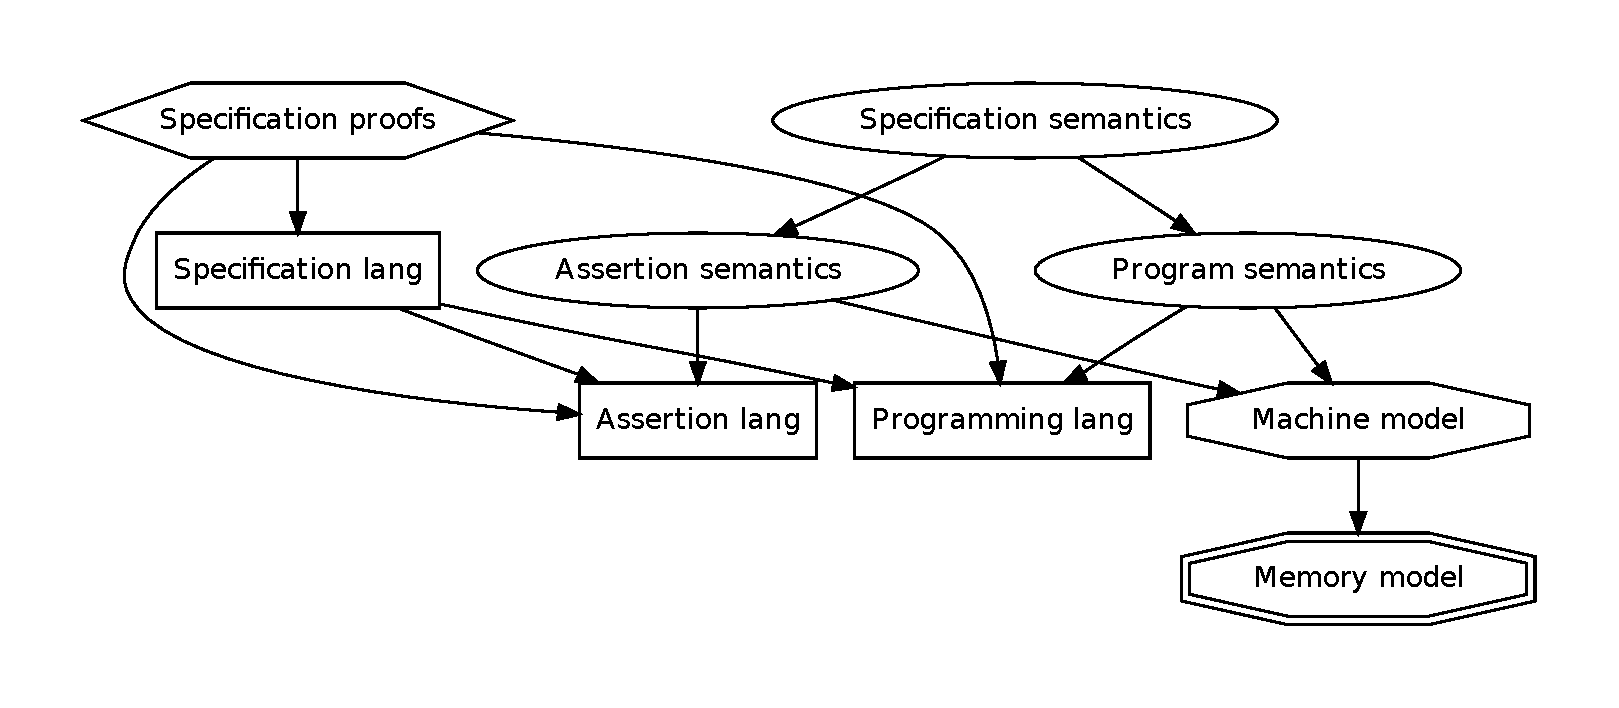
\includegraphics[scale=0.5]{dependency-graph/dg-reduced}
\caption{\label{fig:dependency-graph}Dependency graph for the project.}
\end{center}
\end{figure}

The memory model is shown in a double-lined octagon, which reflects the assumption in this project that it is complete and correct, and is not further modified from its operational definition in \cite{DBLP:conf/tphol/OwensSS09}, which is summarized in Section~\ref{sec:memory-model}. 

The machine model---in particular, the notion of machine state---depends on, but is distinct from, the memory model. For example, the memory model dictates that each processor has a private set of named registers, whereas in the machine models I shall define, a single share set of variable names is assumed. I will also take the liberty in the machine model to relax other restrictions on the notion of state from the memory model, such as the requirement that writes buffered by a single processor are totally ordered. 

The programming language is a structured C-like language with concurrent composition. It does not explicitly depend on any other components of the project. The programming language semantics relates the programming language to the machine model, and hence depends on them both. The machine models, programming language and semantics are described in Section~\ref{sec:programming-language}. 

The assertion language also does not explicitly depend on any other components of the project.\footnote{Implicitly, of course, it depends significantly on the memory and machine models.} The assertion language semantics associates the assertion language to predicates, which are defined later as sets of states (as defined by the machine model) with a particular structure. Assertions and their meaning are described in Section~\ref{sec:assertions}. 

Ideally there would also be a proof theory of assertions and a corresponding soundness theorem. I have chosen not to focus on a proof theory of assertions in this project, but will indicate some semantic implications and equivalences that would be relevant to that end in Section~\ref{sec:algebra}.

The specification language encompasses the programming and assertions languages, and its semantics is given in terms of the semantics of programs and assertions. The proof theory of specifications relies on the existence of a suitable proof theory of assertions for determining entailments. The soundness of the specification logic relies on the the soundness of the proof theory of assertions as well as the semantics of programs and assertions. Specifications are described in Section~\ref{sec:specifications}.

\chapter{Background}

\section{Program Logics}
\label{sec:program-logics}

Given that the motivating problem is to reason about concurrent programs executing on a particular memory model, how might one approach the correctness of the program in Figure~\ref{fig:dekker} and others like it such as concurrent data structures? One solution---perhaps, for now, the best---is to reason directly about the program semantics in the following way:
\begin{enumerate}
\item formalize the semantics of the programming language using a general purpose logic (e.g., first-order logic, higher-order logic, type theory);

\item prove that the semantics agrees with the memory model;

\item characterize the intended program property using the general logic; 

\item prove using the general logic that the semantic object which represents the program at hand possesses this property.
\end{enumerate} 
This is a perfectly reasonable strategy and, by using a proof assistant for a selected general purpose logic (e.g., ACL2 \cite{DBLP:journals/tse/KaufmannM97}, Isabelle/HOL \cite{DBLP:books/sp/NipkowPW02}, or Coq \cite{CoqBook}), is within the realm of feasibility for some programs and some experts. But, due to the generality of the logic and complexity of the semantics of programs under study, one expects such proofs to be exceptionally complex. And although experts would certainly develop methodologies and abstractions to tame this complexity, the desire to reason at a higher and more intuitive level is manifest.

This is just the purpose of a \emph{program logic}, which allows high-level formal reasoning that codifies the programmer's intuition about the behavior and correctness of the program under study. Ideally, the program logic incorporates those methodologies and abstractions that have been most useful to expert users reasoning directly about semantic objects in more general logics.

The situation is analogous to the use of temporal logics for studying reactive systems. Though it is technically possible to reason about about such systems using a general-purpose logic, both human reasoning (e.g., Unity \cite{unity-book}) and automation (e.g., model checking \cite{model-checking}) were facilitated by specialized logics.

\subsection{Hoare Logic}

Hoare introduced the first program logic for an Algol-like language in his seminal 1969 paper \cite{DBLP:journals/cacm/Hoare69}. Programs are specified with a pair of assertions, written in first-order logic, that describe pre- and post-execution system states. The logic has two flavors of specification: partial correctness, $\left\lbrace P \right\rbrace c \left\lbrace Q \right\rbrace$, in which nonterminating executions satisfy any specification; and total correctness, $\left\langle P \right\rangle c \left\langle Q \right\rangle$, in which termination is required to satisfy any specification. 

The axioms and inference rules are mostly directed by the program syntax, making proof construction partially mechanical. Notable exceptions include the inference rule for loops, which requires invention of a suitable loop invariant, and the rule of consequence: \infrule[consequence]{P' \Rightarrow P \,\,\,\,\,\, \left\lbrace P \right\rbrace c \left\lbrace Q\right\rbrace \,\,\,\,\,\, Q \Rightarrow Q' }{\left\lbrace P' \right\rbrace c \left\lbrace Q' \right\rbrace} For correct application of the rule, validity of the first-order logic implications must be proved. But first-order validity is, of course, undecidable in general, so while Hoare logic does ease some of the pain of proof construction, it is not a panacea.

%% Hoare logic has been thoroughly studied since its
%% introduction. Notably, it has been shown to be complete, in the sense
%% that true program specifications are provable if validity of
%% implications between assertions can be determined.

\subsubsection{Separation Logic}

A serious drawback of Hoare logic is its inability to soundly cope with pointer variables, thus severely complicating its application to low-level systems programs. After more than forty years of research, a major breakthrough finally came with Reynolds' invention of \emph{separation logic} \cite{DBLP:conf/lics/Reynolds02}. A Hoare-style program logic (insofar as the axioms and inference rules are similar), the crucial difference between it and Hoare logic is the assertion language. Instead of the first-order logic assertions used by Hoare logic specifications, separation logic makes use of a new logic\footnote{More precisely, a theory of the logic of bunched implications pioneered by O'Hearn, Pym and others \cite{DBLP:journals/bsl/OHearnP99,DBLP:journals/tcs/PymOY04}.}  for describing system states with a notion of a heap, into which pointers point, and disjointness of said states. The salient formulas that capture these notions are the \emph{points-to assertion}, $x \mapsto y$, and the \emph{separating conjunction}, $P * Q$. Models of the first formula are heaps with exactly one address allocated, given by the value of $x$, and with the value of $y$ stored at that address. Models of the second formula are heaps that can be partitioned by address into two subheaps, one of which models the formula $P$ and the other $Q$.

Besides soundness w.r.t.~a sequential C-like language with pointers and dynamic memory management, separation logic is important because it embodies the principle of \emph{local reasoning}. Unlike with Hoare logic, reasoning may be restricted to a program component's \emph{footprint}---i.e., just the part of the system state referenced by the program during its execution---from which one may generalize to complete system states. O'Hearn, Reynolds and Yang informally describe local reasoning in the context of sequential pointer programs as follows \cite{DBLP:conf/csl/OHearnRY01}: \begin{quotation}\noindent To understand how a program works, it should be possible for reasoning and specification to be confined to the [memory addresses] that the program actually accesses. The value of any other [addresses] will automatically remain unchanged.\end{quotation}

Separation logic embodies the principle of local reasoning with its \emph{small axioms} and its \emph{frame rule}. The small axioms describe the programming language's primitive commands, specifying only their respective footprints. For example, the small axiom\footnote{Actually, an axiom schema parametrized by the expressions $e$ and $e'$.} for the store command requires with its precondition only that the relevant location be allocated with some value,\footnote{$e \mapsto -$ is shorthand for $\exists v\,.\,e \mapsto v$.} and the resulting postcondition describes only the result of updating this location: \infax[store]{\left\lbrace e \mapsto -\right\rbrace \,\left[e\right] := e' \,\left\lbrace e \mapsto e'\right\rbrace} The local specification can then be generalized to a global specification using the \emph{frame rule}:\footnote{Some formulations of the frame rule additionally require the syntactic side condition that none of the variables modified by the command $c$ occur freely in $R$.}  \infrule[frame]{\left\lbrace P \right\rbrace c \left\lbrace Q \right\rbrace}{\left\lbrace P*R \right\rbrace c \left\lbrace Q*R \right\rbrace} No similar conjunctive frame rule is sound in Hoare logic, limiting its ability to scale to large programs.

Besides having been used to give human-readable proofs to a variety of algorithms that manipulate complex pointer-based data structures (e.g., the Schorr-Waite graph-marking algorithm \cite{Yang-thesis}), useful fragments of separation logic have been automated as part of program verifiers and static analysis implementations, which have been successfully applied to multi-thousand line programs~\cite{DBLP:conf/fmco/BerdineCO05,DBLP:conf/cav/YangLBCCDO08}.

\subsubsection{Concurrent Logics}

Research into logics for concurrent programs has progressed independently. Early attempts culminated in an extension of Hoare logic by Owicki and Gries \cite{DBLP:journals/cacm/OwickiG76}, which adds a rule for parallel composition of two program components with the cumbersome side condition that every assertion in one component's specification be invariant under the operation of each atomic command executed by the other component. While elegant in its simplicity, the side condition restricts the logic's usefulness. First, every application of the parallel composition rule requires a number of invariant proofs quadratic in the size of the components, making scalability difficult. Second, the side condition creates dependencies on the \emph{proofs} of the component specifications, not just on the specifications themselves. This effectively rules out independent proof construction for the individual components and yields a highly non-compositional logic.

Some relief from these problems was provided by Jones in his rely/guarantee logic \cite{JonesRelyGuar}, in which Hoare-style specifications are augmented with two additional assertions: the \emph{rely} condition, which bounds the interference from the environment that a component can tolerate while still meeting its pre- and post-specifications; and the \emph{guarantee} condition, which bounds the interference the program itself may inflict upon the environment. Application of the rely/guarantee parallel composition rule requires proofs that each process' rely condition subsumes the others' guarantee conditions.

While a considerable improvement over the Owicki-Gries logic---subsumption proofs linear in the number of components versus quadratic in their size, and dependence only among components'specifications instead of their proofs---rely/guarantee still has shortcomings. The logic cannot be considered truly compositional because each component may be specified with a variety of interference conditions, and it is not clear which are appropriate until attempting the parallel composition. Furthermore, it can be laborious to specify sufficiently strong guarantee conditions. For example, the guarantee condition for a component with three variables ($x,y,z$) that updates only one ($x := x+1$) must describe not just the relevant variable change ($x' = x + 1$), but also that all others remain the same ($\ldots \wedge y' = y \wedge z' = z$)---the latter condition being difficult because it suggests a sort of quantification over variable names not possible in first-order logic, instead requiring an explicit numeration of state variables.

\subsubsection{A Marriage of Techniques}

A partial solution to this problem of specification has recently appeared via separation logic. A new concurrent program logic from Vafeiadis and Parkinson, dubbed RG-Sep \cite{DBLP:conf/concur/VafeiadisP07} (``a marriage of rely/guarantee and separation logic''), mates a generalization of separation logic's assertion language and frame rules with the rely/guarantee logic. Besides inheriting the local reasoning features of separation logic, RG-Sep eases the pain of specifying environmental interference by semantically partitioning the system state into private and shared parts. A new class of boxed assertions $\boxed{P}$ is used to describe shared state, and the logical operations are adjusted so that, e.g., a separated conjunction of boxed assertions $\boxed{P} * \boxed{Q}$ allows their footprints to overlap.\footnote{An interesting consequence is that $\boxed{P} * \boxed{Q}$ is logically equivalent to $\boxed{P \wedge Q}$.} The proof rules are then modified so that, e.g., parallel composition requires only that each component be tolerant of environmental interference to shared state, not private state. This could be used in the previous example to obviate the explicit enumeration needed to describe invariance of the irrelevant state variables.

RG-Sep embodies the most advanced ideas about high-level reasoning techniques for fine-grained concurrent shared-memory programs, including local reasoning. Vafeiadis' 2008 dissertation \cite{VafeiadisDissertation} includes correctness proofs for a variety of complex, racey concurrent data structures using the logic. RG-Sep is by no means simple, but does yield relatively concise, readable proofs about difficult algorithms. Indeed, the only significant criticism I provide here is that, as with all the other concurrent logics discussed, RG-Sep is not sound w.r.t.~weak memory models for racey programs.

\section{Memory Consistency Models}

TODO 

\paragraph{Sequential Consistency} 

\subsection{The x86-TSO Memory Model}
\label{sec:memory-model}

This section contains a brief, informal review of the x86-TSO memory model as defined by Owens, Sarkar and Sewell \cite{DBLP:conf/tphol/OwensSS09}. The model is given as a collection of legal traces of memory events. Legal traces are defined axiomatically and operationally, the latter via a labeled transition relation between machine states. These states are four-tuples $(R,m,B,l)$ in which: \begin{itemize}
	\item $R : \setprocessors \tfun \setidentifiers \pfun \setvalues$ is a register file for each processor;
	\item $m : \setlocations \pfun \setvalues$ is a shared memory; 
	\item $B : \setprocessors \tfun \listof{(\setlocations \times \setvalues)}$ is a write buffer for each processor; 
	\item $l : \setprocessors^\bot$ is a global lock. 
\end{itemize}

Transitions (labeled by memory events) between states indicate the possibility and effect of those memory events. For example, in any state $(R,m,B,l)$, processor $p$ may write a value $v$ into its register $i$; i.e., it may update the state such that $R_p(i) = v$. Similarly, if $R_p(i) = v$ then $p$ may read value $v$ from its register $i$. A summary of the other events processor $p$ may perform is as follows: \begin{itemize}
	\item it may load from its write buffer the most recent value of a location---or, if a write to that location is not found in its write buffer, from memory---if the lock is either available ($i.e.$, the lock value is $\bot$) or is held by $p$, but not if some other processor $q \neq p$ holds the lock;
	\item it may store a value to a memory location by adding a new write to the head of its write buffer regardless of the status of the lock; 
	\item it may flush (or, synonymously in this document, commit) the least recent write in its buffer to memory if it holds the lock or the lock is available;  
	\item it may fence if its buffer is empty;
	\item it may acquire the lock (i.e., change the lock value in the current state to $p$) if the lock is available; 
	\item it may release the lock (i.e., change the lock value in the current state to $\bot$) if it holds the lock.
\end{itemize}

This specification bounds the sort of memory events that can occur in program executions, but it does not give meaning to the programs of a particular language. The semantics of the programming language used in this project is however guided by the memory model, and it ought be possible to prove that it respects the bounds of the model. But this is not the focus of this project; and, even without such a correspondence proof, it will still be clear that the semantics of the programming language is manifestly weak. 

\chapter{Basics}
\label{ch:basics}

\section{Mathematical Preliminaries and Notation}

For a set $S$ and object $o \notin S$ we write $S^o \eqdef S \uplus \set{o}$. For example, a domain $S$ can be lifted to its optional domain by writing $S^\bot$. 

\subsection{Relations}
\label{sec:relations}

For any set $A$, we write $\ident{A}$ for the identity relation on $A$. For a binary relation $R$ on $A$ and $n \in \setnaturals$, we write $\relexp{R}{n}$ for the $n$-fold iteration of $A$, defined by induction on $n$ as follows: \begin{align*} \relexp{R}{0} \eqdef &\ident{A} \\ 
\relexp{R}{n+1} \eqdef & \relexp{R}{n} \rcomp R.\end{align*} We write $R$ we write $\tcl{R}$ for the transitive closure of $R$, and $\rtcl{R}$ for its reflexive-transitive closure: \begin{align*}
    \tcl{R} \eqdef \bigcup_{n \in \setpositives} \relexp{R}{n} \text{~~~and~~~}
    \rtcl{R} \eqdef \bigcup_{n \in \setnaturals} \relexp{R}{n} 
\end{align*}

\subsection{Functions}
\label{sec:functions}

For a (possibly partial) function $f : A \pfun B$ and $a \in A$ and $b \in B$, we write $\funup{f}{\ptup{a}{b}}$ for the updated function: \[ \funup{f}{\ptup{a}{b}} \eqdef \lambda x . \begin{cases}
	b & \text{if $x = a$} \\
	f(x) & \text{otherwise.}
\end{cases}\] 

We write $f(a) = \bot$ if the partial function $f$ is not defined at point $a$,i.e. if $a \notin \dom{f}$, and $\defined{f(a)}$ otherwise. The everywhere-undefined function is indicated by $\nil$. The partial sum $f \uplus g$ of partial functions $f$ and $g$ is defined, when $\dom{f} \cap \dom{g} = \nil$, as follows: \[ f \uplus g \eqdef \lambda x . \begin{cases}
    f(x) & \text{if $x \in \dom{f}$} \\
    g(x) & \text{else if $x \in \dom{g}$} \\
    \bot & \text{otherwise.}
\end{cases}\]

 When convenient, we also write $f_a$ as shorthand for $f(a)$. $a \mapsto b$ is shorthand for the unique partial function $f$ such that $f(a) = b$ and is undefined otherwise. For $A' \subseteq A$, $\restrict{f}{A'}$ is the restriction of $f$ to domain $A'$. 

For (possibly partial) functions $f,g : A \pfun B$, we we write $f \override g$ for the result of \emph{overriding} $f$ with $g$: \[ f \override g \eqdef \lambda x . \begin{cases}
	g(x) & \text{if $x \in \dom{g}$} \\
	f(x) & \text{otherwise.}
\end{cases} \] An obvious property is that, if $g(a) = b$, for some $b \in B$, then also $(f \override g)(a) = b$. Some additional properties follow in Lemma~\ref{lem:override}. 

\begin{lemma}
    \label{lem:override}
    Let $f,g,h : A \pfun B$. 
    \begin{enumerate}
        \item $f \override \nil = \nil \override f = f$
        \item $f \override (g \override h) = (f \override g) \override h$. 
        \item $\dom{f \override g} = \dom{f} \cup \dom{g}$. 
        \item If $\dom{f} \cap \dom{g} = \nil$ then $f \override g = f \uplus g$, and hence $f \override g = g \override f$. 
    \end{enumerate}
\end{lemma}

\subsection{Lists}
\label{sec:lists}

The empty list is denoted by $\lnil$, the literal list by $\llit{o,\ldots, o'}$, list construction by $o \lcons l$, and list concatenation by $l \lapp l'$, for objects $o$ and lists $l$. We write $\listof{\mathcal{T}}$ to indicate lists of elements drawn from the set $\mathcal{T}$. 

For a list $l : \listof{(A \times B)}$, we write $\funof{l}$ for the corresponding partial lookup function: \[ \funof{l} \eqdef \lambda x .\begin{cases}
	b &\text{ if $l = l' \lapp \llit{(x,b)}$}\\
	\funof{l'}(x) &\text{ if $l = l' \lapp \llit{(y,b)}$ with $x \neq y$}\\
	\bot & \text{otherwise.}
\end{cases}\] For $A' \subseteq A$, $\restrict{l}{A'}$ is the sublist restriction of $l$ to domain $A'$.

For convenience, we lift these function definitions pointwise to sets of lists. E.g., for a set $L$ of lists, $a \lcons L \eqdef \setof{a \lcons l}{l \in L}$. 

The set of \emph{interleavings} of lists $m,n$, written $m \merge n$, is defined by recursion on the structure of $m$ and $n$: \begin{align*}
	m \merge \lnil & = \lnil \merge m = \set{m} \\ 
	a \lcons m' \merge b \lcons n' & = a \lcons (m' \merge (b\lcons n')) \uplus b \lcons ((a \lcons m') \merge n').
\end{align*}

We now define a subset of the interleavings of lists of pairs from $A \times B$ that play an analogous role to to function overriding. The result of overriding a list $m$ with another $n$, written $m \override n$, is defined as follows: \[ l \in m \override n \iffdef \funof{l} = \funof{m} \override \funof{n}.\] As with function overriding, list overriding has the property that, if $\funof{n}(a) = b$, for some $b \in B$, and $l \in m \override n$, then $\funof{l}(a) = b$. Because all elements of $m \override n$ have the same lookup function, we may safely extend the list lookup notation as follows: \[ \funof{m \override n} \eqdef \lambda x . \funof{l}(x),\] for arbitrary $l \in m \override n$. 

As for function overriding, list overriding has the basic property that, if $a \in \dom{\funof{n}}$, then $\funof{n}(a) = \funof{n \override m}(a)$. It also has the other following analogous properties, as noted by Lemma~\ref{lem:list-override}. 
\begin{lemma}
    \label{lem:list-override}
    Let $l,m,n : \listof{A \times B}$. 
    \begin{enumerate}
        \item $l \override \nil = \nil \override l = l$
        \item $l \override (m \override n) = (l \override m) \override n$. 
        \item $\dom{\funof{m \override n}} = \dom{\funof{m}} \cup \dom{\funof{n}}$. 
        \item If $\dom{\funof{m}} \cap \dom{\funof{n}} = \nil$ then $m \override n = m \merge n$, and hence $m \override n = n \override m$. 
    \end{enumerate}
\end{lemma}

\section{Universes}

The various universal sets are declared and in some cases defined in Figure~\ref{fig:universes}. Note that, in the case of memory locations (i.e., addresses) and processor identifiers, 0 is excluded. 

\begin{figure}[ht]
	\centering
	\begin{tabular}{rcl|l}
		\multicolumn{3}{c}{Set} & Description \\ \hline
		\multicolumn{3}{l|}{$\setidentifiers$} & Identifiers \\
		$\setvalues$ & $=$ &  $\setintegers$ & Values \\
		$\setlocations$ & $\subseteq$  &  $\setpositives$ & Memory locations \\
		$\setprocessors$ &$\subseteq$ &  $\setpositives$ & Processor identifiers
	\end{tabular}
	\caption{\label{fig:universes}Universal Sets}
\end{figure}

\section{Expressions and Stacks}
\label{sec:expressions}

Expressions are terms that denote values, which in this development are just integers. Hence, they are also used later on to denote memory locations and processor identifiers. 

The language of expressions, written $\exprs$, is given by the following grammar: \[ \exprs~e \bnfdef v \bnfbar x \bnfbar (e + e') \bnfbar (e - e') \bnfbar \ldots, \] where $v \in \setvalues$ and $x \in \setidentifiers$. (The possibility of additional operations is left open; the complete set of expression is not important.)

The semantics of expressions is given w.r.t.~\emph{stacks}, which are total functions from $\setidentifiers$ to $\setvalues$. The collection of functions $\setidentifiers \tfun \setvalues$ is abbreviated $\setstacks$. The interpretation of an expression w.r.t.~a stack $s$ is given by the \emph{extension} of a stack, written $\ext{s}$, which is a total function from $\exprs$ to $\setvalues$ defined as follows: \begin{align*}
    \ext{s}(v) \eqdef & v \\
    \ext{s}(x) \eqdef & s(x) \\
    \ext{s}(e + e') \eqdef & \ext{s}(e) + \ext{s}(e') \\
    \ext{s}(e - e') \eqdef & \ext{s}(e) - \ext{s}(e')
\end{align*}  

Boolean expressions are terms that denote truth values. Their language is given by the following grammar: \[ \bexprs~b \bnfdef \bexpf \bnfbar \bexpt \bnfbar (!b) \bnfbar (e = e') \bnfbar \ldots, \] where $e,e' \in \exprs$. For convenience, we represent truth values by the set $\set{0,1}$ so the extension of a stack can also be used to interpret boolean expressions: \begin{align*}
    \ext{s}(\bexpf) \eqdef & 0 \\
    \ext{s}(\bexpt) \eqdef & 1 \\
    \ext{s}(!b) \eqdef & 1 - \ext{s}(b) \\
    \ext{s}(e = e') \eqdef & \begin{cases}
        1 &\text{ if } \ext{s}(e) = \ext{s}(e')\\
        0 &\text{ otherwise.}
    \end{cases}
\end{align*}

The set of \emph{free variables} of a (boolean) expression $e$, written $\fv{e}$, is defined as usual: \begin{align*}
    \fv{v} \eqdef & \nil \\ 
    \fv{x} \eqdef & \set{x} \\ 
    \fv{e + e'} \eqdef & \fv{e} \cup \fv{e'} \\ 
    \fv{e - e'} \eqdef & \fv{e} \cup \fv{e'} \\ 
    \fv{\bexpf} \eqdef & \nil \\ 
    \fv{\bexpt} \eqdef & \nil \\ 
    \fv{!b} \eqdef & \fv{b} \\ 
    \fv{e = e'} \eqdef & \fv{e} \cup \fv{e'}
\end{align*}

For stacks $s,s'$ and $X \subseteq \setidentifiers$, we write $s \stcong{X} s'$ if, for all $x \in X$, $s(x) = s'(x)$. The following basic lemma uses this relation to connect the static and dynamic semantics of expressions. 
\begin{lemma}
\label{lem:exp-stcong}
    If $s \stcong{\fv{e}} s'$ then $\ext{s}(e) = \ext{s'}(e)$. 
\end{lemma}

\begin{proof}
By induction on the structure of the expression $e$. 
\end{proof}

\chapter{A Sequential Program Logic}
\label{ch:uniprocessor}

In this chapter we describe a program logic for a sequential, single-processor, weak-memory programming model. The semantics of programs and assertions will be given in terms of system states with a single write buffer, and the logic is tailored to reason about the behavior of sequential programs w.r.t.\ these states. The logic developed in this chapter is not especially useful; the behavior of sequential program execution on this model is essentially the same as on the typical, strong-memory model (in which memory is modeled as a single array of addresses), and existing logics for reasoning this behavior are certainly simpler than the one developed here. But the sequential program logic is a pedagogical stepping stone toward the current program logic, for which the behavior of programs may well be significantly different from that of a strong-memory model. The development of the sequential logic is vastly simpler than weak-memory multi-processor logic, and many of the more difficult issues in that task can be introduced and explained more easily in a single-processor setting. 

A detailed description and soundness proof of a single-processor, weak-memory program logic was given previously in \cite{wmsldetails}. 

\section{A Sequential Example}

Consider the following simple sequential program $c$, which stores the value 1 at an address $x$, flushes that value back to memory with a fence instruction, and then loads the value in memory from address $x$ into variable $y$: \[ c \eqdef \cseq{\cstore{x}{1}}{\cseq{\cfence}{\cload{y}{x}}}.\] This sequential program will fail with a memory error if the value of $x$ is not properly allocated memory address; any provable specification of this program must require that this holds of $x$ initially. If the value of $x$ is indeed an allocated address, then upon termination the write buffer will be empty and the value in memory at location $x$ will be equal to $y$, which is itself equal to 1. 

In the program logic developed in this chapter, we express this informal specification of $c$ with the following formal specification: \begin{align}\label{eq:seq-ex-spec} \triple{x \fpointsto -}{c}{x \fpointsto y}.\end{align}
We write $x \fpointsto y$ in the postcondition to indicate that the value of $x$ is an allocated memory address, and that the value of memory at that address is equal to the value of $y$. In the precondition, the particular value of memory at $x$ is unimportant, so write $x \fpointsto -$.  

A \emph{proof sketch} of the program specification in Equation~\ref{eq:seq-ex-spec} is as follows:
\Calc{
  
  \conn{}{$x \fpointsto -$}

  $\cstore{x}{1}$

  \conn{}{$x \fpointsto - \fseq x \fwriteu 1$}

  $\cfence$

  \conn{}{$x \fpointsto 1$}

  $\cload{y}{x}$

  \conn{}{$x \fpointsto y$}

}
As the name indicates, a proof sketch provides a skeleton of a complete proof of a program specification. For a program $c_1 \opseq c_2$, a proof sketch: \Calc{

  \conn{}{$P$}

  $c_1$

  \conn{}{$R$}

  $c_2$

  \conn{}{$Q$}

} indicates that a complete proof will include proofs of the sub-specifications $\triple{P}{c_1}{R}$ and $\triple{R}{c_2}{Q}$, which will be combined in the last step using a rule of inference (\textsc{seq}) for composing specifications of sequentially combined commands: 
\[ \infer[{\textsc{seq}}]{\triple{P}{c_1 \opseq c_2}{Q}}{\infer{\triple{P}{c_1}{R}}{\vdots} & \infer{\triple{R}{c_2}{Q}}{\vdots}}\] where the vertical dots represent the remaining proofs to be supplied. 

Returning to the proof sketch of the program specification in Equation~\ref{eq:seq-ex-spec}, we see that to complete the proof we must derive three sub-specifications, one for each primitive command: \begin{enumerate}
  \item $\triple{x \fpointsto -}{\cstore{x}{1}}{x \fpointsto - \fseq x \fwriteu 1}$
  \item $\triple{x \fpointsto - \fseq x \fwriteu 1}{\cfence}{x \fpointsto 1}$
  \item $\triple{x \fpointsto 1}{\cload{y}{x}}{x \fpointsto y}$
\end{enumerate}
The first specification asserts that the result of storing the value 1 to the valid address $x$ results in the addition of a buffered write, which may later commit to memory and overwrite the current value, which remains unspecified. The second specification asserts that the result of explicitly flushing the write to memory with a fence command overwrites the existing value with the new value $1$. The third specification asserts that, as a result of loading the value in memory at address $x$ into variable $y$, the value in memory at address $x$ becomes equal to $y$. 

We shall now derive these three specifications. For the first specification, note that store command $\cstore{x}{1}$ \emph{buffers} a new write, which may be flushed to memory later. We write $x \fwriteu 1$ to indicate a buffered write to memory address $x$ with value 1, and $x \fpointsto - \fseq x \fwriteu 1$ to describe the \emph{temporal composition} of the shared memory value $x \fpointsto -$ and the buffered write $x \fwriteu 1$, where the left-hand side precedes the right-hand side. The first specification can be derived directly from the axiom for the store command: 
\[ 
\infer[\textsc{store}]{\triple{x \fpointsto -}{\cstore{x}{1}}{x \fpointsto - \fseq x \fwriteu 1}}{}
\]

For the second specification, note that fence command flushes all buffered writes to main memory. In this case, the result of flushing the buffered write $x \fpointsto - \fseq x \fwriteu 1$ yields $x \fpointsto 1$. The axiom for the fence command allows us to additively conjoin to any precondition $P$ an assertion $\fbaru$ that ensures all writes have indeed flushed. Hence, we may derive $(x \fpointsto - \fseq x \fwriteu 1) \conj \fbaru$. This assertion, although not equal to the desired postcondition of $x \fpointsto 1$, is logically equivalent, and so we may use the \emph{rule of consequence} to derive the second specification as follows:
\[ 
  \infer[\textsc{cons}]{\triple{x \fpointsto - \fseq x \fwriteu 1}{\cfence}{x \fpointsto 1}}{\infer[\textsc{fence}]{\triple{x \fpointsto - \fseq x \fwriteu 1}{\cfence}{(x \fpointsto - \fseq x \fwriteu 1) \conj \fbaru}}{}}
\]

For the third specification, we can use an instance of the \textsc{load-mem} axiom scheme to show that the result of evaluating the store command $\cstore{y}{x}$ from precondition $x \fpointsto 1$ yields the postcondition $x \fpointsto 1 \conj y = 1$. Once again, this is not equal to the desired postcondition of $x \fpointsto y$, but it is logically equivalent. Hence, we derive the third specification using the axiom and the rule of consequence: 
\[ 
  \infer[\textsc{cons}]{\triple{x \fpointsto 1}{\cload{y}{x}}{x \fpointsto y}}{\infer[\textsc{load-mem}]{\triple{x \fpointsto 1}{\cload{y}{x}}{x \fpointsto 1 \conj y = 1}}{}}
\]
This completes the proof of the program specification of Equation~\ref{eq:seq-ex-spec}. In the following sections, the notions of program, assertion, specification, and proof are formally defined and discussed. 


\section{Sequential Programs}
\label{sec:sequential-programs}

In this chapter, programs are identified with \emph{sequential commands}, which consist of compositions of \emph{primitive commands} for testing, accessing and modifying state. 

The syntax of primitive commands is given by the following grammar: \begin{align*} \pcomms~p \bnfdef & \cskip \bnfbar \cassume{b} \bnfbar \cassert{b} \bnfbar \cassign{x}{e} \bnfbar \cload{x}{e} \bnfbar \\ 
    & \cstore{e}{e'} \bnfbar \cfence
\end{align*}

The informal meaning of the primitive commands is as follows. \begin{itemize}
    \item $\cskip$ takes no evaluations steps;
    \item $\cassume{b}$ evaluates to $\cskip$ if $b$ holds and becomes stuck otherwise; 
    \item $\cassert{b}$ evaluates to $\cskip$ if $b$ holds and aborts otherwise;
    \item $\cassign{x}{e}$ assigns $e$ to identifier $x$; 
    \item $\cload{x}{e}$ assigns the value at memory address $e$ to identifier $x$; 
    \item $\cstore{e}{e'}$ stores the value $e'$ to memory address $e'$; and
    \item $\cfence$ commits any buffered writes to memory 
\end{itemize}

The formal semantics of the successful execution of a primitive command $p$ is given as a transition relation between machine states $\sigma,\sigma'$ \[ p : \sigma \step \sigma'. \] Informally, a triple $p,\sigma,\sigma'$ belongs to this relation if the successful execution of $p$ in state $\sigma$ may yield state $\sigma'$. (A formal interpretation will be given later in the context of a formal semantics of full commands.) A primitive command may alternatively execute unsuccessfully, indicated as follows \[ p : \sigma \step \abort. \] Executions may be unsuccessful as a result of failed assertions---e.g., $\cassert{\bexpf}$ is unsuccessful from any state---or attempts to access or modify a memory location outside a command's address space. We say that a primitive command $\emph{aborts}$ in such unsuccessful executions. 

To define these relations formally, we must first define the notion of a uniprocessor memory system and a machine state. 

\begin{definition}
A \emph{uniprocessor memory system} is a pair $(h,B)$, where: \begin{itemize}
    \item $h : \setlocations \pfun \setvalues$ is a \emph{heap}, i.e., a partial function that represents the allocated locations of shared memory and their values; and 
    \item $B : \listof{(\setlocations \times \setvalues)}$ is a write buffer;
\end{itemize}
\end{definition} 
The set of uniprocessor memory systems is abbreviated as $\setmemorysystems$.
The pair that consists of a stack $s$, as defined in Section~\ref{sec:expressions}, which assigns values to identifiers, and a memory system $\mu$ is called a \emph{state}, typically abbreviated by $\sigma$. The collection of states is written $\setstates$. We often abuse notation by interchanging memory systems and states in definitions for which the stack is irrelevant. 

Note that the notion of machine state given here differs from that used to define the memory model. First and most obviously, there is only a single write buffer, because in this section we are discussing only the exection of sequential programs on uniprocessor machines. Second, the global lock value from the memory model is omitted because there is only one write buffer, and hence commands have no need to claim sole ownership of the memory system. Third, the set of names (i.e., ``registers,'' ``variables,'' ``identifiers,'' etc.) are global instead of local to each processor. This is for convenience only, and is not a technical restriction. The specification logic will be restricted to programs for which the names are partitioned among processes, except for those that are never modified to. Another reasonable choice would have been to use local names only, and to share read-only values among processes in the shared memory. This has the advantage of codifying the the above healthiness condition on programs directly into the model of the language and logic; it has the disadvantage of (perhaps) describing access to shared values slightly more awkward. 

The definition of the semantic relation for primitive commands is given in Figure~\ref{fig:primitive-semantics}. By \textsc{p-assume}, the primitive $\cassume{b}$ takes an evaluation step only if the boolean expression $b$ evaluates to $1$ in the current state. Otherwise, it is effectively stuck. Later, when we describe the specification logic, we will see that such stuck executions are irrelevant to the truth of specification. In fact, stuck executions are equivalent to diverging executions w.r.t.\ the specification logic. By \textsc{p-assert} and \textsc{p-assert-a}, $\cassert{b}$ either evaluates normally if the boolean expression $b$ evaluates to 1 in the current state, and aborts otherwise. An aborting command will later be shown to not satisfy any specification. By \textsc{p-assign}, the assignment primitive $\cassign{x}{e}$ always evaluates successfully by assigning to $x$ the value of the expression $e$ in the current state. By \textsc{p-load}, the load primitive $\cload{x}{e}$ assigns to $x$ the value of the most recent buffered write to the address that is the value of expression $e$, if such a write exists, and otherwise gives the value in the current heap at at that address. If the address that is the value of expression $e$ has neither any buffered writes nor is defined in the heap (i.e., if $\ext{s}(e) \notin (h \override \funof{b})$) then by \text{p-load-a} the load primitive aborts. By \textsc{p-store}, the store primitive $\cstore{e}{e'}$ appends to the write buffer a new write with address the value of expression $e$ and value the value of $e'$, but only if the value of $e$ is an address that is already allocated (i.e., if $\ext{s}(e) \in \dom{h \override \funof{b}}$). Otherwise, by \textsc{p-store-a} the store primitive aborts. Finally, by \textsc{p-fence}, the $\cfence$ primitives evaluates without changing the state if the write buffer is empty. Later, when we describe the semantics of full commands, we will explain how the fence primitive can be thought to flush a non-empty buffer. 

\begin{figure}[p]
    \centering

    \begin{minipage}{\columnwidth}

        \infrule[p-assume]{\text{ if  $\ext{s}(b) = 1$}}{\cassume{b} : (s,h,b) \step (s,h,b)}

        \vspace{1em}

        \infrule[p-assert]{\text{ if  $\ext{s}(b) = 1$}}{\cassert{b} : (s,h,b) \step (s,h,b)}

        \vspace{1em}

        \infrule[p-assert-a]{\text{ if  $\ext{s}(b) = 0$}}{\cassert{b} :(s,h,b) \step \abort}

        \vspace{1em}

        \infrule[p-assign]{}{\cassign{x}{e} :(s,h,b) \step (\funup{s}{\ptup{x}{\ext{s}(e)}},h,b)}

        \vspace{1em}

        \infrule[p-load]{\text{if $(h \override \funof{b})(\ext{s}(e)) = v$ and $i \notin k$}}{\cload{x}{e} :(s,h,b) \step (\funup{s}{\ptup{x}{v}},h,b)}

        \vspace{1em}


        \infrule[p-load-a]{\text{if $(h \override \funof{b})(\ext{s}(e)) = \bot$ and $i \notin k$}}{\cload{x}{e} :(s,h,b) \step \abort}
        
        \vspace{1em}

        \infrule[p-store]{\text{if $\ext{s}(e) \in \dom{h \override \funof{b}}$}}{\cstore{e}{e'} :(s,h,b) \step (s,h,b \lapp \llit{\ext{s}(e),\ext{s}(e')})}
        
        \vspace{1em}

        \infrule[p-store-a]{\text{if $\ext{s}(e) \notin \dom{h \override \funof{b}}$}}{\cstore{e}{e'} :(s,h,b) \step \abort}
        
        \vspace{1em}

        \infrule[p-fence]{\text{if $b = \lnil$}}{\cfence :(s,h,b) \step (s,h,b)}

    \end{minipage}
    \caption{\label{fig:sequential-primitive-semantics} Semantics of sequential primitive commands}
\end{figure}


Structured commands consist of either a primitive command; a sequential composition of commands; a nondeterministic choice between commands; or an iteration of a command. The language of commands is defined by the following grammar: \[ \comms~c \bnfdef p_e \bnfbar (\cseq{c}{c'}) \bnfbar (\cchoice{c}{c'}) \bnfbar \cloop{c},\] where $p$ is a primitive command.  

The formal semantics of the successful execution of a command is given as a binary transition relation between command-state pairs: \[ c,\sigma \step c',\sigma'.\] But a command's execution may abort unsuccessfully as well, as with primitive commands. Unsuccessful executions are modeled as a transition relation between command-state pairs and an erroneous pseudo-state, as for primitive commands: \[ c,\sigma \step \abort. \] We refer collectively to command-state pairs and the erroneous state $\abort$ as \emph{configurations}, and use $\mathcal{C}$ to indicate a configuration. A configuration $\mathcal{C}$ is considered \emph{safe} if it does not abort: $\mathcal{C} \nostep \abort$.

The semantics of commands also encompasses ``silent'' transitions, which represent the flushing of buffered writes to the shared memory as allowed by the memory model. This flushing is described by a relation $\taustep$ between memory systems\footnote{As noted earlier, we abuse notation by interchanging the concept of state and memory system in definitions for which the stack is irrelevant. Hence, the definition of the relation between memory systems  also constitutes the definition of a relation between states such that $(s,\mu) \taustep (s,\mu')$ iff $\mu \taustep \mu'$.} defined as follows: \begin{align*} (h,b \lapp \llit{(\ell,v)}) \taustep (\funup{h}{\ptup{\ell}{v}},b) 
\end{align*} We write $\taurefines$ as shorthand for the reflexive-transitive closure $\taustep$. 

The complete relation that defines the semantics of commands is given in Figure~\ref{fig:sequential-command-semantics} below. The semantics of primitive commands is lifted directly to the level of commands by \textsc{c-prim} and \textsc{c-prim-a}. The silent transitions as defined by the $\taustep$ relation are also lifted directly to the level of commands by \textsc{c-tau}. Sequential compositions $\cseq{c_1}{c_2}$ evaluate from left-to-right: by \textsc{c-seq} and \textsc{c-seq-a} if the left command $c_1$ evaluates or aborts, then so does the sequential composition; and by \textsc{c-seq-s}, once the left command $c_1$ has evaluated fully to $\cskip$ it is dropped so that evaluation of the right side $c_2$ may proceed. By \textsc{c-ch-1} and \textsc{c-ch-2}, a the nondeterministic choice command $\cchoice{c_1}{c_2}$ may evaluate to either $c_1$ or $c_2$, afterward continuing evaluation of the chosen command. Finally, by \textsc{c-loop}, a looping command $\cloop{c}$ may always evaluate without modifying the state by expanding to a nondeterministic choice between doing nothing (i.e., exiting the loop) and sequential composition that consists of evaluating the loop body $c$ once and then continuing with the loop. 

The reflexive-transitive closure of command evaluation relation, written $c,\sigma \rtstep \mathcal{C}$, is defined as usual. The \emph{range} of a configuration $\mathcal{C}$, written \range{\mathcal{C}}, is defined as the set of states $\sigma$ for which $\mathcal{C} \rtstep \cskip,\sigma$. 

\begin{figure}[ht]
    \centering

    \vspace{1em}

    \infrule[c-prim]{\text{ if $p : \sigma \step \sigma'$ and $\sigma' \in \setstates$}}{p,\sigma \step \cskip,\sigma'}

    \vspace{1em}

    \infrule[c-prim-a]{\text{ if $p : \sigma \step \abort$}}{p,\sigma \step \abort}

    \vspace{1em}

    \infrule[c-tau]{\text{if $\sigma \taustep \sigma'$}}{c,\sigma \step c,\sigma'}

    \vspace{1em}

    \infrule[c-seq]{c,\sigma \step c_0,\sigma'}{(\cseq{c}{c'}),\sigma \step (\cseq{c_0}{c'}),\sigma'}

    \vspace{1em}

    \infrule[c-seq-a]{c,\sigma \step \abort}{(\cseq{c}{c'}),\sigma \step \abort}

    \vspace{1em}

    \infrule[c-seq-s]{}{(\cseq{\cskip}{c'}),\sigma \step c',\sigma}

    \vspace{1em}

    \infrule[c-ch-1]{}{(\cchoice{c}{c'}),\sigma \step c,\sigma}

    \vspace{1em}

    \infrule[c-ch-2]{}{(\cchoice{c}{c'}),\sigma \step c',\sigma}

    \vspace{1em}

    \infrule[c-loop]{}{\cloop{c},\sigma \step (\cchoice{\cskip}{(\cseq{c}{\cloop{c}})}),\sigma}

    \caption{\label{fig:sequential-command-semantics} Semantics of sequential commands}
\end{figure} 
 
\paragraph{Sequential Command Abbreviations} A few standard command abbreviations are shown in Figure~\ref{fig:sequential-command-abbreviations}. Some would benefit greatly from local variable declarations, which I have not yet added to the language. 

\begin{figure}[ht]
    \centering
    \resizebox{\columnwidth}{!}{
    \begin{minipage}{\columnwidth}
    \begin{align*}
        \cifthenelse{b}{c}{c'} \eqdef & \cchoice{(\cseq{\cassume{b}}{c})}{(\cseq{\cassume{!b}}{c'})} \\
        \cifthen{b}{c} \eqdef & \cchoice{(\cseq{\cassume{b}}{c})}{(\cseq{\cassume{!b}}{\cskip})} \\
        \cwhile{b}{c} \eqdef & \cseq{\cloop{(\cseq{\cassume{b}}{c})}}{\cassume{!b}}
    \end{align*}
\end{minipage}}
    \caption{\label{fig:sequential-command-abbreviations} Command abbreviations}
\end{figure}

\paragraph{Static Semantics} The static semantics of expressions, primitive commands and commands, embodied here by functions $\fv{-}$ and $\mod{-}$ associating these objects to their sets of free and modified variables, respectively, are completely standard. (Especially so because there is are no name-hiding operations in the language, like the aforementioned missing local variable declaration command.) E.g., $\fv{\cload{x}{y+1}} = \set{x,y}$ and $\mod{\cload{x}{y+1}} = \set{x}$.  

\section{Locality and Separation}
\label{sec:locality}

This section gives an informal introduction to the the notion of local reasoning, including a rough sketch of the idea of a local command. The latter will be codified formally later in the semantics of program specifications in Section~\ref{sec:sequential-specifications}. 

The idea of local reasoning is as follows. Perhaps we wish to show that result of evaluating a command $c$ in a particular state $\sigma$ is always included in a predicate $S$---i.e., that the configuration $c,\sigma$ does not abort, and that if $c,\sigma \rtstep \cskip,\sigma'$ then $\sigma' \in S$. Suppose the elements of the predicate $S$ are all composed of elements from some other predicates $S_0$ and $S_1$---i.e., $\sigma \in S$ iff, for some $\sigma_0 \in S_0$ and $\sigma_1 \in S_1$, $\sigma = \sigma_0 \bullet \sigma_1$---and the initial state $\sigma = \sigma_0 \bullet \sigma_1$ with $\sigma_0 \in S_0$. In that case, we may wish to reduce the original problem to the potentially simpler task of showing that the result of evaluating $c$ in state $\sigma_1$ is always included in $S_1$---i.e., showing that the configuration $c,\sigma_1$ does not abort and that if $c,\sigma_1 \rtstep \cskip,\sigma'_1$ then $\sigma'_1 \in S_1$. 

Under what circumstances is this reduction sound? First, it should be the case that if the command does not abort in the local state $\sigma_1$ then neither does it in the global state $\sigma = \sigma_0 \bullet \sigma_1$. Or, contrapositively, if $c,(\sigma_0 \bullet \sigma_1) \step \abort$ then $c,\sigma_1 \step \abort$. This is called the \emph{safety monotonicity} property. Second, it should be the case that if $c,(\sigma_0 \bullet \sigma_1) \rtstep \cskip,\sigma'$, then there exists $\sigma'_1$ such that $\sigma' = \sigma_0 \bullet \sigma'_1$ and $c,\sigma_1 \rtstep \cskip,\sigma'_1$. For then, by assumption $\sigma_0 \in S_0$, by the reduction $\sigma'_1 \in S_1$, and by the structure of $S$ $\sigma_0 \bullet \sigma'_1 = \sigma' \in S$. This is called the \emph{frame} property. A command that satisfies both the safety monotonicity and frame properties is called a \emph{local command} \cite{DBLP:conf/fossacs/YangO02}. 

For example, $c$ is perhaps a command that reads and writes a particular set of memory addresses, and the starting state $\sigma$ perhaps describes the value of some addresses that are superfluous to the execution of $c$. We may decompose $\sigma$ by partitioning the memory addresses it describes into states $\sigma_0$ and $\sigma_1$ such that $(\sigma_0 \bullet \sigma_1)$, with $\sigma_1$ describing just the memory locations accessed by $c$ and the remainder by $\sigma_0$. Because $(\sigma_0 \bullet \sigma_1)$ contains all the memory addresses of $\sigma_1$ and more, then if $c$ can execute successfully (i.e., without aborting) from state $\sigma_1$ then it can also execute successfully from $\sigma$. And because the addresses of $\sigma_0$ are irrelevant to the evaluation of $c,\sigma$, those addresses will remain unchanged in the resultant state $\sigma'$, and hence $c,\sigma_1$ also evaluates to $\sigma'_1$ with $\sigma' = \sigma_0 \bullet \sigma'_1$. 

This is the essence of local reasoning: leveraging some local property of a command in a local state to a related global property of the command in a global state. Of course, local reasoning is not possible for all properties---it relies crucially on the notion of decomposition $\bullet$---but when it is possible, it offers an especially direct path to showing the desired property. If the commands of a programming language are local, then the principle of local reasoning can be codified into a program logic by way of a \emph{frame rule}, which allows inference from local to global program specifications. This will be considered in more detail in Section~\ref{sec:specifications}. 

In the example above, the state was separated by memory address. But in the programming model described in Section~\ref{sec:sequential-programs}, memory systems consist of both committed and buffered writes. How should we decompose (or separate) a memory system with buffered writes? Or, alternatively, how and when can we compose two partial memory systems? The goal of the next few sections is to carefully define a handful of different, useful notions of separation for which the sequential commands of the programming language are local. Each notions of separation will eventually yield a different frame rule, and hence a different principle of local reasoning about program specifications. 

\subsection{Spatial Separation}
\label{sec:sequential-spatial-separation}

In this section we carefully define a notion of separation for uniprocessor states analogous to the one described in the previous section, in which states are decomposed according by memory address. This is accomplished by defining a notion of separation for memory systems, and then lifting that function to states that have identical stacks: i.e., given a definition of $\mu \bullet \mu'$, the lifted partial function on states $(s,\mu) \bullet (s',\mu')$ is defined as follows \[ (s,\mu) \bullet (s',\mu') \eqdef (s,\mu \bullet \mu') \text{~if $s = s'$ and $\mu \bullet \mu'$ is defined.}\] In the sequel, we shall ignore the distinction between the function on memory systems and the lifted function on states. 

States are typically separated by the resources they describe. In the heaps model of separation logic, the resource is a flat shared memory and the heaps are separated according to address: \[ h_0 \fsep h_1 \eqdef \begin{cases}
    h_0 \uplus h_1 & \text{if $\dom{h_0} \cap \dom{h_1} = \nil$} \\ 
    \bot & \text{otherwise.}
\end{cases}\] Note that the partial function is defined only when the heaps have disjoint domains. It is also, very obviously, commutative. 

We wish to define an analogous notion of separation for memory systems, which consist of a heap-write buffer pairs. As in the case of separation logic, we add heaps with disjoint domains. But how should we combine the write buffers? To ensure commutativity of the operation, a natural choice is to \emph{interleave} writes of the buffers: \[ (h_0,b_0) \fsep (h_1,b_1) \eqdef \bigcup_{b \in b_0 \merge b_1}
    \setof{(h_0 \uplus h_1, b)}{\dom{h_0,b_0} \cap \dom{h_1,b_1} = \nil}
\] Above, we write $\dom{h,b}$ as shorthand for $\dom{h} \cup \dom{b}$. The set $\mu_0 \fsep \mu_1$ is called the \emph{spatial separation} of $\mu_0$ and $\mu_1$ because it requires disjointness of the constituent domains, and does not constrain the order of of the buffered writes. (In a later section, we will weaken the disjointness requirement to yield a weaker notion of separation.)

Interleaving the write buffers results in a notion of separation in which the relative ordering between the writes in the constituent buffers, which necessarily have distinct memory locations, is irrelevant. For example, for $\mu_0 = (\nil,\llit{(\ell,v)})$ and $\mu_1 = (\nil,\llit{(m,u)})$, with $\ell \neq m$, we have both $(\nil,\llit{(\ell,v),(m,u)}) \in (\mu_0 \fsep \mu_1)$ and $(\nil,\llit{(m,u),(\ell,v)}) \in (\mu_0 \fsep \mu_1)$. 

Unlike for the heap separation function, the heap-buffer separation function maps into the power-domain of memory systems: for compatible pairs of memory systems, the separation yields a memory system for each possible interleaving of the individual write buffers. The resulting set is non-empty if and only if the domains of the constituent memory systems are disjoint.\footnote{This is more convenient than defining a partial function into the power-domain. In that case, both $\bot$ and $\nil$ would apparently both indicate incompatibility.} This necessitates a slight change to the definition of a local command, as explained in Section~\ref{sec:locality}. Given a notion of separation that yields a set of memory systems, the safety monotonicity and frame properties must hold for each possible result: i.e., for every $\mu \in \mu_0 \fsep \mu_1$, if $c,\mu$ is safe then so is $c,\mu_1$; and if $c,\mu \rtstep \cskip,\mu'$ then there exists $\mu'_1$ such that $c,\mu_1 \rtstep \cskip,\mu'_1$ with $\mu' \in \mu_0 \fsep \mu'_1$. 

We can informally observe locality as follows. For safety monotonicity, note that the domain of the memory systems $(\mu_0 \fsep \mu_1)$ are supersets of the domain of $\mu_1$, and so if, e.g., a load command does not abort with a memory error in $\mu_1$ then neither will it in $(\mu_0 \fsep \mu_1)$. For the frame property, a load in $\mu_0 \fsep \mu_1$ does not change the memory system, and since we have assumed that it does not abort in $\mu_1$ alone, then it will have the same result in $\mu_1$ as in $(\mu_0 \bullet \mu_1)$. For example, with $\mu_0 = (\nil,\llit{(\ell,v)})$, $\mu_1 = (\nil,\llit{(m,u)})$ and the load command $c = \cload{x}{\ell}$, it is clear that, for any $\mu \in \mu_0 \fsep \mu_1$, if $c,(s,\mu) \rtstep \cskip,(s',\mu')$ then also $c,(s,\mu_1) \rtstep \cskip,(s',\mu_1)$.

It is useful to to lift the definition of spatial separation from a partial function on states up to a total function on sets of states as follows: \[ S_0 \fsep S_1 \eqdef \bigcup_{\sigma_0 \in S_0} \bigcup_{\sigma_1 \in S_1} \set{\sigma_0 \fsep \sigma_1}.\] By overloading notation in this way, this allows us to write, e.g., $\sigma_0 \fsep (\sigma_1 \fsep \sigma_2)$ as shorthand for $\bigcup \setof{\sigma_0 \fsep \sigma_{12}}{\sigma_{12} \in \sigma_1 \fsep \sigma_2}$. It also allows us to assert associativity of lifted function: \[ \sigma_0 \fsep (\sigma_1 \fsep \sigma_2) = (\sigma_0 \fsep \sigma_1) \fsep \sigma_2 \] Spatial separation as well as its lifting are also commutative, they have as a units $(\nil,\lnil)$ and $\set{(\nil,\lnil)}$, respectively. 

\subsection{Temporal Separation}
\label{sec:sequential-temporal-separation}

Spatial separation results in a set of states that encompasses all possible interleavings of the composed write buffers. Consequently, it is unsuitable for composing states with a particular interleaving in mind. Temporal separation does just this. Given memory systems $\mu_0$ and $\mu_1$, the \emph{strong temporal separation}, $\mu_0 \fsseq \mu_1$ is the element of the set $\mu_0 \fsep \mu_1$ in which the writes of $\mu_0$ all precede the writes of $\mu_1$. 

For example, for $\mu_0 = (\nil,\llit{(\ell,v)})$ and $\mu_1 = (\nil,\llit{(m,u)})$, $\mu_0 \fsseq \mu_1 = (\nil,\llit{(\ell,v),(m,u)})$. Instead of interleaving the constituent write buffers as in spatial separation, they are \emph{concatenated} by temporal separation. For another example, let $\mu'_0 = (\ell \mapsto v, \lnil)$. Then $\mu'_0 \fsseq \mu_1 = (\ell \mapsto v, \llit{(m,u)})$. Again the writes of $\mu'_0$ (which are comitted) precede the writes to $\mu_1$ in the composed state $\mu'_0 \fsseq \mu_1$. As a final example, consider $\mu'_1 = (m \mapsto u, \lnil)$ and the temporal separation $\mu_0 \fsseq \mu'_1$. The presumed result of this composition is $(m \mapsto u, \llit{(\ell,v)})$. But this violates the property of having the writes of the left-hand side precede the writes of the right-hand side because, in the composition, the committed write $m \mapsto u$ implicitly precedes the buffered write $(\ell,v)$. Consequently, in the definition of $\fsseq$ we explicitly rule out this case by requiring either that the left-side buffer or right-side heap be empty. 

The complete definition of $\mu_0 \fsseq \mu_1$ is as follows: \[ (h,b) \fsseq (h',b') \eqdef \begin{cases}
  (h \uplus h', b \lapp b') & \text{if $\dom{h,b} \cap \dom{h',b'} = \nil$} \\ & \text{and $h' = \nil \vee b = \lnil$} \\
  \bot & \text{otherwise.}
\end{cases}\] Clearly $\mu_0 \fsseq \mu_1$ is defined when $\mu_0 \fsep \mu_1$ is defined and, because $b \lapp b' \in (b \merge b')$, $\mu_0 \fsseq \mu_1 \in (\mu_0 \fsep \mu_1)$. The argument for locality w.r.t.\ temporal separation is consequently similar to that for spatial separation. 

The requirement that the constituent domains of the temporal separation $\mu_0 \fsseq \mu_1$ be disjoint is rather strong, however, and it is possible to eliminate this condition entirely. We refer, in the sequel, to  $\mu_0 \fsseq \mu_1$ as the \emph{strong temporal separation} of $\mu_0$ and $\mu_1$, and now define a more relaxed operation $\mu_0 \fseq \mu_1$, which we call a \emph{weak temporal separation}. As before, we illustrate this separation with a few examples before showing the complete definition. 

First, consider $\mu_0 = (\nil,\llit{(\ell,v)})$ and $\mu_1 = (\nil,\llit{(\ell,u)})$. Their weak temporal separation $\mu_0 \fseq \mu_1$ simply concatenates the constituent write buffers, giving $(\nil,\llit{(\ell,v),(\ell,u)})$. Note that the semantics of load ensures that the result of loading $\ell$ in the context of $\mu_1$ is the same as for the context of $\mu_0 \fseq \mu_1$ because only the value of the most recent write to a particular location is returned. 

Next consider also $\mu'_0 = (\ell \mapsto v,\lnil)$ and $\mu'_1 = (\ell \mapsto u, \nil)$. The weak temporal separation $\mu'_0 \fseq \mu_1$ is defined as for the strong variant: $(\ell \mapsto v, \llit{(\ell,u)})$. And the weak temporal separation $\mu_0 \fseq \mu'_1$ is undefined as for the strong variant because of the potential for the ostensibly more recent committed write from $\mu'_1$ preceding the buffered write of $\mu_0$. 

Finally consider the weak temporal separation $\mu'_0 \fseq \mu'_1$. For the strong variant as well as for spatial separation this is, of course, undefined because the constituent domains are not disjoint. This is necessary because the result of adding the maps that represent heaps is  undefined in this case; for what would be the result of applying the hypothetical map $(\ell \mapsto v) \uplus (\ell \mapsto u)$ to $\ell$? Neither $u$ nor $v$ seem like suitable answers in general, but in the case of \emph{temporal} separation, we can answer confidently: the result should $u$, because the committed $u$ write is more recent than the committed $v$ write. Consequently we use the map overriding operation to combine heaps in the definition of weak temporal separation. 
\[ (h,b) \fseq (h',b') \eqdef \begin{cases}
(h \override h', b \lapp b') & \text{if $h' = \nil \disj b = \lnil$} \\
\bot & \text{otherwise.}
\end{cases}\]

One way top understand the choice of the overriding operation on heaps is w.r.t.\ an alternative, more concrete state model in which the heap is represented by a list of writes $l$ instead of a partial function. The list is intended to capture the complete history of committed writes in the same way that the buffer captures the history of uncommitted writes. The model of state given in Section~\ref{sec:sequential-programs} uses a partial function $h$ instead of a list of committed writes because only the most recent committed write to a particular location is relevant to the operational semantics. We can think of this model of state as an abstraction of the more concrete model in which committed writes are represented by lists. The abstraction function $\alpha$ that maps a concrete memory system $(l,b)$ into an abstract memory system $\alpha(l,b)$ is defined as follows:  \[ \alpha(l,b) \eqdef (\funof{l},b),\] where $\funof{l}$ is the lookup function for list $l$, as defined in Section~\ref{sec:lists}. 

Let us again consider the definition of weak temporal separation. In the context of concrete states, the definition is completely natural: \[ (l,b) \fseq_\gamma (l',b') \eqdef \begin{cases}
(l \lapp l', b \lapp b') & \text{if $l' = \lnil \disj b = \lnil$} \\
\bot & \text{otherwise.}
\end{cases} \] This definition and the abstraction function given above provide a correctness criterion for a candidate definition of weak temporal separation on abstract states, namely that: \[ \alpha((l,b) \fseq_\gamma (l',b')) = \alpha(l,b) \fseq \alpha(l',b').\] It is easy to see that the definition given above for weak temporal separation for abstract states satisfies this criterion: 
\Calc{
    
    $\alpha((l,b) \fseq_\gamma (l',b'))$

    \Conn{definition of $\fseq_\gamma$}

    $\alpha(l \lapp l', b \lapp b')$

    \Conn{definition of $\alpha(-)$}

    $(\funof{l \lapp l'}, b \lapp b')$

    \Conn{$l \lapp l' \in l \override l'$ and $m \in l \override l' \iffdef \funof{m} = \funof{l} \override \funof{l'}$}

    $(\funof{l} \override \funof{l'}, b \lapp b')$

    \Conn{definition of $\fseq$}

    $(\funof{l}, b) \fseq (\funof{l'}, b')$

    \Conn{definition of $\alpha(-)$}

    $\alpha(l, b) \fseq \alpha(l', b')$.
}

It is easy to see that both temporal separators are associative and, as for spatial separation, have $(\nil,\lnil)$ as a unit. Furthermore, the weak variant is defined whenever the strong variant is defined; and when both are defined, they are equal. We may also lift these functions up to the power domain, as we did with spatial separation: \begin{align*}
    S_0 \fsseq S_1 \eqdef \bigcup_{\sigma_0 \in S_0} \bigcup_{\sigma_1 \in S_1} \setof{\sigma_0 \fsseq \sigma_1}{\defined{\sigma_1 \fsseq \sigma_2}} \\ 
    S_0 \fseq S_1 \eqdef \bigcup_{\sigma_0 \in S_0} \bigcup_{\sigma_1 \in S_1} \setof{\sigma_0 \fseq \sigma_1}{\defined{\sigma_1 \fseq \sigma_2}}
\end{align*}

Finally, we note the fact that the strong temporal separation can be defined in terms of spatial separation and weak temporal separation: \[ \mu_0 \fsseq \mu_1 = \mu \,\,\iff\,\, \mu_0 \fseq \mu_1 = \mu \conj \mu \in \mu_0 \fsep \mu_1.\] We will leverage this fact in the sequel to simplify the rest of the development. 

\subsection{Spatiotemporal Separation}
\label{sec:sequential-spatiotemporal-separation}

Both spatial and temporal are restrictions of a more general, unifying notion of separation. We write $\mu_0 \fhash \mu_1$ for the \emph{spatiotemporal separation} of memory systems $\mu_1$ and $\mu_2$, defined as follows: \[ (h_0,b_0) \fhash (h_1,b_1) \eqdef \bigcup_{b \in b_0 \override b_1} \setof{(h_0 \override h_1, b)}{\dom{b_0} \cap \dom{h_1} = \nil}.\] 

Some examples of spatiotemporal separation are as follows. Let $\mu_0 = (\nil,\llit{(\ell,1),(m,2)})$ and $\mu_1 = (\nil,\llit{(\ell,3),(n,4)})$. Note that $\mu_0$ and $\mu_1$ are not strongly disjoint, and hence $\mu_0 \fsep \mu_1$ and $\mu_0 \fsseq \mu_1$ are undefined. The weak temporal separation $\mu_0 \fseq \mu_1$ is, on the other hand, defined and equal to $(\lnil,\llit{(\ell,1),(m,2),(\ell,3),(n,4)})$. The spatiotemporal separation $\mu_0 \fhash \mu_1$ includes additionally the following states: \begin{itemize} \item $(\lnil,\llit{(\ell,1),(\ell,3),(m,2),(n,4)})$
  \item $(\lnil,\llit{(\ell,1),(\ell,3),(n,4),(m,2)})$
  \item $(\lnil,\llit{(\ell,1),(\ell,3),(m,2),(n,4)})$
\end{itemize} Note in particular that the latter write to $\ell$ with value $3$ does not precede the earlier write to $\ell$ with value 1, but otherwise all other interleavings are included. This is crucial to a locality argument because it ensures that a load in state $\mu_1$, if safe, will have the same result as a load in the separated state $(\mu_0 \fhash \mu_1)$. 

It is easy to see that spatiotemporal separation generalizes both spatial and temporal separation. In the spatial case, the strongly disjoint definedness condition obviously implies the weakly disjoint definedness condition for spatiotemporal separation. And when the memory systems are strongly disjoint $h_0 \override h_1 = h_0 \uplus h_1$ by Lemma~\ref{lem:override} and $b_0 \override b_1 = b_0 \merge b_1$ by Lemma~\ref{lem:list-override}. For the strong temporal case, the definedness conditions are again obviously stronger, and $b_0 \lapp b_0 \in b_0 \override b_1$. In the weak case, $b_0 = \lnil \disj h_1 = \nil$ implies $\dom{b_0} \cap \dom{h_1} = \nil$, and again $b_0 \lapp b_0 \in b_0 \override b_1$. 

As with spatial separation, we lift spatiotemporal separation up to a function on the power domain of memory systems (and states), and abuse notation to refer to whichever function is appropriate in context: \[ S_0 \fhash S_1 \eqdef \bigcup_{\sigma_0 \in S_0} \bigcup_{\sigma_1 \in S_1} \set{\sigma_0 \fhash \sigma_1}.\] Spatiotemporal separation is associative and has $(\nil,\lnil)$ as a unit as for the other separators, but it is not commutative. 


\subsection{Uniprocessor Predicates}
\label{sec:uniprocessor-predicates}

In Section~\ref{sec:locality} we considered the task of showing, for some configuration $C$ and set of states $S$, that $C$ is safe and, if it evaluates to a configuration $\cskip,\sigma$ then $\sigma \in S$. The second part of this task is equivalently restated as requiring that $\range{C} \subseteq S$. The set $\range{C}$ has a special structure worth noting: namely, it is \emph{down-closed w.r.t.\ the flushing order}. That is, if $\sigma \in \range{C}$ and $\sigma \taustep \sigma'$ then $\sigma' \in \range{C}$ as well. This is a consequence of the fact that the nondeterministic flushing of buffered writes is incorporated in the evaluation semantics of programs; from \textsc{c-tau}, if $\sigma \taustep \sigma'$ then $c,\sigma \step c,\sigma'$. Hence, if $C \rtstep \cskip,\sigma$ (by assumption that $\sigma \in \range{C}$) and $\sigma \taustep \sigma'$, then \[ C \rtstep \cskip,\sigma \step \cskip,\sigma'.\] By transitivity, $C \rtstep \cskip,\sigma'$ and so by definition of the range of a configuration, $\sigma' \in \range{C}$. 
  
We call sets of states that are down-closed w.r.t.\ the flushing order \emph{predicates}. For example, the set $S_0 \eqdef \setof{(s,\nil,\llit{(\ell,v)})}{s \in \setstacks}$, which consists of states that have a single buffered write, is not a predicate because that write, according to the definition of the flushing relation $\taustep$ in Section~\ref{sec:sequential-programs}, may nondeterministically commit to memory as follows: \[(\nil,\llit{(\ell,v)}) \taustep (\ell \mapsto v,\lnil),\] but there is no stack $s$ such that $(s, \ell \mapsto v, \lnil) \in S_0$. On the other hand, the set $S_1 \eqdef \setof{(s,\ell \mapsto v,\lnil)}{s \in \setstacks}$ is a predicate because each include state is completely flushed, and so none of the included states may take additional flushing steps beyond the bounds of $S_1$. The set $S_0 \cup S_1$ is also a predicate because the elements of $S_0$ may step to elements of $S_1$. Furthermore, it is easy to see that both the empty set and the set of all states are predicates, and that closure is preserved by union and intersection. 

Because the sets $\range{C}$ are predicates, we may focus our attention on showing the correctness of $C$ w.r.t.\ sets $S$ that are also predicates. For if $S$ does not have this special structure, then either it will not be the case that $\range{C} \subseteq S$ (if, e.g., $C \rtstep \cskip,\sigma \step \cskip,\sigma'$ with $\sigma \in S$ but $\sigma' \notin S$), or it will be possible to demonstrate a stronger property of the configuration; namely that $\range{C} \subset S'$, for some predicate $S' \subseteq S$. 

In Section~\ref{sec:locality} we also described a particular strategy for showing that $\range{C} \subseteq S$, which we called local reasoning. That relied on the ability to consider the set $S$ as a composition of sets $S_0$ and $S_1$; i.e., for some notion of separation $\bullet$, it must be the case that $S = S_0 \bullet S_1$. Because we choose to restrict our attention to predicates, it should be the case that the notion of separation preserves the property of being being a predicate: if $S_0$ and $S_1$ are down-closed w.r.t.\ the flushing order, then $S$ ought to be as well. And, in fact, for the three notions of separation introduced in Sections~\ref{sec:sequential-spatial-separation},~\ref{sec:sequential-temporal-separation}~and~\ref{sec:sequential-spatiotemporal-separation}, this turns out to be the case. 

\begin{lemma}
    \label{lem:separation-preserves-closure}    
    If $S_0$ and $S_1$ are predicates then: 
    \begin{enumerate}
        \item $S_0 \fsep S_1$ is a predicate; 
        \item $S_0 \fseq S_1$ is a predicate; and 
        \item $S_0 \fhash S_1$ is a predicate.
    \end{enumerate}
\end{lemma}

In each case, the proof follows from the fact that if $\mu \in \mu_0 \bullet \mu_1$ and $\mu' \taurefines \mu$ then there exists $\mu'_0$ and r$\mu'_1$ such that $\mu'_0 \taurefines \mu_0$, $\mu'_1 \taurefines \mu_1$ and $\mu' \in \mu'_0 \bullet \mu'_1$. 

\section{Uniprocessor Assertions}
\label{sec:uniprocessor-assertions}

Uniprocessor assertions denote sets of uniprocessor machine states, and will later be used to express the pre- and post-conditions of commands in the specification logic. The language of uniprocessor assertions is given by the following grammar: \begin{align*}
    \setassertions~P \bnfdef & b \bnfbar (P \disj P') \bnfbar (P \conj P') \bnfbar (\exists x \st P) \bnfbar (\forall x \st P) \bnfbar \\ & \femp \bnfbar e \fwriteu e' \bnfbar \fbaru \bnfbar (P \fsep P') \bnfbar  (P \fseq P')
\end{align*} 
The informal meaning of the assertions above are as follows. The lifting of a boolean expression ($\bexpt$, $\bexpf$, $x = y$, etc.)\ to an atomic formula, disjunction, conjunction and quantifiers have the same basic meaning as in first-order logic: models for which the boolean expression $b$ evaluates to 1; the models that satisfy either $P$ or $P'$, etc. The assertion $\femp$ describes states with an empty memory system (i.e., both an empty heap and an empty write buffer). $e \fwriteu e'$ describes a single write to location $e$ with value $e'$, either buffered or flushed to memory. $\fbaru$ describes empty states in which preceding writes must have been committed to memory. The assertion $(P \fsep P')$ describes spatial separation of the states of $P$ and $P'$, as described in Section~\ref{sec:sequential-spatial-separation}. The assertion $(P \fseq P')$ describes temporal separation of the states of $P$ and $P'$, as described in Section~\ref{sec:sequential-temporal-separation}. 

\subsection{Uniprocessor Satisfaction}
\label{sec:uniprocessor-satisfaction}

The meaning of uniprocessor assertions is given by a satisfaction relation $s,\amod \satisfies P$, relating stacks $s$ and \emph{uniprocessor models} $\amod$ to uniprocessor assertions $P$. A model is a pair $(\mu,\gamma)$, in which $\mu$ is a uniprocessor memory system, as defined in Section~\ref{sec:sequential-programs}, and $\gamma$ is a boolean value. Informally, $\gamma$ can be interpreted as indicating whether or not writes earlier than those explicitly described by the memory system $\mu$ must necessarily have been committed to memory. Note that the boolean $\gamma$ is used in models of assertions but not in the definition of states because it is irrelevant to the execution of programs, and is only used to give meaning to assertions. We furthermore require that if the the heap component of the memory system is non-empty---i.e., describes some writes that have flushed to memory---then $\gamma = \bvt$. This is because any writes that precede those explicitly described by the state must be flushed to memory, because they precede writes that have been flushed to memory. Because it deals with the flushing status of writes that precede those of a given state, the boolean $\gamma$, which we refer to as the \emph{buffer-completeness flag}, is particularly important for modeling the $\fbaru$ assertion and the temporal separating conjunction. 

\begin{figure}[ht]
    \centering
    \resizebox{\columnwidth}{!}{
    \begin{minipage}{\columnwidth}
    \[
    \begin{array}{lllll}
        s,\amod & \sentails & b & \iffdef & \ext{s}(b) = 1 \\
        s,\amod & \sentails & P \disj Q & \iffdef & s,\amod \sentails P \disj s,\amod \sentails Q \\
        s,\amod & \sentails & P \conj Q & \iffdef & s,\amod \sentails P \conj s,\amod \sentails Q \\
        s,\amod & \sentails &  \exists x \st P & \iffdef & \exists v \in \setvalues \st (\funup{s}{\ptup{x}{v}},\amod) \sentails P \\
        s,\amod & \sentails &  \forall x \st P & \iffdef & \forall v \in \setvalues \st (\funup{s}{\ptup{x}{v}},\amod) \sentails P \\
        s,\amod & \sentails & \femp & \iffdef & \amod = (\nil,\lnil,\bvf) \disj \amod = (\nil,\lnil,\bvt) \\
        s,\amod & \sentails & \fbaru & \iffdef & \amod = (\nil,\lnil,\bvt) \\
        s,\amod & \sentails & e \fwriteu e' & \iffdef & \amod = (\nil,\llit{(\ext{s}(e),\ext{s}(e'))},\bvf) \disj \\ 
        & & & & \,\; \amod = (\nil,\llit{(\ext{s}(e),\ext{s}(e'))},\bvt) \disj \\ 
        & & & & \,\; \amod = (\ext{s}(e) \mapsto \ext{s}(e'),\lnil,\bvt) \\
        s,\amod & \sentails & P_1 \fsep P_2 & \iffdef & \exists \amod_1,\amod_2 \st \amod \in (\amod_1 \hat{\fsep} \amod_2) \conj \\ & & & & \;\;s,\amod_1 \sentails P_1 \conj s,\amod_2 \sentails P_1 \\
        s,\amod & \sentails & P_1 \fseq P_2 & \iffdef & \exists \amod_1,\amod_2 \st \amod = (\amod_1 \hat{\fseq} \amod_2) \conj \\ & & & & \;\;s,\amod_1 \sentails P_1 \conj s,\amod_2 \sentails P_1
    \end{array}
    \]
\end{minipage}}
    \caption{\label{fig:uniprocessor-satisfaction-relation} The uniprocessor satisfaction relation}
\end{figure}

The satisfaction relation is defined by recursion on the structure of $P$ in Figure~\ref{fig:uniprocessor-satisfaction-relation}. The meaning of the standard first-order logic formulas is as usual. A model $(s,\mu,\gamma)$satisfies $\femp$ if its memory system $\mu$ is empty. A model satisfies $\fbaru$ if its memory system is empty and its buffer-completeness flag $\gamma$ is set. A model satisfies the leads-to assertion $e \fwriteu e'$ either if its memory system consists of an empty heap and a write buffer with a single write $(\ext{s}(e), \ext{s}e')$; or if its buffer-completeness flag is set and its memory system consists of the single-point heap $\ext{s}(e) \mapsto \ext{s}(e')$ and an empty buffer. The the two classes of model represent a write that is either buffered or committed. For the case in which the write has flushed, any previous writes must also have flushed, and so the buffer-completeness flag is set. A model satisfies the temporal (resp.\ spatial) separating conjunction if it admits a model-theoretic temporal (resp.\ spatial) separation, defined below, into that satisfy the constituent conjunctions. 
\begin{align*}
  (h_1,b_1,\gamma_1) \hat{\fsep} (h_2,b_2,\gamma_2) \eqdef & \setof{(\mu,\gamma_1 \disj \gamma_2)}{\mu \in (h_1,b_1) \bar{\fsep} (h_2,b_2)} \\ 
  (h_1,b_1,\gamma_1) \hat{\fseq} (h_2,b_2,\gamma_2) \eqdef & \begin{cases}
  (\mu,\gamma_1 \disj \gamma_2) & \text{if $\mu = ((h_1,b_1) \bar{\fseq} (h_2,b_2)) \conj$} \\ 
  &  \text{~~$(b_1 = \lnil \disj \gamma_2 = \bvf)$} \\ 
  \bot & \text{otherwise}
  \end{cases}
\end{align*}
Note that the above model-theoretic separation functions lift the memory-system-theoretic separation functions defined in Section~\ref{sec:locality}. In both cases, the buffer-completeness flag is set in the combined model iff it is set in either of the constituent models. Furthermore, the temporal function requires that the left-side buffer be empty whenever the right-side buffer-completeness flag is set, which corresponds to the informal requirement discussed above that writes which precede a buffer-complete state must be flushed. 


The set of free variables of an assertion $P$, written $\fv{P}$, is defined as usual: \begin{align*}
    \fv{P \disj P} \eqdef & \fv{P} \cup \fv{P'} & \fv{P \disj P} \eqdef & \fv{P} \cup \fv{P'} \\ 
    \fv{\exists x \st P} \eqdef &\fv{P} \setminus \set{x} & \fv{\forall x \st P} \eqdef &\fv{P} \setminus \set{x} \\
    \fv{\femp} \eqdef & \nil &  \fv{e \fwriteu e'} \eqdef & \fv{e} \cup \fv{e'} \\
    \fv{P \fsep P'} \eqdef & \fv{P} \cup \fv{P'} & 
    \fv{P \fseq P'} \eqdef & \fv{P} \cup \fv{P'} 
\end{align*}

The following lemma, analogous to Lemma~\ref{lem:exp-stcong}, relates the set of free variables of an assertion and the stack-component of the states that satisfy it:
\begin{lemma}
\label{lem:assertion-stcong}
    If $s \stcong{\fv{P}} s'$ then $s,\amod \satisfies P$ iff $s',\amod \satisfies P$. 
\end{lemma}
\begin{proof}
By induction on the structure of $P$, using Lemma~\ref{lem:exp-stcong} in the base cases. 
\end{proof}

We write $\pred{P}$ for the set of models that satisfies an assertion $P$,\[ \pred{P} \eqdef \setof{m}{m \sentails P},\] and also $P \sentails P'$ and $P \sequiv P'$ for semantic entailment and equivalence, respectively: \begin{align*}
    P \sentails P' \iffdef \pred{P} \subseteq \pred{P'} \\
    P \sequiv P' \iffdef \pred{P} = \pred{P'}.
\end{align*} 


Assertions can thus be thought of as syntactic constructs that denote sets of uniprocessor models, and hence sets of uniprocessor machine states. A central claim is that assertions denote predicates. 

\begin{lemma}
    \label{lem:assertions-denote-predicates}
    For any assertion $P$, $\pred{P}$ is a predicate. 
\end{lemma}

An effect of this is that \emph{assertions are oblivious to the nondeterministic flushing of buffered writes to memory}. Intuitively, assertions may intuitively be thought to describe only the ``initial'' states, in which no nondeterministic flushing of writes has taken place, though the semantics encompasses all states reachable as a result these steps. We consider this property to be an important feature of the assertion language---and, hence, of the specification language. 

Consider, as a significant example, the set of states that satisfy the atomic formula $e \fwriteu e'$. These states may be classified as follows: \begin{enumerate}
    \item states that describe a single buffered write, and 
    \item states in which that write has been committed to memory. 
\end{enumerate} Consider, as a less trivial example, the states that satisfy the compound assertion $1 \fwriteu 3 \fseq 1 \fwriteu 4$. The intuitive ``initial'' state is one with two successive buffered writes to location $1$. The states of the earlier left-side write assertion include ones in which the buffered write has and has not committed, and similarly for the later right-side write assertion. When these two classes of states are combined with the sequential separation function, three classes of states result: those in which neither write has flushed, those in which only the earlier write has flushed, and those in which both have flushed. Crucially, the definition of weak sequential separation rules out the case in which the later write has flushed the later but not the earlier write. This is summarized in Figure~\ref{fig:leads-to-seq-example}. This results in a set of states that is closed w.r.t.~the flushing relation. 
 
\begin{figure}[ht]
    \centering
    \begin{tabular}{c|c|c}
        $1 \fwriteu 3$ &  $1 \fwriteu 4$ & $1 \fwriteu 3 \fseq 1 \fwriteu 4$\\ \hline
        $(\nil,\llit{(1,3)})$ & $(\nil,\llit{(1,4)})$ & $(\nil,\llit{(1,3),(1,4)})$\\ 
        $(1 \mapsto 3,\lnil)$ & $(\nil,\llit{(1,4)})$ & $(1 \mapsto 3,\llit{(1,4)})$\\ 
        $(\nil,\llit{(1,3)})$ & $(1 \mapsto 4,\lnil)$ & $\bot$ \\
        $(1 \mapsto 3,\lnil)$ & $(1 \mapsto 4,\lnil)$ & $(1 \mapsto 4,\lnil)$\\ 
    \end{tabular}
    \caption{\label{fig:leads-to-seq-example}Assertion semantics example}
\end{figure}

The predicate requirement that assertions denote sets of states that are closed w.r.t.~flushing also explains why we have chosen atomic formulas that describe empty buffers, $\fbaru$, as well as empty heaps and empty buffers, $\femp$. An alternative might be to use one atomic formula to describe empty heaps, say with arbitrary buffers, say $\mathbf{heapemp}$, and another to describe empty buffers with arbitrary heaps. (Then the assertion $\femp$ could be defined as a simple conjunction.) But $\mathbf{heapemp}$ is unsuitable because it does not describe a set of states that is closed under flushing. For if any write is flushed from a buffer in a state with an empty heap, the resulting state would have a heap that is nonempty. 

The predicate requirement also explains why we have omitted negation (and implication) from the assertion language. In a naive semantics, a state satisfies $\neg P$ if and only if it does not satisfy $P$; i.e., as a complement: \[ \pred{\neg P} \eqdef \setstates \setminus \pred{P}. \] But the complement of a down-closed set is not generally closed itself, which would violate the predicate requirement. 

Let us call the complement of a closed set an \emph{open} set. Open sets are rather curious. For example, an open set of memory systems that contains $(\ell \mapsto v,\nil)$ also contains every possible memory system that, when flushed, results in this memory system, e.g., $(\nil, \llit{(\ell,v)})$, $(\nil, \llit{(\ell,u),(\ell,v)})$, $(\nil, \llit{(\ell,w),(\ell,u),(\ell,v)})$, etc. Closed sets are thus not appropriate for describing individual writes. Sets that are both closed and open would yield a well behaved algebra, allowing full negation and implication, but it is not obvious that such an algebra would be useful for program reasoning. 

Also note that it is important to define the satisfaction relation so that closure of atomic formulas is immediate and closure is preserved by each connective, as opposed to closing the entire relation at once. E.g., if $\pred{e \fwriteu e'}$ were not closed w.r.t.~flushing, then \[\pred{\fbaru \conj e \fwriteu e'} = \pred{\fbaru} \cap \pred{e \fwriteu e'} = \nil,\] and hence so too would be its flushing closure.  

\subsection{Assertion Abbreviations}
\label{sec:uniprocessor-abbreviations} 

In this section we extend the language of assertions with additional constructs whose meaning can be defined in terms of the assertions already described. 

The following abbreviation, analogous to the points-to formula of separation logic, describes the result of flushing a single write to memory: \[
    e \fpointsto e' \eqdef e \fwriteu e' \conj \fbaru \] And, as indicated at the end of Section~\ref{sec:sequential-temporal-separation}, we introduce a strong temporal separating conjunction as the (additive) conjunction of spatial and weak-temporal conjunctions: \[ P \fsseq P' \eqdef (P \fseq P') \conj (P \fsep P').\]

Because the spatial separating conjunction $P \fsep Q$ is commutative, there is no need to define its converse operation. The temporal separating conjunction, however, is not. Hence, we define $P \fseqc Q$ as shorthand for $Q \fseqc P$, and similarly for $P \fsseqc Q$: \begin{align*}
  P \fseqc Q \eqdef & Q \fseq P \\ 
  P \fsseqc Q \eqdef & Q \fsseq P \\ 
\end{align*}

\subsection{Sequential Algebra}
\label{sec:sequential-algebra}

A few additional semantic equivalences and entailments are shown in Figures~\ref{fig:sequential-equivalences} and~\ref{fig:sequential-entailments}, respectively. If a formula contains instances of $\bullet$, then that is short-hand for the same formula in which the $\bullet$ has been consistently replaced by any of the four separating conjunctions. 

\begin{figure}[ht]
    \centering
    \resizebox{\columnwidth}{!}{
    \begin{minipage}{\columnwidth}
    \begin{align*}
        P  \bullet \femp \sequiv & P \\
        \femp \bullet P \sequiv & P \\
        (P \bullet P') \bullet P'' \sequiv & P \bullet (P' \bullet P'') \\
        P \fsep P' \sequiv & P' \fsep P \\ 
        \fbaru \bullet \fbaru \sequiv & \fbaru \\
        (P \bullet P') \conj \fbaru \sequiv & (P \conj \fbaru) \bullet (P' \conj \fbaru)
    \end{align*}
    \end{minipage}}
    \caption{\label{fig:sequential-equivalences}Semantic equivalences}
\end{figure}

Each of the separating conjunctions is associative and has $\femp$ as a unit. Furthermore, the spatial separating conjunction is also commutative. The separating conjunctions are additive w.r.t.\ the barrier assertion $\fbaru$, and $\fbaru$ also distributes fully through the separating conjunctions. 

\begin{figure}[ht]
    \centering
    \resizebox{\columnwidth}{!}{
    \begin{minipage}{\columnwidth}
    \begin{align*}
        e \fpointsto e' \sentails & e \fwriteu e' \\
        P \fsseq P' \sentails & P \fsep P' \\ 
        P \fsseq P' \sentails & P \fseq P' \\ 
        P \fsep P' \sentails & P \fhash P' \\ 
        P \fseq P' \sentails & P \fhash P' \\ 
        P \bullet (P' \circ P'') \sentails & (P \bullet P') \circ P'' & \text{for $P \bullet P' \sentails P \circ P'$} \\
        (P \circ P') \bullet P'' \sentails & P \circ (P' \bullet P'') & \text{for $P \bullet P' \sentails P \circ P'$} \\
        (P \fsep P') \fsseq (P'' \fsep P''') \sentails & (P \fsseq P'') \fsep (P' \fsseq P''') \\
        P \bullet P' \sentails & P'' \bullet P' & \text{if $P \sentails P''$} \\
        P \bullet P' \sentails & P \bullet P'' & \text{if $P' \sentails P''$}
    \end{align*}
    \end{minipage}}
    \caption{\label{fig:sequential-entailments}Semantic entailments}
\end{figure}

The first three semantic entailments follow trivially from their respective abbreviation expansions---e.g., $e \fpointsto e' \sentails e \fwriteu e'$ because $e \fpointsto e' \eqdef e \fwriteu e'$ and $P \conj P' \sentails P$. The four separating conjunctions naturally form a sort of lattice, and that they satisfy the small exchange laws. The full exchange law only holds for the spatial and strong temporal conjunctions. The law does not hold for the other separating conjunctions because, e.g., $P \fhash P'$ is not commutative.

\section{Sequential Specifications}
\label{sec:sequential-specifications}

A \emph{sequential program specification} is a three-tuple, written as follows: \[ \triple{P}{c}{Q}, \] where $c$ is a command and $P,Q$ are assertions, referred to as the \emph{precondition} and \emph{postcondition}, respectively. The specifications considered here assert \emph{partial correctness} of a command, which means that any specification of a nonterminating command is true. Their informal meaning is roughly analogous to that of separation logic: if $c$ is evaluated in a state that satisfies $P$ then: \emph{1)} it does not abort, and \emph{2)} if it evaluates fully, it terminates in a state that satisfies $Q$. 

\subsection{Sequential Proof Theory}
\label{sec:sequential-proof-theory}

We now present a proof theory for deriving true sequential program specifications. The axioms and inference rules are strongly inspired by Separation Logic; the axioms and inference rules of Hoare Logic are included verbatim. 

\begin{figure}[ht]
    \centering
    \resizebox{\columnwidth}{!}{
    \begin{minipage}{\columnwidth}
        \infax[skip]{\triple{P}{\cskip}{P}}
        \vspace{1em}
        
        \infax[assume]{\triple{!b \disj P}{\cassume{b}}{P}}
        \vspace{1em}
        
        \infax[assert]{\triple{b \conj P}{\cassert{b}}{P}}
        \vspace{1em}
        
        \infax[assign]{\triple{P\subst{e}{x}}{\cassign{x}{e}}{P}}
        \vspace{1em}
        
        \infax[load-buf]{\triple{(e \fwriteu e') \fsseq P}{\cload{x}{e}}{((e \fwriteu e') \fsseq P)\conj x = e'}}
        \vspace{1em}
        
        \infax[load-mem]{\triple{(e \fpointsto e') \fsseq P}{\cload{x}{e}}{((e \fpointsto e') \fsseq P) \conj x = e'}}
        \vspace{1em}
        
        \infax[store]{\triple{(e \fpointsto e'') \fseq P}{\cstore{e}{e'}}{(e 
        \fpointsto e'') \fseq P \fseq (e \fwriteu e')}}
        \vspace{1em}
        
        \infax[fence]{\triple{P}{\cfence}{P \conj \fbaru}}
        \vspace{1em}

    \end{minipage}}
    \caption{\label{fig:sequential-axioms}Axioms}
\end{figure}

The axioms of the logic are given in Figure~\ref{fig:sequential-axioms}.\footnote{The axioms and inference rules of the proof theory are of course correctly referred to as axiom schemas and rule schemas, because they must be instantiated metalogically with particular formulas, commands and expressions.} The axiom for $\cskip$ indicates its evaluation preserves any precondition into a postcondition. The fact that assertions denote down-closed sets of states is crucial for the soundness of this rule, because a configuration $\cskip,\sigma$ may well have non-trivial transitions. That is, it may be the case that, for some $\sigma \satisfies P$, that $\cskip,\sigma \step \cskip,\sigma'$. In this case it is clear from the operational semantics of commands that $\sigma' \taurefines \sigma$, and so $\sigma' \satisfies P$ as well because assertions denote predicates, which are closed w.r.t.\ the flushing relation. 

The axioms for both the assume and assert commands ensure that the property $P$ holds if the commands either evaluate successfully or diverge. In the case of $\cassume{b}$, the command will execute successfully if the boolean expression $b$ evaluates to 1 in the current state and $P$ holds to begin with, and will diverge if $b$ evaluates to 0. Hence, the precondition of $\cassume{b}$ requires $(!b \disj P)$, which means that either the command will diverge or the property $P$ holds to begin with. In the case of $\cassert{b}$, if $b$ evaluates to false then the command will abort, which would invalidate the axiom. Hence, the precondition requires both that $b$ evaluate to true and that $P$ holds to begin with; i.e., that $(b \conj P)$ is true of the starting state. 

The assignment axiom, as in Hoare logic, effectively transforms a formula with occurrences of the expression to be assigned into one with that expression replace by the variable to which that the expression was assigned. For example, $\triple{y \leq x+1}{\cassign{x}{x+1}}{y \leq x}$ can be derived from the assignment axiom by instantiating $P$ by $y \leq x$, given that $(y \leq x)\subst{x}{x+1} = y \leq x+1$. 

There are two axioms for load, depending on whether the write to be loaded has necessarily been flushed to memory (\textsc{load-mem}) or not (\textsc{load-buf}). If not, then the precondition requires specifying the value of the buffered write $e \fwriteu e'$ along with any other buffered writes $P$ that temporally succeed it. Of course, these additional buffered writes must be to locations other than $e$, for otherwise the specified write $e \fwriteu e'$ would not be the most recent write. Consequently, we use the strong temporal separating conjunction to partition these additional writes in both space and time: $e \fwriteu e' \fsseq P$. Note that if $P$ \emph{does} assert the existence of succeeding writes to location $e$, then the precondition is inconsistent and the specification becomes vacuously true. Evaluating the load command does not explicitly change the heap or buffer of the current state, just the value of the variable into which the value is loaded. Consequently, the postcondition is just the additive conjunction of the precondition and an equality $x = e'$ relating the loaded variable and the value of the most recent write. 

The ostensibly buffered write to be loaded could, however, flush to memory before or after the load has completed. But, again, because assertions denote predicates, the soundness of the rule is preserved. In case the write is known to be flushed in the precondition, then of course it remains in memory after executing the load. This is what is described by the \textsc{load-mem} axiom, in which the $e \fwriteu e'$ atomic formula used in the \textsc{load-buf} rule is replaced by $e \fpointsto e'$. (Recall from Section~\ref{sec:uniprocessor-assertions} that $e \fpointsto e' \eqdef e \fwriteu e' \conj \fbaru$.) 

The store command requires that the address to be updated is already allocated. In this model, this simply means that there is an existing write to that address, either buffered or flushed. The precondition for the store axiom thus requires a witness to the allocation status of the address to be updated in the form of a flushed write $e \fpointsto e'$. Of course, there may be other, more recent, buffered writes, which do not affect the behavior of the store command. These are described by the assertion $P$, and are combined temporally with the witness: $(e \fpointsto e') \fseq P$. Because $e$ is asserted by the precondition to be an allocated address, the store command is safe, and as a result simply appends a new write after all others: $(e \fpointsto e') \fseq P \fseq (e \fwriteu e'')$. 

There are other possible axioms for the store command, e.g.: 
    \infax[store-buf]{\spec{J}{(e \fwriteu e'') \fsseq P}{\cstore{e}{e'}}{((e \fwriteu e'') \fsseq P) \fseq e \fwriteu e'}}

    \infax[store-mem]{\spec{J}{(e \fpointsto e'') \fsseq P}{\cstore{e}{e'}}{((e \fpointsto e'') \fsseq P) \fseq e \fwriteu e'}}
These reflect the two cases distinguished by the load axioms; namely, whether or not the \emph{most recent} write to the location to be updated is necessarily flushed to memory or not. 

Finally, the axiom for $\cfence$ may be applied to any precondition $P$, and simply filters away states in which there are buffered writes by conjoining the $\fbaru$ assertion. Consider, e.g., $\triple{x \fwriteu 1}{\cfence}{x \fpointsto 1}$. If write in the starting state is buffered, then the $\cfence$ command will not evaluate. Instead, it blocks until the nondeterministic flushing has completed. The $\cfence$ command then evaluates to $\cskip$, leaving a state with an empty buffer that satisfies $x \fpointsto 1 \eqdef x \fwriteu 1 \conj \fbaru$.  

\begin{figure}[p]
    \centering
    \resizebox{\columnwidth}{!}{
    \begin{minipage}{\columnwidth}

        \infrule[disj]{\triple{P}{c}{Q} \text{~~~} \triple{P'}{c}{Q}}{\triple{P \disj P'}{c}{Q}}
        \vspace{1em}

        \infrule[ex]{\triple{P}{c}{Q} \text{~~~} x \notin \fv{c,Q}}{\triple{\exists x \st P}{c}{Q}}
        \vspace{1em}

        \infrule[conj]{\triple{P}{c}{Q} \text{~~~} \triple{P}{c}{Q'}}{\triple{P}{c}{Q \conj Q'}}
        \vspace{1em}

        \infrule[all]{\triple{P}{c}{Q} \text{~~~} x \notin \fv{c,P}}{\triple{P}{c}{\forall x \st Q}}
        \vspace{1em}

        \infrule[frame-wi]{\triple{P}{c}{Q} \text{~~~} \mod{c} \cap \fv{R} = \nil}{\triple{R \fhash P}{c}{R \fhash Q}}
        \vspace{1em}

        \infrule[frame-si]{\triple{P}{c}{Q} \text{~~~} \mod{c} \cap \fv{R} = \nil}{\triple{R \fsep P}{c}{R \fsep Q}}
        \vspace{1em}

        \infrule[frame-ws]{\triple{P}{c}{Q} \text{~~~} \mod{c} \cap \fv{R} = \nil}{\triple{R \fseq P}{c}{R \fseq Q}}
        \vspace{1em}

        \infrule[frame-ss]{\triple{P}{c}{Q} \text{~~~} \mod{c} \cap \fv{R} = \nil}{\triple{R \fsseq P}{c}{R \fsseq Q}}
        \vspace{1em}

        \infrule[cons]{P \sentails P' \text{~~~}\triple{P'}{c}{Q'} \text{~~~} Q' \sentails Q}{\triple{P}{c}{Q}}
        \vspace{1em}

        \infrule[seq]{\triple{P}{c}{R} \text{~~~} \triple{R}{c'}{Q}}{\triple{P}{\cseq{c}{c'}}{Q}}
        \vspace{1em}

        \infrule[choice]{\triple{P}{c}{Q} \text{~~~} \triple{P}{c'}{Q}}{\triple{P}{\cchoice{c}{c'}}{Q}}
        \vspace{1em}

        \infrule[loop]{\triple{P}{c}{P}}{\triple{P}{\cloop{c}}{P}}
        \vspace{1em}

    \end{minipage}}
    \caption{\label{fig:sequential-inference-rules}Sequential inference rules}
\end{figure}

The inference rules of the sequential logic are given in Figure~\ref{fig:sequential-inference-rules}. The logical rules \textsc{disj} and \textsc{ex} allow the precondition to be weakened. Dually, the logical rules \textsc{conj} and \textsc{all} allow the postcondition to be strengthened. 

The next four inference rules are variants of the frame rule of separation logic for each of the four separating conjunctions. Note that, although the strong temporal conjunction is \emph{defined} as the additive conjunction of spatial and temporal conjunctions, its frame rule is not derivable from the other rules. The spatial separating conjunction is commutative, but the others---which have a temporal aspect---are not. We have left-side frame rules only for these conjunctions. 

The rule of consequence, as in Hoare Logic, allows arbitrary strengthening of the precondition and weakening of the postcondition. Typically the side conditions, which ensure that the precondition is strengthened and
 the postcondition is weakened, are described using syntactic entailment among assertions. But because in this project we have not developed a proof system for syntactic entailment---though some rules can be gleaned from Section~\ref{sec:sequential-algebra}---we describe these conditions using semantic entailment instead. 

The remaining structural rules are exactly as in Hoare Logic. The rule for the sequential composition $\cseq{c}{c'}$ requires identifying an intermediate assertion used as a postcondition for former command and a precondition for the latter. A specification can be proved of the nondeterministic choice $\cchoice{c}{c'}$ if it the same specification can be proved of both commands individually. Finally, an invariant specification holds for a loop if the body the loop maintains the invariant. 

\subsection{Semantics of Sequential Specifications}

Following Vafeiadis \cite{V11}, the formal semantics of specifications is given by a family of predicates, $\safe{n}{c,s,\mu,Q}$, parametrized by $n \in \setnaturals$, that relate a command $c$, state $(s,\mu)$ and postcondition $Q$ according to the informal explanation above. Once these predicates are defined, we define truth of specifications as follows: \[ \truetriple{P}{c}{Q} \iffdef \forall (s,\mu) \in \setstates, n \in \setnaturals \st s,\mu \sentails P \onlyif \safe{n}{c,s,\mu,Q}.\]

The formal definition of $\safe{n}{c,s,\mu,Q}$ is given by natural number induction on $n$. $\safe{0}{c,s,\mu,Q}$ holds always. And for $n \in \setnaturals$, $\safe{n+1}{c,s,\mu,Q}$ holds iff the following conditions are true: \begin{enumerate}
    \item If $c = \cskip$ then $(s,\mu) \sentails Q$.

    \item For all $\mu_0,\mu_F$ such that $\mu_0 \in (\mu_F \fhash \mu)$ it is the case that $c,(s,\mu_0) \nostep \abort$.

    \item For all $\mu_0,\mu_F,c',s',\mu_1$ such that \begin{enumerate}[(i)]
        \item $\mu_0 \in (\mu_F \fhash \mu)$,
        \item $c,(s,\mu_0) \step c',(s',\mu_1)$,
    \end{enumerate} there exists $\mu'_F,\mu'$ such that \begin{enumerate}
        \item $\mu_1 \in (\mu'_F \fhash \mu')$,
        \item $\mu'_F \taurefines \mu_F$, and
        \item $\safe{n}{c',s',\mu',Q}$.
    \end{enumerate}

\end{enumerate}

The first part ensures that if a command is fully evaluated (i.e., is $\cskip$) after $n+1$ steps of evaluation, then the state satisfies the postcondition. The second part ensures that the command, when evaluated in any more completely described state---as defined by the spatiotemporal notion of separation---does not abort after $n+1$ steps of evaluation. The third part ensures that the command, if safely evaluated for $n$ steps, preserves safety for one additional step. The definition of the predicate above differs significantly from Vafeiadis' in that the frame state $\mu_F$ is allowed to change from one step of evaluation to the next, but only by making silent transitions. This represents the fact that the flushing of buffered writes is nondeterministic and not controlled by the command. If the frame memory system $\mu_F$ contains buffered writes, they may well flush to memory during evaluation; and if those writes succeed buffered writes described by the local memory system $\mu$, then those writes too must have been flushed. 

Note that the two conditions for locality---the safety monotonicity and and frame properties, as described in Section~\ref{sec:locality}---are implicit in this definition. Safety monotonicity requires that if the command does not abort in a memory system $\mu$ then it also does not abort in a more completely defined memory system $\mu_F \fhash \mu$. The second part requires that the command not abort in $\mu_F \fhash \mu$ for any memory system $\mu_F$. If the command did abort in memory system $\mu$, the specification would simply not be true. Otherwise, the second part ensures that it also does not abort in any more completely defined memory system. The third part is actually somewhat weaker than the frame property, requiring only that if the command can take a step in a more complete state then the command remains safe for the local state, instead of the stronger requirement that the command may take an analogous step from the local state. But this condition is sufficient to show the soundness of the spatiotemporal frame rule. It is also important to note that we use only the spatiotemporal notion of separation in the definition of the safety predicate. The soundness of the frame rules for the stronger (spatial and temporal) conjunctions will later be shown to follow from this more general definition.

\chapter{Barrier as Resource: An Incremental Improvement to the Sequential Program Logic} 
\label{ch:barrier-as-resource}

In this chapter we discuss a generalization of the sequential program logic described in the previous chapter. In particular, we adjust the semantics of the $\fbaru$ assertion so that it interacts with the separating conjunctions in a more useful way. Immediately, the changes we introduce will allow for a simpler sequential proof theory. They also constitute a necessary generalization for the multiprocessor model and concurrent program logic to be described in the next chapter. But because it is possible to discuss this generalization in sequential setting, we shall do so for the sake of simplicity. 

\section{States and Models}

In the previous chapter, we identified models of assertions with machine states---i.e., the semantics of assertions was given directly in terms of machine states. In this chapter, we generalize the semantics of assertions---and hence also of specifications---by describing their semantics in terms of a more elaborate kind of structure: namely, machine states that have been augmented with some additional structure. This additional structure is irrelevant to the behavior of programs, but is required to model an improved assertion logic. 

It is possible to interpret informally the machine states that model assertions as merely \emph{partial} descriptions of complete system states. For example, the precondition of the axiom schema for loading buffered writes \infax[load-buf]{\triple{e \fwriteu e' \fsseq P}{\cload{x}{e}}{(e \fwriteu e' \fsseq P) \conj x = e'}} describes a single write to location $e$, along with some additional writes to other locations described by $P$. Instead of interpreting the axiom as describing the exact precondition for the execution of the load command---e.g., a buffer with exactly one write to address $e$ with value $e'$, etc.---one can instead interpret it as describing only the portion of a hypothetical completely described state that is relevant to the operation of the load command---e.g., any sequence of writes in which the final buffered $e$ write has value $e'$. This interpretation is justified by the fact that the frame rules can then be used to infer specifications w.r.t.\ more complete descriptions of the state in a way that preserves truth.  

On the other hand, the precondition of the axiom schema for loading flushed writes \infax[load-buf]{\triple{e \fpointsto e' \fsseq P}{\cload{x}{e}}{(e \fpointsto e' \fsseq P) \conj x = e'}} describes states which are in some sense complete, insofar as they can not be augmented with additional preceding buffered or flushed writes to address $e$. After all, $e \fwriteu f \fseq e \fpointsto e'$ is semantically equivalent to the original precondition $e \fpointsto e'$, because added buffered write precedes a flushed write, and hence it too must have flushed, effectively erased by the later write. 

The distinction between partial and complete states can be made more clear by augmenting the models of assertions with additional information about the completeness of the state. In particular, let us augment the models of assertions with an additional boolean value $\gamma$ that indicates whether preceding writes are allowed---i.e., the write buffer is partial w.r.t.\ the end from which writes are flushed---or not---i.e., that end of the buffer is completely described, and hence preceding writes must also be flushed. Clearly, the boolean $\gamma$ should be $\bvt$ in the model of $e \fpointsto e'$, because no buffered writes may precede it. On the other hand, $\gamma$ need not be set in models of $e \fwriteu e'$, because it is reasonable to allow buffered writes to precede the buffered write explicitly described by the assertion. 

This style of model also allows us to give a considerably simpler model to the $\fbaru$ assertion. In the previous chapter, $\fbaru$ was modeled by any state in which the write buffer was completely flushed, and the points-to assertion $e \fpointsto e'$ was defined as the additive conjunction $e \fwriteu e' \conj \fbaru$. Additive conjunction was used because $\fbaru$ does not interact well with the separating conjunctions. For example, the temporal separating conjunction $e \fwriteu e' \fseq \fbaru$ describes system states with an arbitrary set of allocated memory locations, destroying the intentionally concise state descriptions given by the $e \fwriteu e'$ assertion and intended for $e \fpointsto e'$. We might alternatively consider a defining $e \fpointsto e'$ by using a temporal composition with the assertion $\fbaru \conj \femp$, which certainly adds no additional memory locations to models. But this does not work either, because $\fbaru \conj \femp$ is semantically equivalent to $\femp$, and $e \fwriteu e' \fseq \femp \sequiv e \fwriteu e'$. But additive conjunction is not particularly in the context of the program logic because it lacks a sound frame rule, and so it is worth finding a model of $\fbaru$ that interacts well with the separating conjunctions, which of course do have sound frame rules. 

The solution is to use the $\gamma$ flag in the semantics of $\fbaru$. In particular, models of $\fbaru$ should consist of empty states with $\gamma = \bvt$. Models of $\fbaru$ are empty states in which the end of the write buffer is completely described, such that any preceding writes must be flushed. The revised formal semantics of assertions is summarized below in Figure~\ref{fig:uniprocessor-satisfaction-relation-rev}. 

\begin{figure}[ht]
    \centering
    \resizebox{\columnwidth}{!}{
    \begin{minipage}{\columnwidth}
    \[
    \begin{array}{lcl}
        (s,h,b,\gamma) \sentails b & \iffdef & \ext{s}(b) = 1 \\
        (s,h,b,\gamma) \sentails {\femp} & \iffdef & h = \nil \conj b = \lnil \\
        (s,h,b,\gamma) \sentails \fbaru & \iffdef & h = \nil \conj b = \lnil \conj \gamma = \bvt \\ 
        (s,h,b,\gamma) \sentails {e \fwriteu e'} & \iffdef & ((h = \nil \conj b = \llit{(\ext{s}(e),\ext{s}(e''))}) \disj \\ 
        & & (h = \ext{s}(e) \mapsto \ext{s}(e') \conj b = \lnil \conj \gamma = \bvt)) \\
        (s,h,b,\gamma) \sentails P \fsep P' & \iffdef & \exists h_1,b_1,h_2,b_2 \st (h,b) \in (h_1,b_1) \fsep (h_2,b_2) \conj \\ & &
        \exists \gamma_1,\gamma_2 \st \gamma = (\gamma_1 \disj \gamma_2) \conj \\ & & s,h_1,b_1\gamma_1 \sentails{P} \conj s,h_2,b_2,\gamma_2 \sentails{P'} \\ 
        (s,h,b,\gamma) \sentails P \fseq P' & \iffdef & \exists h_1,b_1,h_2,b_2 \st (h,b) \in (h_1,b_1) \fseq (h_2,b_2) \conj \\ & &
        \exists \gamma_1,\gamma_2 \st \gamma = (\gamma_1 \disj \gamma_2) \conj \\ & & (\gamma_2 = \bvf) \disj (b_1 = \nil) \\ & & s,h_1,b_1,\gamma_1 \sentails{P} \conj s,h_2,b_2,\gamma_2 \sentails{P'} 
    \end{array}
    \]
\end{minipage}}
    \caption{\label{fig:uniprocessor-satisfaction-relation-rev} The revised uniprocessor satisfaction relation}
\end{figure}



% \section{Partial Assertions}

% As indicated at the beginning of the chapter, the main reason for the additional structure in the representation of states it to give a better semantics for the barrier assertion. The semantics of $\fbaru$ given in the last chapter describes any state with a fully flushed buffer. To describe the result of flushing buffered writes described by assertion $P$, we additively conjoin the $\fbaru$ assertion: $P \conj \fbaru$. This model of $\fbaru$, however, does not work well with the separating conjunctions. For example, $P \fseq \fbaru$ may describe \emph{any} memory location, because a state with any set of allocated memory locations satisfies $\fbaru$. 

% It would be preferable to consider the $\fbaru$ assertion as describing a sort of system resource; namely a sort of virtual barrier. Then $P \fseq \fbaru$ could be interpreted as the sequence of writes described by $P$ \emph{followed by} a barrier, which would then be logically equivalent to a formula that describes the result of having flushed the writes of $P$. And the desired system resource is exactly the buffer-completeness flag added to the state structure in the previous section. 

% The semantic functions for the separating conjunctions must also be updated to give $P \fseq \fbaru$ the desired meaning. The resulting value of the bottom-completeness flag in the combined partial uniprocessor memory system for all the separators is simply the disjunction of the constituent flags; and, for the temporal separator in particular, the left-side states must be flushed whenever the right-side flag is set: 
% \[ (h,b,c) \fseq (h',b',c') \eqdef \begin{cases}
% (h \override h', b \lapp b',c\disj c') & \text{if $c' = \bvf \disj b = \lnil$} \\
% \bot & \text{otherwise.}
% \end{cases}\]

% Figure~\ref{fig:uniprocessor-satisfaction-relation-rev} gives the revised formal semantics of (select) assertions in terms of partial uniprocessor memory systems. 

% \begin{figure}[ht]
%     \centering
%     \resizebox{\columnwidth}{!}{
%     \begin{minipage}{\columnwidth}
%     \[
%     \begin{array}{lllll}
%         (s,h,b,c) & \sentails & {\femp} & \iffdef & h = \nil \conj b = \lnil \\
%         (s,h,b,c) & \sentails & \fbaru & \iffdef & h = \nil \conj b = \lnil \conj b = \bvt \\ 
%         (s,h,b,c) & \sentails & {e \fwriteu e'} & \iffdef & ((h = \nil \conj b = \llit{(\ext{s}(e),\ext{s}(e''))}) \disj \\ 
%         & & & & \,\;(h = \ext{s}(e) \mapsto \ext{s}(e') \conj b = \lnil \conj  c = \bvt)) \\
%         (s,h,b,c) & \sentails & {P \fsep P'} & \iffdef & \exists \mu,\mu' \st \mu \fsep \mu' = (h,b) \conj \\ & & & & \;\;s,\mu \sentails{P} \conj s,\mu' \sentails{P'} \\
%         (s,h,b,c) & \sentails & {P \fseq P'} & \iffdef & \exists \mu,\mu' \st \mu \fseq \mu' = (h,b) \conj \\ & & & & \;\;s,\mu \sentails{P} \conj s,\mu' \sentails{P'} 
%     \end{array}
%     \]
% \end{minipage}}
%     \caption{\label{fig:uniprocessor-satisfaction-relation-rev} The revised uniprocessor satisfaction relation}
% \end{figure}

Note that in this model, we have the following semantic entailment which did not hold in the previous model: \[ \fbaru \sentails \femp. \] Informally, the previous meaning of $\fbaru$ can be recovered by using temporal separation with the additive identity, $\bexpt \fseq \fbaru$, because $P \conj (\bexpt \fseq \fbaru)$ describes only those states of $P$ which are completely flushed. Additionally, as a result of the changes to the model, we redefine the abbreviation for points-to assertions as follows: \[ e \fpointsto f \eqdef e \fwriteu f \fseq \fbaru. \] 

\subsection{Separating Implications}

The new model also makes it useful to define \emph{separating implications} for each of the separating conjunctions. Separating implications are related to separating conjunctions in the same way that the additive implication $P \onlyif Q$ is related to the additive conjunction $P \conj Q$. For example, the separating implication for spatial separation, written $P \fsepi Q$, describes states that, when spatially conjoined with another state that satisfies $P$, satisfy $Q$. Or, less formally, $P \fsepi Q$ describes $Q$ states with $P$-shaped holes. For example, if $Q$ describes a particular kind of record and $P$ a field in that record, then $P \fsepi Q$ describes records that lack the $P$ field. Consequently, adding such a field using the spatial separating conjunction, $(P \fsepi Q) \fsep P$, yields a $Q$ record: \[ (P \fsepi Q) \fsep P \sequiv Q.\] The meaning of the spatial implication $P \fsepi Q$ is given as follows: \begin{align*} (s,\mu) \sentails P \fsepi Q \iffdef & \forall \mu_0,\mu_1 \st s,\mu_0 \sentails P \conj \mu_1 = \mu_0 \fsep \mu \onlyif  s,\mu_1 \sentails Q \end{align*} 

Note that, if defined directly, the converse relation $P \fsep\!\!\!\relbar Q$ would be equivalent to $Q \fsepi P$ because spatial separation is commutative. Consequently, we simply define $P \fsepic Q$ to be shorthand for $Q \fsepi P$. On the other hand, temporal separation is not commutative, and so we may define \emph{two} notions of temporal implication: $P \fseqli Q$ and $P \fseqri Q$. The former describes states that, when temporally conjoined on the left side (i.e., the past) with a state that satisfies $P$, satisfies $Q$. The latter describes states that, when temporally conjoined on the right side (i.e., the future) with a state that satisfies $P$, satisfies $Q$. Formally: \begin{align*} (s,\mu) \sentails P \fseqli Q \iffdef & \forall \mu_0,\mu_1 \st s,\mu_0 \sentails P \conj \mu_1 = \mu_0 \fseq \mu \onlyif  s,\mu_1 \sentails Q \\
(s,\mu) \sentails Q \fseqri P \iffdef & \forall \mu_0,\mu_1 \st s,\mu_0 \sentails P \conj \mu_1 = \mu \fseq \mu_0 \onlyif  s,\mu_1 \sentails Q \end{align*} The equivalences that characterize the relationship between these implications and temporal conjunction are as follows: \begin{align*}
  P \fseq (P \fseqli Q) \sequiv & Q \\ 
  (Q \fseqri P) \fseq P \sequiv & Q \\ 
\end{align*} As with spatial implication, we simply define the converse relations as shorthand: \begin{align*}
  P \fseqlic Q \eqdef & Q \fseqli P \\
  P \fseqric Q \eqdef & Q \fseqri P \\
\end{align*}

In conjunction with the revised semantics of $\fbaru$, the right-side temporal implication $Q \fseqri P$ is especially useful. In particular, the formula $Q \fseqri \fbaru$ describes states which, if flushed, would satisfy $Q$. For example, $x \fpointsto 1 \fseqric \fbaru$ describes states with any number of buffered writes to address $x$, with the final one having value 1. One consequence is that: \[(x \fwriteu 2) \fseq (x \fwriteu 1) \sentails (x \fpointsto 1) \fseqri \fbaru.\] The ability to express such sets of states will be of crucial importance to the program logic for concurrent programs described in the following chapter. 


\section{A Simplified Proof Theory}

Because programs have no defined meaning in the context of partial states, the semantics of specifications must be adapted to the new model as well. In particular, the behavior of programs is only considered w.r.t.\ complete states. 

With the generalized model of state described in this chapter and the adjusted semantics of $\fbaru$, we can simplify the sequential proof theory of Section~\ref{sec:sequential-specifications}. In particular, we replace the previous \textsc{load-buf} and \textsc{load-mem} axioms with a single \textsc{load} axiom, and reduce the scope of the \textsc{fence} axiom considerably, as shown below in Figure~\ref{fig:sequential-axioms-rev}. 

\begin{figure}[ht]
    \centering
    \resizebox{\columnwidth}{!}{
    \begin{minipage}{\columnwidth}
        
        \infax[load]{\triple{(e \fwriteu e') \fsseq P}{\cload{x}{e}}{((e \fwriteu e') \fsseq P)\conj x = e'}}
        \vspace{1em}
        
        \infax[fence]{\triple{\femp}{\cfence}{\fbaru}}
        \vspace{1em}

    \end{minipage}}
    \caption{\label{fig:sequential-axioms-rev}Revised Axioms}
\end{figure}

The specifications akin to the previous instantiation of the \textsc{load-mem} and \textsc{fence} rules can be easily derived in this generalized logic. (The \textsc{load-buf} axiom is syntactically identical to the new \textsc{load} above.) The former by instantiating the placeholder formula $P$ with an additional barrier assertion: \[ \infer[\textsc{cons}]{\triple{e \fpointsto e' \fsseq P}{\cload{x}{e}}{(e \fpointsto e' \fsseq P) \conj x = e'}}{\infer[\textsc{load}]{\triple{e \fwriteu e' \fsseq (\fbaru \fsseq P)}{\cload{x}{e}}{(e \fwriteu e' \fsseq (\fbaru \fsseq P)) \conj x = e'}}{}}\] And the latter by using the temporal frame rule, in which the assertion $P \fseq Q$ in this model is analogous to the meaning of assertion $P \conj \fbaru$ in the previous chapter: \[ \infer[\textsc{cons}]{\triple{P}{\cfence}{P \fseq \fbaru}}{\infer[\textsc{frame-tm}]{\triple{P \fseq \femp}{\cfence}{P \fseq \fbaru}}{\infer[\textsc{fence}]{\triple{\femp}{\cfence}{\fbaru}}{}}}\] 

We can also use the sequential separating implication to give an alternative axiom for the fence command for backwards reasoning: \[ \infer[\textsc{backwards-fence}]{\triple{P \fseqri \fbaru}{\cfence}{P}}{} \] This axiom describes a sufficiently weak\footnote{It seems likely that $P \fseqri \fbaru$ is in fact the weakest precondition, but I have not proved this.} precondition for the operation of the $\cfence$ command in terms of an arbitrary postcondition $P$.




\chapter{A Concurrent Program Logic}
\label{ch:multiprocessor}

This chapter describes a program logic for a parallel programming language modeled w.r.t.\ a weak-memory multiprocessor system model. This is a significant generalization of the program logic for a sequential language described in Chapter~\ref{ch:uniprocessor}. 

\section{A Concurrent Example}
\label{sec:concurrent-example}

Consider the following simple program, $c_s$, which updates a single memory location while holding a global memory lock: \[ c_s \eqdef \clock_0 \opseq \cstore{d}{1}_0 \opseq \cunlock_0. \] Each primitive command in this program is annotated with the processor identifier $0$, which indicates that, on a multiprocessor machine, it will be executed on the $0^{\mathrm{th}}$ processor. The program first acquires a global lock with the $\clock$
 primitive, then stores the value $1$ to the location given by $d$, and then finally releases the lock with the $\cunlock$ primitive. 

Next consider the program $c_r$, which reads the same memory location while holding the global memory lock: \[ c_r \eqdef \clock_1 \opseq \cload{x}{d}_1 \opseq \cunlock_1 \opseq \cifthen{x}{(\cstore{d}{2}_1 \opseq \cfence_1)}.\] Here, the value in memory at address $d$ is loaded into $x$ after acquiring the lock and before releasing it; if the result of the load was 1 (i.e., if $x = 1$) the value 2 is written to address $d$ and flushed back to memory. The primitive commands are annotated with the processor identifier 1, which indicates that the command will be executed on the $1^{\mathrm{st}}$ processor on a multiprocessor machine. 

The parallel composition of these commands, $c_s \oppar c_r$, is a very simple message-passing program. The sending thread $c_s$ communicates to the receiving thread by setting a flag at address $d$. If the receiving thread loads the address $d$ and observes that the flag has been set, then it knows something about the progress of the sending thread: namely, that it completed execution up to and including the location of the flag setting in the program order. In this particular program, if the receiver observes that the flag has been set then the receiver may claim sole ownership of the address $d$ and may read and write to it without concern of future interference, and hence without first having acquired the global memory lock.

We might like to prove such a specification: i.e., assuming $d \fpointsto 0$ and $x = 0$ holds initially, that the composition is safe and and that $d \fpointsto (x+1)$ holds upon termination: \begin{align}
\label{eq:conc-ex-spec} \spec{}{x = 0 \conj d \fpointsto 0}{c_s \oppar c_r}{d \fpointsto (x+1)}\end{align} In the concurrent program logic, however, specifications distinguish between private state, which is only accessible to the specified command, and shared state, which is accessible to the environment at large. Private state is still described with pre and postconditions, but the shared state is described using a single assertion, which must be maintained as an invariant throughout the specified command's execution. We write $\spec{J}{P}{c}{Q}$ for the specification of a (possibly) concurrent command $c$ with shared state described by invariant assertion $J$, local precondition $P$ and local postcondition $Q$. The specification in Equation~\ref{eq:conc-ex-spec} is completely private to the parallel command $c_s \oppar c_r$, and so the shared invariant is simply $\femp$, an assertion that describes no memory addresses. Thus, the revised specification is: \begin{align}\label{eq:conc-ex-spec-rev} \spec{\femp}{x = 0 \conj d \fpointsto 0}{c_s \oppar c_r}{d \fpointsto (x+1)}\end{align}

From the perspective of the constituent commands $c_s$ and $c_r$, however, the memory at address $d$ must be considered shared because neither command makes sole use of the memory at that address. Hence, to prove specifications of the constituent commands, we must describe the evolution of the memory at address $d$ using an invariant assertion and then show that both commands maintain that invariant. 

To aid this description, it can help to augment the commands with auxiliary program variables that track the progress of their evaluation. In this case, it helps to augment the sender thread with a variable assignment that indicates that the memory update has taken place: 
\begin{align*}
c'_s \eqdef & \clock_0 \opseq \cstore{d}{1}_0 \opseq \cassign{s}{1}_0 \opseq \cunlock_0
\end{align*}

We can now provide an invariant that is maintained by both the augmented sender $c'_s$ and the given receiver $c_r$. Informally, the evolution of the value and ownership of the memory at address $d$ can be described as follows: the memory at address $d$ is shared between the threads and has value $s$ until the value of $x$ becomes 1, when the receiver takes sole ownership of $d$. And, crucially, it is impossible for $x = 1$ and $s = 0$ simultaneously because the receiver will only take ownership if the sender has set the flag. So, more formally, either the the receiver has not taken ownership and $d$ is shared with value $s$---i.e., $x = 0 \fsep d \fpointsto s$---or the receiver takes sole ownership with $x = 1$ and $s = 1$ and the address is no longer shared---i.e., $x = 1 \conj \femp$. Hence, we define the invariant $I$ as follows: \[ I \eqdef (x = 0 \conj d \fpointsto s) \disj (x = 1 \conj s = 1 \conj \femp).\]

We may then try to prove the following constituent specifications, which maintain the invariant $I$: \begin{align*}
  &\spec{I}{s = 0 \conj \femp}{c'_s}{s = 1 \conj \femp} \\
  &\spec{I}{x = 0 \conj \femp}{c_r}{(x = 0 \conj \femp) \disj (x = 1 \conj d \fpointsto 2)}
\end{align*} The first specification asserts that the invariant $I$ is maintained by $c'_s$ and that, if evaluated in a state with $s = 0$ with no thread-private memory, the command also finishes evaluation with no private memory addresses and $s = 1$. The second specification asserts that the invariant $I$ is maintained by $c_r$ and that, if evaluated in a state with $r = 0$ and with no thread-private memory, the command either finishes with no thread-private memory (when $x = 0$) or with private ownership of $d$ (when $x = 1$). 

If we are successful in proving these specifications, then we may use an inference rule (\textsc{par}) to derive a specification for the parallel composition of commands whose individual specifications agree to maintain the same invariant, as do the above specifications of $c'_s$ and $c_r$: \[ \infer[\textsc{par}]{\spec{I}{P_s \fsep P_r}{c'_s \oppar c_r}{Q_s \fsep Q_r}}{ \infer{\spec{I}{P_s}{c'_s}{Q_s}}{\vdots} & \infer{\spec{I}{P_r}{c_r}{Q_r}}{\vdots} }\] (For space, we abbreviate the preconditions of $c'_s$ and $c_r$ as $P_s$ and $P_r$ respectively, and the postconditions as $Q_s$ and $Q_r$ respectively.) Next, an inference rule (\textsc{share}) may be applied that allows shared state to be considered as local to the specified commands: \[ \infer[\textsc{share}]{ \spec{\femp}{I \fsep P_s \fsep P_r}{c'_s \oppar c'_r}{I \fsep Q_s \fsep Q_r} }{\infer[\textsc{par}]{\spec{I}{P_s \fsep P_r}{c'_s \oppar c'_r}{Q_s \fsep Q_r}}{ \infer{\spec{I}{P_s}{c'_s}{Q_s}}{\vdots} & \infer{\spec{I}{P_r}{c'_r}{Q_r}}{\vdots} }}\]

The precondition can then be strengthened and the postcondition weakened using the rule of consequence (\textsc{cons}) with and the following semantic entailments: \begin{align*}
s = 0 \conj x = 0 \conj d \fpointsto 0 & \sentails I \fsep P_s \fsep P_r \\ 
I \fsep Q_s \fsep Q_r & \sentails d \fpointsto (x + 1)
\end{align*} With a final inference rule (\textsc{aux})\footnote{No attempt shall be made here to formalize the notion of auxiliary variable or the auxiliary variable elimination rule.} we remove any mention of auxiliary variables from the commands and assertions, giving the following derivation of the desired specification from Equation~\ref{eq:conc-ex-spec-rev}: 
\[ \infer[\textsc{aux}]{ \spec{\femp}{x = 0 \conj d \fpointsto 0}{c_s \oppar c_r}{d \fpointsto (x+1)} }{\infer[\textsc{cons}]{ \spec{\femp}{s = 0 \conj x = 0 \conj d \fpointsto 0}{c'_s \oppar c_r}{d \fpointsto (x+1)} }{\infer[\textsc{share}]{ \spec{\femp}{I \fsep P_s \fsep P_r}{c'_s \oppar c_r}{I \fsep Q_s \fsep Q_r} }{\infer[\textsc{par}]{\spec{I}{P_s \fsep P_r}{c'_s \oppar c_r}{Q_s \fsep Q_r}}{ \infer{\spec{I}{P_s}{c'_s}{Q_s}}{\vdots} & \infer{\spec{I}{P_r}{c_r}{Q_r}}{\vdots} }}}}\]

It remains to show that the sequential commands $c'_s$ and $c_r$ satisfy their individual specifications, each maintaining the invariant $I$ along the way. The specification of $c'_s$ follows from an application of the inference rule (\textsc{atomic}) for well-locked commands: \[ \infer[\textsc{atomic}]{\spec{I}{P_s}{\clock_0 \opseq c \opseq \cunlock_0}{Q_s} }{\spec{\femp}{(\flock{0} \fsep I \fsep P_s) \fseq \fbar{0}}{c}{(\flock{0} \fsep I \fsep Q_s) \fseqri \fbar{0}}}\] where we abbreviate $\cstore{d}{1}_0 \opseq \cassign{s}{1}_0$ as $c$ above. 

This rule, in essence, asserts that if a command $c$ can be shown to maintain an invariant as part of its local specification, then the corresponding locked command must also maintain the invariant as part of the shared state. In particular, because the introductory $\clock_0$ command acquires the global lock and the final $\cunlock_0$ command releases it, the pre and postconditions both assert ownership of the lock with the $\flock{0}$ assertion. While the lock is held the command may temporarily violate the the invariant, so long as it is repaired by the time the command has finished executing and before releasing the lock with the $\cunlock$ primitive. 

Similarly, the pre and postcondition both assert private ownership of the invariant $I$, along with but distinct from the local precondition $P_s$ and postcondition $Q_s$. The $\clock_0$ command implicitly fences, flushing any pending writes described by the invariant or local state, and so the entire precondition in the antecedent is succeeded by $\fbar{0}$. The $\cunlock_0$ command also implicitly fences, so the postcondition of the antecedent is generalized to include states that \emph{would} satisfy the invariant and local postcondition if they were succeeded by $\fbar{0}$. This generalization is accomplished with the \emph{temporal separating implication}, $P \fseqri Q$, which describes states that satisfy $P$ if they are temporally combined on the right with states that satisfy $Q$. For example, assertion $d \fpointsto 0 \fseqri \fbar{0}$ describes states which, when processor 0 is flushed, satisfy $d \fpointsto 0$; that is, states which include any number of writes to $d$, followed by a write to $d$ with value 1. 

A proof sketch of the antecedent follows below: 
\Calc{

  \aconn{$(\flock{0} \fsep I \fsep P_s) \fseq \fbar{0}$}

  \aconn{$(\flock{0} \fsep (x = 0 \conj d \fpointsto s) \fsep (s = 0 \conj \femp)) \fseq \fbar{0}$}

  \aconn{$(\flock{0} \fsep (x = 0 \conj \femp) \fsep d \fpointsto -) \fseq \fbar{0}$}

  \aconn{$\flock{0} \fsep (x = 0 \conj \femp) \fsep d \fpointsto -$}
  
  \acomm{$\cstore{d}{1}_0$}

  \aconn{$\flock{0} \fsep (x = 0 \conj \femp) \fsep d \fpointsto - \fseq d \fwrite{0} 1$}

  \acomm{$\cassign{s}{1}$}

  \aconn{$\flock{0} \fsep (x = 0 \conj s = 1 \conj \femp) \fsep d \fpointsto - \fseq d \fwrite{0} 1$}

  \aconn{$(\flock{0} \fsep x = 0 \conj s = 1 \conj d \fpointsto 1) \fseqri \fbar{0}$}

  \aconn{$(\flock{0} \fsep (x = 0 \conj d \fpointsto s) \fsep (s = 1 \conj \femp)) \fseqri \fbar{0}$}

  \aconn{$(\flock{0} \fsep I \fsep Q_s) \fseqri \fbar{0}$}
      
}

The specification for $c_r$ can be proved similarly to that of $c'_s$. The locked portion of the command is proved using the atomic rule; and the rest by basic sequential reasoning. A proof sketch of the specification of $c_r$ follows below: 
\Calc{
  
  \conn{}{$x = 0 \conj \femp$}

  $\clock_1 \opseq \cstore{d}{1}_1 \opseq \cunlock_1$

  \conn{}{$(x = 0 \conj \femp) \disj (x = 1 \conj d \fpointsto 1)$}

  $\mathsf{if} (x)$ \\

  \> \> \{$x = 1 \conj d \fpointsto 1$\} \\ 

  \> \> $\;\;\;\;\cstore{d}{2}_1$ \\

  \> \> \{$(x = 1 \conj d \fpointsto 1) \fseq d \fwrite{1} 2$\} \\

  \> \> $\;\;\;\;\cfence_1$ \\

  \> \> \{$x = 1 \conj d \fpointsto 2$\} 

  \conn{}{$(x = 0 \conj \femp) \disj (x = 1 \conj d \fpointsto 2)$}

}
This completes the proof of the concurrent program specification of Equation~\ref{eq:conc-ex-spec-rev}.

\section{Concurrent Programs}
\label{sec:programming-language}

In this section we describe a simplified C-like structured programming language with concurrency. The primitive commands closely resemble the basic memory events described by the memory model, while the composite commands are typical for high-level languages. In particular, note that this is not an assembly language. This particular language of commands was chosen to be simple to reason about, but also at a suitable level of detail for describing concurrent data structures. Such algorithms are typically expressed using high level constructs like loops and if-then-else statements, along with basic atomic constructs like compare-and-swap, indication of where fencing is required, etc. 

The concurrent language differs from the sequential language described in Section~\ref{sec:sequential-programs} in two ways. First, commands may be composed in parallel, which indicates that there are no program-order dependencies between the primitives of the constituent commands. Second, each primitive must be annotated with an expression that indicates the processor on which the primitive will be executed. As is discussed below, this will allow us to express both concurrent and interleaving parallelism uniformly.

In this setting, programs are identified with \emph{commands}, which consist of compositions of \emph{primitive commands} for accessing and modifying state. In order to restrict the scope of the project, dynamic memory management commands (e.g., memory allocation and disposal) have been omitted.\footnote{I have no particular to reason to think that they will add significant complication though, and were also considered in earlier iterations of this project \cite{wmsldetails,lola11}.}

The primitive commands for the concurrent language are a superset of those for the sequential language, as described in Section~\ref{sec:sequential-programs}: \begin{align*} \pcomms~p \bnfdef & \cskip \bnfbar \cassume{b} \bnfbar \cassert{b} \bnfbar \cassign{x}{e} \bnfbar \cload{x}{e} \bnfbar \\ 
	& \cstore{e}{e'} \bnfbar \cfence \bnfbar \clock \bnfbar \cunlock 	
\end{align*} Compared to the primitives in the sequential language, the $\clock$ and $\cunlock$ commands are new to the parallel language, and serve to manipulate a single, global lock, which can either be free (available) or busy (held by a particular processor). 

The formal semantics of the successful execution of a primitive command $p$ is given as a transition relation between machine states $\sigma,\sigma'$ labeled by a processor identifier $i$ \[ p : \sigma \pstep{i} \sigma'. \] The informal meaning of such a quadruple is that that when primitive $p$ is executed on processor $i$ state $\sigma$ it may evaluate to yield state $\sigma'$. (A formal interpretation will be given later in the context of a formal semantics of full commands.) This differs from the relation used to describe the semantics of the primitives in the sequential language from Section~\ref{sec:sequential-programs} by requiring that processor on which on which the primitive should execute by specified explicitly. 

A primitive command may alternatively abort upon execution: \[ p : \sigma \pstep{i} \abort. \] For example, an assertion may fail or a process may attempt to access an unallocated (from the process's perspective) memory address. 

To define this relation formally, we must first define the notions of memory system and machine state. 
\begin{definition}
A memory system is a quadruple $(h,B,k,\Gamma)$, where: \begin{itemize}
	\item $h : \setlocations \pfun \setvalues$ is a \emph{heap}, i.e., a partial function that represents the allocated locations of shared memory and their values; 
	\item $B : \setprocessors \tfun \listof{(\setlocations \times \setvalues)}$ is an array of write buffers; 
	\item $k : \powerset{\setprocessors}$ is a set of blocked processors; and
  \item $\Gamma: \powerset{\setprocessors}$ is a set of bottom-complete processors. 
\end{itemize} Furthermore, we require that $h = \nil$ whenever $\Gamma = \nil$.
\end{definition} 
The set of uniprocessor memory systems is abbreviated as $\setmemorysystems$.

A pair that consists of a stack $s$, as defined in Section~\ref{sec:expressions}, which assigns values to identifiers, and a memory system $\mu$ is called a \emph{machine state}, typically abbreviated by $\sigma$. The collection of states is written $\setstates$. We often abuse notation by interchanging memory systems and states in definitions for which the stack is irrelevant. 

The notion of machine state given here differs in a number of ways from the structure used to define the memory model, as described in Section~\ref{sec:memory-model}, in the following ways. First, names (i.e., ``registers,'' ``variables,'' ``identifiers,'' etc.) are global instead of local to a particular processor. This is for convenience only, and is not an important technical restriction. The specification logic we describe later will be restricted to those programs for which the names are partitioned among processes, except for those that are never modified. Another reasonable choice would have been to use local names only, and to share read-only values among processes in the shared memory. This has the advantage of codifying the the above healthiness condition on programs directly into the model of the language and logic, but it has the disadvantage of perhaps describing access to shared values (stored, e.g., in the heap) and local names (which must be parametrized by a processor name) slightly more awkward

Second, the global lock from the memory model description is replaced in the machine model by a ``blocked'' set of processor identifiers. This set describes the processors that are not allowed, in the current state, to access main memory. In the memory model an available lock corresponds to an empty blocked set in which no processors are blocked; a lock held by processor $i$ corresponds to a blocked set that includes all processor identifiers except for $i$, because all processors other than $i$ are blocked. 

Third, the set of bottom-complete processors---a multiprocessor analog to the single bottom-complete flag introduced in the revised uniprocessor semantics of Chapter~\ref{ch:barrier-as-resource}---are new. As before, this set of flags does not affect the behavior of programs, because program execution will only be defined w.r.t.\ memory systems in which $\Gamma = \setprocessors$. The flags are used primarily to allow additional flexibility in the definition of the semantics of assertions, in the following section. The informal interpretation of the presence of flag $i \in \Gamma$ is as an indication of whether the $i$th buffer is ``bottom-complete'' in that if the state is extended with additional writes, they may only occur as flushed writes. 

The machine model described here is more general than the model used to describe the memory model because it allows an arbitrary subset of processors to be blocked (with the blocked set $k$) and allows descriptions of incomplete buffers (with the bottom-completeness set $\Gamma$). Intuitively, this can be thought of has representing partial information about the status of the system. In particular, if the blocked set contains any processor identifiers then the global lock must be held by some processor, though it may be unclear which one specifically holds the lock. A partial memory system is called \emph{complete} if all its buffers are bottom-complete and its set of blocked processors is a valid representation of a global lock---insofar as no processors are blocked when the lock is free, and all processors but $i$ are blocked when $i$ holds the lock: \[ \complete{h,B,k,\Gamma} \iffdef \Gamma = \setprocessors \conj (k = \nil \disj \exists i \in \setprocessors \st k = \setprocessors \setminus \set{i}).\] If a memory system is not (necessarily) complete, then it is called \emph{partial}.

The definition of the semantic relation for primitive commands is given in Figure~\ref{fig:primitive-semantics} below. The semantics of the primitives that are shared with the sequential language is very similar to the description given in Section~\ref{sec:sequential-programs}. The assume, assert and assignment primitives are exactly the same; the load, store and fence primitives operate w.r.t.\ the \emph{specified} buffer within the buffer array $B$, as opposed to the single buffer $b$ present in the uniprocessor state used to describe the sequential semantics. The $\clock$ command, w.r.t.\ processor $i$, changes an empty blocked set to one in which every processor except for $i$ is blocked (i.e., $\setprocessors \setminus \set{i}$), which indicates that $i$ alone holds the global lock. Furthermore, the $\clock$ command is only enabled when the buffer of the processor on which it executes is empty, which is analogous to an implicit fence instruction. Conversely, the $\cunlock$ changes a state in which ever processor but $i$ is blocked to one in which no processor is blocked (i.e., $\nil$). And, like the $\clock$ command, the $\cunlock$ includes an implicit fence, requiring that the buffer of the processor on which it executes be empty before proceeding. 

\begin{figure}[p]
	\centering

	\begin{minipage}{\columnwidth}

		\infrule[p-assume]{\text{ if  $\ext{s}(b) = 1$}}{\cassume{b} : (s,h,B,k) \pstep{i} (s,h,B,k)}

		\vspace{1em}

		\infrule[p-assert]{\text{ if  $\ext{s}(b) = 1$}}{\cassert{b} : (s,h,B,k) \pstep{i} (s,h,B,k)}

		\vspace{1em}

		\infrule[p-assert-a]{\text{ if  $\ext{s}(b) = 0$}}{\cassert{b} :(s,h,B,k) \pstep{i} \abort}

		\vspace{1em}

		\infrule[p-assign]{}{\cassign{x}{e} :(s,h,B,k) \pstep{i} (\funup{s}{\ptup{x}{\ext{s}(e)}},h,B,k)}

		\vspace{1em}

		\infrule[p-load]{\text{if $(h \override \funof{B_i})(\ext{s}(e)) = v$ and $i \notin k$}}{\cload{x}{e} :(s,h,B,k) \pstep{i} (\funup{s}{\ptup{x}{v}},h,B,k)}

		\vspace{1em}


		\infrule[p-load-a]{\text{if $(h \override \funof{B_i})(\ext{s}(e)) = \bot$ and $i \notin k$}}{\cload{x}{e} :(s,h,B,k) \pstep{i} \abort}
		
		\vspace{1em}

		\infrule[p-store]{\text{if $\ext{s}(e) \in \dom{h \override \funof{B_i}}$}}{\cstore{e}{e'} :(s,h,B,k) \pstep{i} (s,h,\funup{B}{\ptup{i}{B_i \lapp \llit{\ext{s}(e),\ext{s}(e')}}},k)}
		
		\vspace{1em}

		\infrule[p-store-a]{\text{if $\ext{s}(e) \notin \dom{h \override \funof{B_i}}$}}{\cstore{e}{e'} :(s,h,B,k) \pstep{i} \abort}
		
		\vspace{1em}

		\infrule[p-fence]{\text{if $B_i = \lnil$}}{\cfence :(s,h,B,k) \pstep{i} (s,h,B,k)}
		
		\vspace{1em}

		\infrule[p-lock]{\text{if $B_i = \lnil$}}{\clock :(s,h,B,\nil) \pstep{i} (s,h,B,\setprocessors \setminus \set{i})}
		
		\vspace{1em}

		\infrule[p-unlock]{\text{if $B_i = \lnil$}}{\cunlock :(s,h,B,\setprocessors \setminus \set{i}) \pstep{i} (s,h,B,\nil)}
	\end{minipage}
	\caption{\label{fig:primitive-semantics} Semantics of primitive commands}
\end{figure}

Structured commands consist of either a primitive command; a sequential or concurrent composition of commands; a nondeterministic choice between commands; or an iteration of a command. We assume that, as commands, primitive commands are annotated with the name of the processor on which they are to be executed. Presumably, the components of a sequential command will all be scheduled to execute on the same processor, but this is not required and the semantics handles all cases uniformly. This generality is not likely to be practically useful for sequential composition, but is crucial to the semantics of concurrent composition, as will be discussed shortly. 

The language of commands is defined by the following grammar: \[ \comms~c \bnfdef p_e \bnfbar (\cseq{c}{c'}) \bnfbar (\cchoice{c}{c'}) \bnfbar \cloop{c} \bnfbar (\cpar{c}{c'}),\] where $p$ is a primitive command and $e$ is an expression, which should indicate a processor identifier.  

The formal semantics of the successful execution of a command is given as a  transition relation between command-state pairs: \[ c,\sigma \step c',\sigma'.\] This indicates that a command $c$ in state $\sigma'$ may take a single step of evaluation to command $c'$ in an updated state $c'$ But the evaluation of a command may abort unsuccessfully as well, as for primitive commands. Unsuccessful executions are modeled by transitions from command-state pairs to an erroneous pseudo-state $\abort$, again as for primitive commands: \[ c,\sigma \step \abort. \] We refer collectively to command-state pairs and the erroneous state $\abort$ as \emph{configurations}, and use $\mathcal{C}$ to indicate a configuration. 

The semantics of commands also encompasses ``silent'' transitions, which represent the flushing of buffered writes to the shared memory as allowed by the memory model. This flushing is described by a relation $\taustep$ between memory systems\footnote{As noted earlier, we abuse notation by interchanging the concept of state and memory system in definitions for which the stack is irrelevant. Hence, the definition of the relation between memory systems  also constitutes the definition of a relation between states such that $(s,\mu) \taustep (s,\mu')$ iff $\mu \taustep \mu'$.} defined as follows: \begin{align*} (h,B,k) \taustep (\funup{h}{\ptup{\ell}{v}},\funup{B}{\ptup{i}{b}},k) \iffdef & B_i = \llit{(\ell,v)} \lapp b \conj i \notin k 
\end{align*} We write $\taurefines$ for the reflexive-transitive closure of $\taustep$. 

The complete relation that defines the semantics of commands is given in Figure~\ref{fig:command-semantics} below. 

\begin{figure}[ht]
	\centering

	\infrule[c-prim]{\text{ if $p : \sigma \pstep{\ext{s}(e)} \sigma'$ and $\sigma' \in \setstates$}}{p_e,\sigma \step \cskip,\sigma'}

	\vspace{1em}

	\begin{tabular}{ll}
	\begin{minipage}{.43\columnwidth}

		\infrule[c-prim-a]{\text{ if $p : \sigma \pstep{\ext{s}(e)} \abort$}}{p_e,\sigma \step \abort}

		\vspace{1em}

		\infrule[c-tau]{\text{if $\sigma \taustep \sigma'$}}{c,\sigma \step c,\sigma'}

		\vspace{1em}

		\infrule[c-seq]{c,\sigma \step c_0,\sigma'}{(\cseq{c}{c'}),\sigma \step (\cseq{c_0}{c'}),\sigma'}

		\vspace{1em}

		\infrule[c-seq-a]{c,\sigma \step \abort}{(\cseq{c}{c'}),\sigma \step \abort}

		\vspace{1em}

		\infrule[c-seq-s]{}{(\cseq{\cskip}{c'}),\sigma \step c',\sigma}

		\vspace{1em}

		\infrule[c-ch-1]{}{(\cchoice{c}{c'}),\sigma \step c,\sigma}

		\vspace{1em}

		\infrule[c-ch-2]{}{(\cchoice{c}{c'}),\sigma \step c',\sigma}

\end{minipage} & 
\begin{minipage}{.52\columnwidth}

		\infrule[c-par-1]{c,\sigma \step c_0,\sigma'}{(\cpar{c}{c'}),\sigma \step (\cpar{c_0}{c'}),\sigma'}

		\vspace{1em}

		\infrule[c-par-1a]{c,\sigma \step \abort}{(\cpar{c}{c'}),\sigma \step \abort}

		\vspace{1em}

		\infrule[c-par-1s]{}{(\cpar{\cskip}{c'}),\sigma \step c',\sigma}

		\vspace{1em}

		\infrule[c-par-2]{c',\sigma \step c_0,\sigma'}{(\cpar{c}{c'}),\sigma \step (\cpar{c}{c_0}),\sigma'}

		\vspace{1em}

		\infrule[c-par-2a]{c',\sigma \step \abort}{(\cpar{c}{c'}),\sigma \step \abort}

		\vspace{1em}

		\infrule[c-par-2s]{}{(\cpar{c}{\cskip}),\sigma \step c,\sigma}

		\vspace{1em}

		\infrule[c-loop]{}{\cloop{c},\sigma \step (\cchoice{\cskip}{(\cseq{c}{\cloop{c}})}),\sigma}

\end{minipage}
\end{tabular}
	\caption{\label{fig:command-semantics} Semantics of commands}
\end{figure} 

The reflexive-transitive closure of command evaluation semantics, written $c,\sigma \rtstep \mathcal{C}$, is defined as usual. 

\paragraph{Command Abbreviations} A few standard command abbreviations are shown in Figure~\ref{fig:command-abbreviations}. Some would benefit greatly from local variable declarations, which I have not yet added to the language. 
\begin{figure}[ht]
  \centering
  \resizebox{\columnwidth}{!}{
  \begin{minipage}{\columnwidth}
  \begin{align*}
    \cifthenelse{b}{c}{c'} \eqdef & \cchoice{(\cseq{\cassume{b}}{c})}{(\cseq{\cassume{!b}}{c'})} \\
    \cifthen{b}{c} \eqdef & \cchoice{(\cseq{\cassume{b}}{c})}{(\cseq{\cassume{!b}}{\cskip})} \\
    \cwhile{b}{c} \eqdef & \cseq{\cloop{(\cseq{\cassume{b}}{c})}}{\cassume{!b}} \\
    \cwith{e}{c} \eqdef & \cseq{\clock_{e}}{\cseq{c}{\cunlock_{e}}} \\ 
    \mathsf{inc}(e,e') \eqdef & \cwith{e}{(\cseq{\cload{x}{e'}}{\cstore{e'}{x+1}})} \\
    \ccas{e,f,g,g'} \eqdef & \cwith{e}{(\cseq{\cload{x}{f}}{\cifthenelse{x = g}{\cstore{f}{g'}}{\cassign{r}{0}}})}
  \end{align*}
\end{minipage}}
  \caption{\label{fig:command-abbreviations} Command abbreviations}
\end{figure}

It is interesting to note that the execution of the ``locked'' command $\cwith{e}{c}$ is not exactly \emph{atomic} w.r.t.\ the rest of the system. Threads on other processors may concurrently read and write variables (i.e., registers) during the execution of $\cwith{e}{c}$, and also perform store operations, which add new writes to the write buffer. What threads on other processors may \emph{not} do is load from memory---whether from their respective buffers or from the shared memory---or update main memory by flushing their buffers. It is possible that a theorem could be proved that shows the operational semantics presented in this section is equivalent to one in which locked commands have a truly atomic semantics. But this has not yet been attempted. 

\paragraph{Stability} Consider a state $\sigma_0 = (s,h,B,\nil)$ in which $h = \ell \mapsto 0$, $B(j) = \llit{(\ell,1)}$ and $B(x) = \lnil$ for all $x \neq j$. From this state, a load on processor $i$ may evaluate as follows: \[ \cload{y}{\ell}_i,(s,h,B,\nil) \step \cskip,(\funup{s}{\ptup{y}{0}},h,B,\nil).\] Because $j$ is not blocked, it is also possible for a flushing operation to take place: \[ \cload{y}{\ell}_i,(s,h,B,\nil) \step \cload{y}{\ell}_i,(s,\funup{h}{\ptup{\ell}{1}},\funup{B}{\ptup{j}{\lnil}},\nil),\] and afterward for the load to evaluate as follows: \[ \cload{y}{\ell}_i,(s,\funup{h}{\ptup{\ell}{1}},\funup{B}{\ptup{j}{\lnil}},\nil) \step \cskip(\funup{s}{\ptup{y}{1}},\funup{h}{\ptup{\ell}{1}},\funup{B}{\ptup{j}{\lnil}},\nil).\] Note that in the first evaluation the load resolves $\ell$ to $0$, and in the second evaluation it resolves $\ell$ to $1$, with the distinguishing characteristic of the latter being the preceding nondeterministic flushing operation. 

By contrast, from the state $\sigma_1 = (s,h,B,\set{j})$, where $h$ and $B$ are defined as in $\sigma_0$, the \emph{only} reduction of $\cload{y}{\ell}_i$ is: \[ \cload{y}{\ell}_i,(s,h,B,\nil) \step \cskip,(\funup{s}{\ptup{y}{0}},h,B,\nil).\] This is because processor $j$ is blocked, and so its buffered write may not commit to memory. As a consequence, it is not possible for the load on processor $i$ to observe the write buffered on processor $j$. 

We say that location $\ell$ is \emph{unstable} in state $\sigma_0$ for processor $i$ because the result of loading $\ell$ is determined by the relative ordering of the flushing operations. On the other hand, $\ell$ is \emph{stable} in $\sigma_1$ for $i$ because the load of $\ell$ is oblivious to the flushing operations. 

A state is called \emph{coherent} if each location has writes buffered by at most one processor: \[ \forall i,j \in \setprocessors \setminus k \st i \neq j \onlyif \dom{B(i)} \cap \dom{B(j)} = \nil.\] The memory locations in a coherent state may be partitioned among the processors, such that the locations of a partition are all stable for their respective processor.

\paragraph{Interleaving versus Parallelism} A pleasant property of this semantics is the uniform description of both interleaving and parallel concurrency. Let $c_i$ be a sequential command $c$ in which each primitive has processor annotation $i$. Then, e.g., $(\cpar{c_1}{c'_1})$ describes the interleaving concurrent execution of commands $c$ and $c'$ on processor 1, while $(\cpar{c_1}{c'_2})$ describes the parallel concurrent execution of $c$ and $c'$ on processors 1 and 2, respectively. But one does not typically have control over the particular processor on which a command executes (e.g., $c_1$ instead of $c_2$). Thus, $(\cpar{c_x}{c'_x})$ describes the interleaving concurrent execution of commands $c$ and $c'$ on some individual processor, denoted by the free variable $x$. For $x \neq y$, $(\cpar{c_x}{c'_y})$ describes the parallel concurrent execution of $c$ and $c'$ on distinct processors given by $x$ and $y$ respectively. Furthermore, without any assumptions about the relationship between $x$ and $y$, $(\cpar{c_x}{c'_y})$ describes both interleaving and parallel executions of $c$ and $c'$. This presumably is the most common situation with concurrent composition: it is up to the operating system to assign processors to threads, and correctness of a program ought to encompass any such assignment.

\paragraph{Static Semantics} The static semantics of expressions, primitive commands and commands, embodied here by functions $\fv{-}$ and $\mod{-}$ associating these objects to their sets of free and modified variables, respectively, are completely standard. (Especially so because there is are no name-hiding operations in the language, like the aforementioned missing local variable declaration command.) E.g., $\fv{\cload{x}{y+1}_z} = \set{x,y,z}$ and $\mod{\cload{x}{y+1}_z} = \set{x}$.  

\section{Locality and Separation}

We now digress to define a series of functions on states, which will later be used to define the predicates for each of the four separating conjunctions. With these definitions in hand, the predicate definitions will be straightforward.

\subsection{Weak Interleaving Separation}
\label{sec:weak-interleaving}

We begin by defining a semantic function on memory systems called \emph{weak interleaving separation}, so-called because it does not require strict disjointness of the memory locations described by its arguments (otherwise it would be \emph{strong}), and because the buffered writes described by its arguments are, approximately, interleaved (as opposed to, say, concatenated). 
We write $\mu \fhash \mu'$ for the weak interleaving separation of $\sigma$ and $\sigma'$. The range of the function is a \emph{set} of memory systems because interleaving write buffers results in a set of possible interleaved write buffers. This separation function is intended to be as weak as possible, describing a wide variety of memory systems, while still maintaining locality w.r.t.\ the concurrent programming language. This weakness reduces the expressive power of the function, but in later sections we will define stronger, more expressive functions by strengthening this function in a variety of ways. 

We begin by lifting the the \emph{overriding} operation---as in the overriding of functions (Section~\ref{sec:functions}) and lists (Section~\ref{sec:lists})---to states. First, we lift list overriding to functions into lists: \[ B \in B_1 \override B_2 \iffdef \forall i \in \dom{B} \st B(i) \in B_1(i) \override B_2(i). \] Overriding $\sigma_1 = (s,h_1,B_1,k_1)$ by $\sigma = (s_2,h_2,B_2,k_2)$, is then given by $\sigma_1 \override \sigma_2$: \[ \sigma_1 \fhash \sigma_2 \eqdef \setof{(s,h_1 \override h_2, B,k_1 \uplus k_2)}{B \in B_1 \override B_2},\] The \emph{weak interleaving separation} of states is defined as the overriding of compatible states: \[ \sigma_1 \fhash \sigma_2 \eqdef \begin{cases}
  \sigma_1 \override \sigma_2 & \text{if $\sigma_1 \compat \sigma_2$} \\ 
  \nil & \text{otherwise,} \end{cases} \] where the compatibility relation $\sigma_1 \compat \sigma_2$ is defined as the conjunction of the following conditions: \begin{enumerate}
  \item $k_1 \cap k_2 = \nil$,
  \item $\forall i \in \setprocessors \setminus (k_1 \cup k_2) \st \dom{B_1(i)} \cap \dom{h_2} = \nil$, 
  \item $\forall i,j \in \setprocessors \setminus (k_1 \cup k_2) \st i \neq j \onlyif \dom{B_1(i)} \cap \dom{B_2(j)}$. 
\end{enumerate}

For convenience, we overload the symbol $\fhash$ to indicate the pointwise lifting of this function to sets of states: \[ S_1 \fhash S_2 \eqdef \cup \setof{s_1 \fhash s_2}{s_1 \in S_1 \conj s_2 \in S_2 \conj s_1 \compat s_2}.\] We use these functions interchangeably when the intended meaning is clear from context, e.g.: \[ s_1 \fhash (s_2 \fhash s_3) = \cup \setof{s_1 \fhash s_{23}}{s_{23} \in s_2 \fhash s_3}.\]


\subsection{Weak Interleaving Separation Old}

We begin by defining a partial semantic function for the most general separating conjunction, written $\sigma \fhash \sigma'$, from which the others are derived. This operation will be particularly useful for giving meaning to program specifications, while the other, stronger conjunctions will be more useful for expressing the axioms for commands in the specification logic. 

We wish for commands to be local w.r.t.~this conjunction so that it may have a corresponding frame rule. By way of example, consider a load $\cload{x}{\ell}$ on processor $i$ in a state $\sigma$. Let us consider the manners in which the state $\sigma$ can be extended while preserving the essential behavior of the command---viz.~the resultant value of the load. \begin{enumerate}
  \item We \emph{may} augment $\sigma$ with additional buffered writes to address $\ell$ on buffer $i$ if those writes occur before the most recent writes to $\ell$ on $i$. The load command only returns the most recent buffered write, so additional earlier buffered writes will not affect the result. 
  
  \item We \emph{may not} augment $\sigma$ with additional buffered writes to address $\ell$ on $i$ that are more recent than the those already present, for these additional writes certainly will affect the outcome of the load. 
  
  \item We \emph{may} augment $\sigma$ with additional committed writes to address $\ell$ if those writes again precede previously committed writes to $\ell$ in $\sigma$. (Because committed writes implicitly precede all buffered writes, this is consistent with the first scenario in which the $i$th buffer is safely augmented with earlier writes.)
  
  \item We \emph{may} augment $\sigma$ with additional writes to locations distinct from $\ell$, either committed to memory or buffered on $i$, regardless of their ordering with respect to writes to $\ell$ already present. The resultant value of the load command is not affected by writes to the locations not being loaded.  
  
  \item We \emph{may} augment $\sigma$ with additional writes to locations distinct from $\ell$ on other buffers as well. Although those writes may commit before or after the $\ell$-writes being loaded by $i$, they do not affect the result. 
  
  \item Finally, consider writes to address $\ell$ on buffer $j$ with $j \neq i$. In general, this may adversely affect the load on $i$ because we are unable to predict the order in which the writes buffered by $j$ will commit to memory. It is possible that they will commit after buffered writes on $i$ have committed but before the load has completed, thus affecting the result of the load. So it would seem that such writes must be disallowed. 
  
  There is however a case in which it is safe to augment $\sigma$ in this way: namely, when buffer $j$ is blocked. For in this case writes buffered by $j$ will not be committed to memory, and so there is no risk that these writes will be made visible to the load on $i$. Hence, we \emph{may} augment other buffers with writes to $\ell$ when $j$ is blocked. 

  Furthermore, it is safe to augment the state with $\ell$-writes to other buffers when the lock is held by \emph{any} processor, and not just by $i$. For if $j$, with $j \neq i$, holds the lock, then a load on processor $i$ cannot proceed! And so, from a partial correctness standpoint, the writes on other processors are quite irrelevant.
\end{enumerate}

We now define a function motivated by these scenarios, which maps pairs of states into a set of states. This is accomplished by specifying with which states $\sigma_0$ a given state $\sigma$ may be augmented, and by defining the possible results of this augmentation as the set of states $\sigma_0 \fhash \sigma$. Note that because some of the preceding scenarios are asymmetric---e.g., we may augment $\sigma$ with earlier writes to a particular location, but not later writes---the resulting operation will not be commutative. This is, of course, in contrast to the semantic function for the separating conjunction of traditional separation logic. 

We begin by proposing a definition for $\sigma \fhash \sigma'$, and afterward determine compatibility between states. $\sigma \fhash \sigma'$ is defined approximately as the product of operations; one of that combines the heaps of $\sigma$ and $\sigma'$, and one that combines the individual buffers of $\sigma$ and $\sigma'$. These operations shall only constrain the order among the writes in $\sigma$ and $\sigma'$ when necessary.  Furthermore, both operations are essentially the same: the \emph{overriding} of heaps and buffers, as defined in Sections~\ref{sec:functions} and~\ref{sec:lists}, respectively. From the scenarios above, we see that the only additional ordering constraints required are between writes to the same address, which is exactly what is provided by the overriding operations. 

The proposed definition is as follows: 
\[ (s,h_1,B_1,k_1) \fhash (s,h_2,B_2,k_2) \eqdef \bigcup_{B \in B_1 \override B_2} \set{(s,h_1 \override h_2, B,k_1 \uplus k_2)},\] where $B_1 \override B_2$ indicates list overriding lifted pointwise to functions: \[ B \in B_1 \override B_2 \iffdef \forall i \in \dom{B} \st B(i) \in B_1(i) \override B_2(i). \]

Let us check to see whether this definition is consistent with the scenarios above: \begin{enumerate}
  \item Buffered $\ell$-writes on buffer $i$ necessarily precede any $\ell$-writes already present on buffer $i$ by definition of buffer overriding, $B_i \override B'_i$, consistent with the corresponding scenario above. 
  
  \item Buffered writes to other locations on buffer $i$ are unordered w.r.t.~existing writes by definition of buffer overriding, $B_i \override B'_i$, consistent with the corresponding scenario above.
  
  \item Committed $\ell$-writes necessarily precede any $\ell$-writes already present in the heap by definition of heap overriding, $h \override h'$, consistent with the corresponding scenario above. 
  
  \item Committed writes to other locations are unordered w.r.t.~writes already present in the heap by definition of heap overriding $h \override h'$, consistent with the corresponding scenario above. 
  
  \item There are no ordering constraints among buffered writes on different write buffers by definition of overriding write buffer arrays, $B \fhash B'$. So in case the additional writes are to locations different from the already present writes, the definition is consistent with the corresponding scenario above. 
  
  \item Unfortunately, in the case the additional buffered writes are to locations already present on in other buffers, the definition is \emph{not} consistent with the corresponding scenario above, because $\ell$ writes may added to buffer $j$ even when $\ell$ writes already exist in buffer $i$. 
\end{enumerate}

We begin by defining \emph{compatibility} between states, written $\sigma \compat \sigma'$. For $\sigma = (s,h,B,k)$ and $\sigma' (s',h',B',k')$, the following four conditions must be satisfied for compatibility: \begin{enumerate}
  \item $s = s'$,
  \item $k \cap k' = \nil$,
  \item $\forall j \in \setprocessors \setminus (k \cup k') \st \dom{B_j} \cap \dom{h'} = \nil$, 
  \item $\forall i,j \in \setprocessors \setminus (k \cup k') \st i \neq j \onlyif \dom{B_j} \cap \dom{B_i}$. 
\end{enumerate}

To recover consistency, we must rule out the case in which the additional buffered writes to location $\ell$ on processor $i$ are ruled out if when writes to $\ell$ are already present in the heap, or already present in a buffer other than $i$. But, if $i$ is not live, then we need not rule out such additional writes. And we need only concern ourselves with conflicts between additional writes on $i$ and already present writes on another processor $j$ if both $i$ and $j$ are live; i.e., if the lock is available. These two conditions---ruling out conflicts among additional buffered writes with \emph{1)} the existing heap, and \emph{2)} the existing buffered writes---can be described as follows: \begin{align*}
  \forall j \in  \live{l} \st \dom{B_j} \cap \dom{h'} & = \nil \\
  \forall j \in  \live{l} \st \forall i \in \live{l} \st i \neq j \onlyif \dom{B_j} \cap \dom{B'_i} & = \nil. \\
\end{align*} Or, more succinctly, as a single condition: \[ \forall j \in \live{l} \st \dom{B_j} \cap \left( \dom{h'} \cup \bigcup_{i \in \live{l} \st i \neq j} \dom{B'_i}\right) = \nil. \] 
This, along with the requirement that the stacks and locks of the two states agree, is the definedness condition for $\sigma \fhash \sigma'$.

We refer to this as \emph{weak interleaving separation}, because only minimal ordering is created among the writes in the conjoined states (and unordered writes represent their various interleavings), and because memory addresses are not partitioned, but instead only weakly separated. 

\begin{lemma}
  \label{lem:separation-tau}
  If $\sigma \in \sigma_1 \fhash \sigma_2$ and $\sigma \taustep \sigma'$, then either there exists $\sigma'_1$ such that $\sigma' \in \sigma'_1 \fhash \sigma_2$, or there exists $\sigma'_2$ such that $\sigma' \in \sigma_1 \fhash \sigma'_2$.
\end{lemma}

\begin{proof}
  Without loss of generality, assume $\sigma = (s,h,\funup{B}{\ptup{i}{(\ell,v)\lcons b}},k)$ and thus $\sigma' = (s,\funup{h}{\ptup{\ell}{v}},\funup{B}{\ptup{i}{b}},k)$, with $i \notin k$. Furthermore, we have $h = h_1 \override h_2$, $B(i) = (\ell,v) \lcons b \in B_1(i) \override B_2(i)$ and $k = k_1 \uplus k_2$, assuming $\sigma_1 = (s,h_1,B_1,k_1)$ and $\sigma_2 = (s,h_2,B_2,k_2)$. The least-recent write of $B(i)$, $(\ell,v)$, is either the least-recent write of $B_1(i)$ or $B_2(i)$. 

  In the first case, $B_1(i) = (\ell,v) \lcons b_1'$, and $b \in b'_1 \override B_2(i)$. Let $\sigma'_1 = (s,\funup{h_1}{\ptup{\ell}{v}},\funup{B_1}{\ptup{i}{b'_1}},k_1)$. Because $i \notin k = k_1 \uplus k_2$, it is also the case that $i \notin k_1$, and so $\sigma_1 \taustep \sigma'_1$. By definedness of $\sigma_1 \fhash \sigma_2$, we know that if $\ell \in \dom{h_2} \cap \dom{B_1(i)}$ then $i \in k$. Hence $\ell \notin \dom{h_2}$, which means that $\funup{(h_1 \override h_2)}{\ptup{\ell}{v}} = \funup{h_1}{\ptup{\ell}{v}} \override h_2$. It follows that $\sigma' = (s,\funup{h_1}{\ptup{\ell}{v}} \override h_2, \funup{B}{\ptup{i}{b}},k) \in \sigma'_1 \fhash \sigma_2$. 

  In the second case, $B_2(i) = (\ell,v) \lcons b'_2$, and $b \in B_1(i) \override b'_2$. Let $\sigma'_2 = (s,\funup{h_2}{\ptup{\ell}{v}},\funup{B_2}{\ptup{i}{b'_2}},k_2)$. Again, $i \notin k_2$, and so $\sigma_2 \taustep \sigma'_2$. Because $\funup{(h_1 \override h_2)}{\ptup{\ell}{v}} = h_1 \override (\funup{h_2}{\ptup{\ell}{v}})$, it follows that $\sigma' = (s,h_1 \override (\funup{h_2}{\ptup{\ell}{v}}),\funup{B}{\ptup{i}{b}},k) \in \sigma_1 \fhash \sigma_2$. 
\end{proof}

\begin{lemma}
  \label{lem:separation-refinement}
  If $\sigma \in \sigma_1 \fhash \sigma_2$ and $\sigma' \taurefines \sigma$ then there exists $\sigma'_1,\sigma'_2$ such that $\sigma'_1 \taurefines \sigma_1$, $\sigma'_2 \taurefines \sigma_2$ and $\sigma' \in \sigma'_1 \fhash \sigma'_2$. 
\end{lemma}

\begin{proof}
  By induction on the number of $\tau$ steps from $\sigma$ to $\sigma'$. The base case is trivial. Otherwise, assume that $\sigma'' \taurefines \sigma$ and $\sigma'' \taustep \sigma'$, and by the induction hypothesis that there exists $\sigma''_1,\sigma''_2$ such that $\sigma''_1 \taurefines \sigma_1$, $\sigma''_2 \taurefines \sigma_2$ and $\sigma'' \in \sigma''_1 \fhash \sigma''_2$. In which case the result follows from Lemma~\ref{lem:separation-tau} and transitivity of $\taurefines$.
\end{proof}


It is possible to imagine strengthening this conjunction in two ways: \begin{enumerate}
  \item With stronger disjointness requirements, barring \emph{any} overlap in the addresses to which there are writes between the conjuncts, regardless of the lock status and the presence of ``covering'' writes in the present state.  
  
  \item With stronger ordering properties, yielding a state in which all writes added precede all existing writes, instead of one in which only ordering between writes to the same address is created. Weak interleaving separation is unable to express ordering constraints among writes to the same location on a single buffer. 
\end{enumerate}

The next three subsections describe separating conjunctions that embrace one or both of these additional properties. 

\subsection{Strong Interleaving Separation}

The strong interleaving separation of states, written $\sigma \fsep \sigma'$, is like the weak interleaving separation, but in which the domains of memory addresses are required to be completely disjoint. Later, this separation will be useful for describing the relationship between local and shared state, which we will require to be disjoint regardless of the status of the lock, and for describing concurrent composition of commands.

 The definedness condition for $\sigma \fsep \sigma'$ (besides agreement on stacks and locks) is as follows: \[ \left(\dom{h} \cup \bigcup_{i \in \setprocessors} \dom{B_i} \right) \cap \left( \dom{h'} \cup \bigcup_{i \in \setprocessors} \dom{B'_i}\right) = \nil, \] and the value of $\sigma \fsep \sigma'$ is as follows: \[ (s,h,B,l) \fsep (s,h',B',l) \eqdef (s,h\fhash h',B\fhash B',l).\] 

Because the domains the heaps and buffers are disjoint, this is equivalent to the following definition that makes use of the simpler additive union in place of the TSO union: \[ (s,h,B,l) \fsep (s,h',B',l) \eqdef (s,h\uplus h',B\uplus B',l).\] 

Observe that if $\sigma \fsep \sigma'$ is defined then $\sigma \fhash \sigma'$ is defined and identical the former state. 

\subsection{Weak Sequential Separation}

The weak sequential separation of states, written $\sigma \fseq \sigma'$, is like the weak interleaving separation, but in which all the additional writes in $\sigma$ precede writes already present in $\sigma'$. With weak interleaving separation, the additional writes were only required to precede those already present with the same address. 

The value, when defined, of $\sigma \fseq \sigma'$ is like $\sigma \fhash \sigma'$ but uses pomset concatenation instead of the TSO union: \[ (s,h,B,l) \fseq (s,h',B',l) \eqdef (s,h \lapp h',B \lapp B',l),\] where $B \lapp B'$ is shorthand for $\lambda i . B_i \lapp B'_i$. 

We must also strengthen the definedness conditions for $\sigma \fseq \sigma'$ from that of $\sigma \fhash \sigma'$ to reflect the desire that all writes of $\sigma$ precede those of $\sigma'$. With the given definition and the definedness conditions from weak interleaving separation, the only scenario in which this condition can be violated is in the case of already present committed writes (in $h'$) conflicting with (i.e., preceding) additional buffered writes (in $B$). In the definition above, all the writes of $h \lapp h'$ implicitly precede all the writes of $B \lapp B'$, and so in particular the writes of $h'$ implicitly precede those of $B$; this is just what we rule out with the following additional definedness condition: \[ B = \nil \disj h' = \lnil \] This strong condition ensures that if any writes have committed in $\sigma'$, then $\sigma \fseq \sigma'$ is only defined if all writes have committed in $\sigma$. 

Observe that if $\sigma \fseq \sigma'$ is defined then $\sigma \fhash \sigma'$ is defined and is refined by the former state (because the concatenation of pomsets is a refinement of the TSO union of pomsets). 

\subsection{Strong Sequential Separation}

The strong sequential separation of states, written $\sigma \fsseq \sigma'$ combines the ideas behind the previous two notions of separation: it requires disjointness of the additional memory addresses, and also requires that all additional writes precede those already present. When defined, its value is the same as for weak sequential separation: \[ (s,h,B,l) \fsseq (s,h',B',l) \eqdef (s,h \lapp h', B \lapp B',l).\] The definedness conditions are as follows: \begin{align*}
  \left(\dom{h} \cup \bigcup_{i \in \setprocessors} \dom{B_i} \right) \cap \left( \dom{h'} \cup \bigcup_{i \in \setprocessors} \dom{B'_i}\right) & = \nil \\ 
  B = \nil \disj h' & = \lnil.
\end{align*}

Observe that if $\sigma \fsseq \sigma'$ then $\sigma \fseq \sigma'$ is defined and identical, $\sigma \fsep \sigma'$ is defined and refined by the former state, and $\sigma \fhash \sigma'$ is also defined and refined by the former state.

\section{Assertions}
\label{sec:assertions}

Assertions denote sets of machine states, and are used to write the pre- and post-conditions of commands in the specification logic. The language is defined by the following grammar: \begin{align*}
	\asserts~P \bnfdef & b \bnfbar (P \disj P') \bnfbar (P \conj P') \bnfbar (\exists x \st P) \bnfbar (\forall x \st P) \bnfbar \\
	& \femp \bnfbar \fbar{e} \bnfbar \flock{e} \bnfbar e \fwrite{e'} e'' \bnfbar  \fexp{P} \bnfbar \\ 
	& (P \fhash P') \bnfbar (P \fsep P') \bnfbar (P \fseq P') \bnfbar (P \fsseq P')
\end{align*} 

The informal meaning of these assertions are as follows. The lifting of a boolean expression to an atomic formula, disjunction, conjunction and quantification have the usual meaning. $\femp$ describes states with an empty heap and all write buffers empty. $\fbar{e}$ describes states in which just the $e$th buffer is empty. $\flock{e}$ asserts that processor $e$ holds the lock. $e \fwrite{e'} e''$ describes a single write to location $e$ with value $e''$, either buffered on processor $e$ or flushed to memory. $\fexp{P}$ describes the heap expansion of $P$; i.e., states in which the heap-part of the memory system satisfies $P$. $(P \fseq P')$ describes per-write buffer concatenation of writes. $(P \fsseq P')$ is like $(P \fseq P')$, but in which disjointness of allocated locations is required. $(P \fsep P')$ also requires disjointness, but interleaves the described writes on each write buffer instead of concatenating them. Finally, $(P \fhash P')$ is weaker than the three other separating conjunctions, and provides the ``most general'' frame rule. 

The set of free variables of an assertion, written $\fv{P}$, is defined as usual. 

\paragraph{Assertion Abbreviations} The following abbreviation, analogous to the points-to formula of separation logic, describes the result of flushing a single write to memory: \begin{align*}
	e \fpointsto e' \eqdef & \exists x \st e \fwrite{x} e' \conj \fbar{x}\\
\end{align*} (We will note later that $(e \fwrite{x} e' \conj \fbar{x})\sequiv e \fwrite{y} e' \conj \fbar{y}$, which justifies this notation.) 

\subsection{Predicates}
\label{sec:predicates}

Assertions denote particular sets of machine states, which we refer to as predicates. In particular, a predicate is a set of states $S$ that satisfies the following flushing-closure property: if $\sigma \in S$ and $\sigma \taustep \sigma'$ then $\sigma' \in S$. The property is needed for soundness w.r.t.\ the memory model, which allows non-blocked processors to commit buffered writes to memory nondeterministically.  

\subsection{Satisfaction}

The meaning of assertions is given by a satisfaction relation $\sigma \sentails P$, relating states $\sigma$ to assertions $P$. The set of states that satisfies an assertion will be a predicate, as described in Section~\ref{sec:predicates}. 

The satisfaction relation is defined by recursion on the structure of $P$ below in Figure~\ref{fig:satisfaction-relation}, which makes use of the following auxiliary definitions: \begin{align*}
  \mathit{emp} \eqdef & \setof{(h,B,k)}{h = \nil \conj B = (\lambda x.\lnil) \conj k = \nil} \\ 
  \mathit{bar}(i) \eqdef & \setof{(h,B,k)}{B(i) = \lnil} \\ 
  \mathit{lock}(i) \eqdef & \setof{(h,B,k)}{h = \nil \conj B = (\lambda x.\lnil) \conj k = \setprocessors \setminus \set{i}} \\ 
  \mathit{trim}(h,B,k) \eqdef & (h,(\lambda x .\lnil),k)\\  
  \mathit{pending}(i,\ell,v) \eqdef & \setof{(h,B,k)}{h = \nil \conj B = \funup{(\lambda x.\lnil)}{\ptup{i}{\llit{(\ell,v)}}} \conj k \subseteq \set{i}} \\ 
  \mathit{flushed}(\ell,v) \eqdef & \setof{(h,B,k)}{h = \ell \mapsto v \conj B = (\lambda x .\lnil) \conj k = \nil} 
\end{align*}

\begin{figure}[ht]
	\centering
	\resizebox{\columnwidth}{!}{
	\begin{minipage}{\columnwidth}
	\[
	\begin{array}{lllll}
		s,\mu & \sentails & b & \iffdef & \ext{s}(b) = 1 \\
		s,\mu & \sentails & P \disj Q & \iffdef & s,\mu \sentails P \disj s,\mu \sentails Q \\
		s,\mu & \sentails & P \conj Q & \iffdef & s,\mu \sentails P \conj s,\mu  \sentails Q \\
		s,\mu & \sentails & \exists x \st P & \iffdef & \exists v \in \setvalues \st \funup{s}{\ptup{x}{v}},\mu \sentails P \\
		s,\mu & \sentails & \forall x \st P & \iffdef & \forall v \in \setvalues \st \funup{s}{\ptup{x}{v}},\mu \sentails P \\
		s,\mu & \sentails & \femp & \iffdef & \mu \in \mathit{emp} \\ 
		s,\mu & \sentails & \fbar{e} & \iffdef & \mu \in \mathit{bar}(\ext{s}(e)) \\ 
		s,\mu & \sentails & \flock{e} & \iffdef & \mu \in \mathit{lock}(\ext{s}(e))\\ 
    s,\mu & \sentails & \fexp{P} & \iffdef & \forall \mu' \st \mu' \taurefines \mu \onlyif \mathit{trim}(\mu') \sentails P \\ 
		s,\mu & \sentails & e \fwrite{e'} e'' & \iffdef & \mu \in \mathit{pending}(\ext{s}(e'), \ext{s}(e), \ext{s}(e'')) \disj \\ &&&& \mu \in \mathit{flushed}(\ext{s}(e'), \ext{s}(e), \ext{s}(e'')) \\
		s,\mu & \sentails & P \fhash P' & \iffdef & \exists \mu_0,\mu_1 \st \mu_0 \fhash \mu_1 = \mu \conj \\ & & & & \;\;s,\mu_0 \sentails P  \conj s,\mu_1 \sentails P' \\
    s,\mu & \sentails & P \fsep P' & \iffdef & \exists \mu_0,\mu_1 \st \mu_0 \fsep \mu_1 = \mu \conj \\ & & & & \;\;s,\mu_0 \sentails P  \conj s,\mu_1 \sentails P' \\
    s,\mu & \sentails & P \fseq P' & \iffdef & \exists \mu_0,\mu_1 \st \mu_0 \fseq \mu_1 = \mu \conj \\ & & & & \;\;s,\mu_0 \sentails P  \conj s,\mu_1 \sentails P' \\
    s,\mu & \sentails & P \fsseq P' & \iffdef & \exists \mu_0,\mu_1 \st \mu_0 \fsseq \mu_1 = \mu \conj \\ & & & & \;\;s,\mu_0 \sentails P  \conj s,\mu_1 \sentails P'
	\end{array}
	\]
\end{minipage}}
	\caption{\label{fig:satisfaction-relation} The satisfaction relation}
\end{figure}

We write $\pred{P}$ for the set of states that satisfies $P$,\[ \pred{P} \eqdef \setof{\sigma}{\sigma \sentails P},\] and also $P \sentails P'$ and $P \sequiv P'$ for semantic entailment and equivalence, respectively: \begin{align*}
	P \sentails P' \iffdef \pred{P} \subseteq \pred{P'} \\
	P \sequiv P' \iffdef \pred{P} = \pred{P'}.
\end{align*} 

As in the uniprocessor semantics, a central claim is that the denotation $\pred{P}$ of each assertion $P$ is a predicate; i.e., is closed w.r.t.~flushing. An effect of this is that \emph{assertions are oblivious to the nondeterministic flushing of buffered writes to memory}. Intuitively, assertions may intuitively be thought to describe only the ``initial'' states, in which no nondeterministic flushing of writes has taken place, though the semantics encompasses all states reachable as a result these steps. We consider this property to be an important feature of the assertion language---and, hence, of the specification language. 

\begin{lemma}[Flushing closure]
	\label{lem:flushing-closure}
	If $s,\mu \sentails P$ and $\mu' \taurefines \mu$ then $s,\mu' \sentails P$. 
\end{lemma}

\subsection{Algebra}
\label{sec:algebra}

A few additional semantic equivalences and entailments are shown in Figures~\ref{fig:equivalences} and~\ref{fig:entailments}, respectively. If a formula contains instances of $\bullet$, then that is short-hand for the same formula in which the $\bullet$ has been consistently replaced by any of the four separating conjunctions. 

\begin{figure}[ht]
	\centering
	\resizebox{\columnwidth}{!}{
	\begin{minipage}{\columnwidth}
	\begin{align*}
		P  \bullet \femp \sequiv & P \\
		\femp \bullet P \sequiv & P \\
		(P \bullet P') \bullet P'' \sequiv & P \bullet (P' \bullet P'') \\
		P \fsep P' \sequiv & P' \fsep P \\
		P \bullet \flock{e} \sequiv & \flock{e} \bullet P \\
		e \fwrite{x} e' \conj \fbar{x} \sequiv & e \fwrite{y} e' \conj \fbar{y}
 	\end{align*}
	\end{minipage}}
	\caption{\label{fig:equivalences}Semantic equivalences}
\end{figure}

We note that the four separating conjunctions naturally form a sort of lattice, and that they satisfy the small exchange laws. The full exchange law only holds for the strong interleaving and sequential conjunctions. The law does not hold for the weak instantiations because, e.g., $P \fhash P'$ is not commutative. 

\begin{figure}[ht]
	\centering
	\resizebox{\columnwidth}{!}{
	\begin{minipage}{\columnwidth}
	\begin{align*}
		P \fsseq P' \sentails & P \fsep P' \\ 
		P \fsseq P' \sentails & P \fseq P' \\ 
		P \fsep P' \sentails & P \fhash P' \\ 
		P \fseq P' \sentails & P \fhash P' \\ 
		P \bullet (P' \circ P'') \sentails & (P \bullet P') \circ P'' & \text{for $P \bullet P' \sentails P \circ P'$} \\
		(P \circ P') \bullet P'' \sentails & P \circ (P' \bullet P'') & \text{for $P \bullet P' \sentails P \circ P'$} \\
		(P \fsep P') \fsseq (P'' \fsep P''') \sentails & (P \fsseq P'') \fsep (P' \fsseq P''') \\
		P \bullet P' \sentails & P'' \bullet P' & \text{if $P \sentails P''$} \\
		P \bullet P' \sentails & P \bullet P'' & \text{if $P' \sentails P''$}
 	\end{align*}
 	\end{minipage}}
	\caption{\label{fig:entailments}Semantic entailments}
\end{figure}


\section{Concurrent Specifications}
\label{sec:specifications}

The language of specifications is given by the following schema: \[ \spec{J}{P}{c}{Q}, \] where $c$ is a command and $J,P,Q$ are assertions, referred to as the \emph{invariant}, \emph{precondition} and \emph{postcondition}, respectively. 

\subsection{Proof Theory}
\label{sec:proof-theory}

The axioms of the logic are given in Figure~\ref{fig:axioms}.

\begin{figure}[ht]
	\centering
	\resizebox{\columnwidth}{!}{
	\begin{minipage}{\columnwidth}
		\infax[skip]{\spec{J}{P}{\cskip_i}{P}} 
		\vspace{1em}
		
		\infax[assume]{\spec{J}{!b \disj P}{\cassume{b}_i}{P}}
		\vspace{1em}
		
		\infax[assert]{\spec{J}{b \conj P}{\cassert{b}_i}{P}}
		\vspace{1em}
		
		\infax[assign]{\spec{J}{P\subst{e}{x}}{\cassign{x}{e}_i}{P}}
		\vspace{1em}
		
		\infax[load-buf]{\spec{J}{(e \fwrite{i} e') \fsseq P}{\cload{x}{e}_i}{((e \fwrite{i} e') \fsseq P)\conj x = e'}}
		\vspace{1em}
		
		\infax[load-mem]{\spec{J}{(e \fpointsto e') \fsseq P}{\cload{x}{e}_i}{((e \fpointsto e') \fsseq P) \conj x = e'}}
		\vspace{1em}
		
		\infax[store]{\spec{J}{(e \fpointsto e'') \fseq P}{\cstore{e}{e'}_i}{(e 
		\fpointsto e'') \fseq P \fseq (e \fwrite{i} e')}}
		\vspace{1em}
		
		\infax[fence]{\spec{J}{P}{\cfence_i}{P \conj \fbar{i}}}
		\vspace{1em}
		
		\infax[lock]{\spec{J}{\femp}{\clock_i}{\flock{i}}}
		\vspace{1em}
		
		\infax[unlock]{\spec{J}{\flock{i}}{\cunlock_i}{\femp}}
	\end{minipage}}
	\caption{\label{fig:axioms}Axioms}
\end{figure}

The axioms for $\cskip$, $\cassume{b}$, $\cassert{b}$ and $\cassign{x}{e}$ are as usual. The two axioms for $\cload{x}{e}$ reflect the fact that the write to be loaded may reside either in the buffer or in the heap. The schematic variable $P$ may be used to describe buffered writes to locations other than $e$ that are more recent than the write to $e$ being loaded, but not more recent writes to $e$. 

The write in the precondition of the store axiom is a witness to the allocation status of $e$. There are other possible axioms for the store command, e.g.: 
	\infax[store-buf]{\spec{J}{(e \fwrite{i} e'') \fsseq P}{\cstore{e}{e'}_i}{((e \fwrite{i} e'') \fsseq P) \fseq e \fwrite{i} e'}}

	\infax[store-mem]{\spec{J}{(e \fpointsto e'') \fsseq P}{\cstore{e}{e'}_i}{((e \fpointsto e'') \fsseq P) \fseq e \fwrite{i} e'}}
These reflect the two cases distinguished by the load axioms, and may or may not be more useful in practice. The axiom for $\cfence$ simply filters away states in which there are buffered writes. 

The axioms for $\clock$ and $\cunlock$ may be strengthened as follows to reflect the fact those commands are associated with implicit fences: 
	\infax[lock]{\spec{J}{P}{\clock_i}{(P \fhash \flock{i}) \conj \fbar{i}}}

	\infax[unlock]{\spec{J}{P \fhash \flock{i}}{\cunlock_i}{P \conj \fbar{i}}}

\begin{figure}[p]
	\centering
	\resizebox{\columnwidth}{!}{
	\begin{minipage}{\columnwidth}

		\infrule[disj]{\spec{J}{P}{c}{Q} \text{~~~} \spec{J}{P'}{c}{Q}}{\spec{J}{P \disj P'}{c}{Q}}
		\vspace{0.8em}

		\infrule[ex]{\spec{J}{P}{c}{Q} \text{~~~} x \notin \fv{c,P}}{\spec{J}{\exists x \st P}{c}{Q}}
		\vspace{0.8em}

		\infrule[frame-wi]{\spec{J}{P}{c}{Q} \text{~~~} \mod{c} \cap \fv{R} = \nil}{\spec{J}{R \fhash P}{c}{R \fhash Q}}
		\vspace{0.8em}

		\infrule[frame-si]{\spec{J}{P}{c}{Q} \text{~~~} \mod{c} \cap \fv{R} = \nil}{\spec{J}{R \fsep P}{c}{R \fsep Q}}
		\vspace{0.8em}

		\infrule[frame-ws]{\spec{J}{P}{c}{Q} \text{~~~} \mod{c} \cap \fv{R} = \nil}{\spec{J}{R \fseq P}{c}{R \fseq Q}}
		\vspace{0.8em}

		\infrule[frame-ss]{\spec{J}{P}{c}{Q} \text{~~~} \mod{c} \cap \fv{R} = \nil}{\spec{J}{R \fsseq P}{c}{R \fsseq Q}}
		\vspace{0.8em}

		\infrule[cons]{P \sentails P' \text{~~~}\spec{J}{P'}{c}{Q'} \text{~~~} Q' \sentails Q}{\spec{J}{P}{c}{Q}}
    \vspace{0.8em}

		\infrule[seq]{\spec{J}{P}{c}{R} \text{~~~} \spec{J}{R}{c'}{Q}}{\spec{J}{P}{\cseq{c}{c'}}{Q}}
		\vspace{0.8em}

		\infrule[choice]{\spec{J}{P}{c}{Q} \text{~~~} \spec{J}{P}{c'}{Q}}{\spec{J}{P}{\cchoice{c}{c'}}{Q}}
		\vspace{0.8em}

		\infrule[loop]{\spec{J}{P}{c}{P}}{\spec{J}{P}{\cloop{c}}{P}}
		\vspace{0.8em}

		\infrule[inv]{\spec{\femp}{J \fsep (\flock{i} \fhash P)}{c}{J \fsep (\flock{i} \fhash Q)}}{\spec{J}{\flock{i} \fhash P}{c}{\flock{i} \fhash Q}}
		\vspace{0.8em}

	 	\infrule[conc]{\spec{J}{P}{c}{Q} \text{~~~}\spec{J}{P'}{c'}{Q'} \text{~~~} \fv{P,c,Q} \cap \mod{c'} = \nil \text{, etc.}}{\spec{J}{P \fsep P'}{\cpar{c}{c'}}{Q \fsep Q'}}
    \vspace{0.8em}

    \infrule[share]{\spec{J}{P}{c}{Q}}{\spec{\femp}{J \fsep P}{c}{J \fsep Q}}


	\end{minipage}}
	\caption{\label{fig:inference-rules}Inference rules}
\end{figure}
The logical and structural inference rules of the logic are given in Figure~\ref{fig:inference-rules}. The logical rules require little explanation. Observe that there is a single left-side frame rule for each of the four separating conjunctions. The strong interleaving conjunction is commutative, and so with the rule of consequence effectively provides a right-side frame rule as well. 

There has been no attempt to provide a conjunction rule because there has been no attempt as yet to identify a suitable notion of precision~\cite{DBLP:journals/entcs/GotsmanBC11}. 

The structural rules for sequential composition, nondeterministic choice, loops and concurrency are as in Concurrent Separation Logic. In particular, the concurrency rule requires agreement between the two processes on the value shared invariant, and the strong interleaving separating conjunction is used to partition the local states. Note that both this conjunction and the concurrent composition command are commutative. Only the invariant rule differs from Concurrent Separation Logic. There, we require that the lock be held while accessing the shared invariant. 

Using the invariant rule and the axioms for $\clock$ and $\cunlock$, we can derive the following rule for reasoning about ``locked'' commands implemented on x86, like atomic increment or compare-and-swap: \infrule[locked]{\spec{\femp}{J \fsep ((\flock{i} \fhash P) \conj \fbar{i})}{c}{J \fsep (\flock{i} \fhash Q)}}{\spec{J}{P}{\cseq{\clock_i}{\cseq{c}{\cunlock_i}}}{Q \conj \fbar{i}}} 

A shortcoming of this derived rule specifically, and the existing locking axioms and invariant inference rules generally, is the shared invariant must be general enough to describe buffered writes that may never be observed because of the fencing implicit with the lock commands. For example, the following specification is true but not provable with the current rules:     \[ \spec{x \fpointsto 1}{\femp}{\clock_0 \opseq \cstore{x}{1}_0 \opseq \cunlock_0}{\femp} \] To prove this with the derived \textsc{locked} rule above, we would have to prove the following specification: \[ \spec{\femp}{x \fpointsto 1 \fhash \flock{0}}{\cstore{x}{1}_0}{x \fpointsto 1 \fhash \flock{0}},\] but this is false because the postcondition of the store command yields a buffered write that has not necessarily flushed. We remedy this by providing an alternative, stronger invariant axiom that uses the the expansion of the invariant, and relies upon commands being well-locked: \infrule[atomic]{\spec{\femp}{\fexp{J} \fsep (\flock{i} \fhash P)}{\clock_i \opseq c \opseq \cunlock_i}{\fexp{J} \fsep (\flock{i} \fhash Q)}}{\spec{J}{P}{\clock_i \opseq c \cunlock_i}{Q \conj \fbar{i}}} (We call this the \textsc{atomic} rule to distinguish it from the \textsc{locked} derived rule, though they apply to the same commands.) This inference rule allows for a stronger invariant, such as in the previous example. 
 
We may also consider two additional ``daring'' inference rules, the soundness of which may well be quite difficult to demonstrate. 
    \infrule[shared-load]{\spec{\femp}{J \fsep P}{\cload{x}{e}_i}{J \fsep Q}}{\spec{J}{P}{\cload{x}{e}_i}{Q}} 
    \infrule[shared-store]{\spec{\femp}{J \fsep P}{\cstore{e}{e'}_i}{J \fsep Q}}{\spec{J}{P}{\cstore{e}{e'}_i}{Q}}
These rules differ from the invariant rule because they allow reasoning about the behavior of individual load and store instructions in which the value of the lock is unspecified. Intuitively, the shared load rule might be shown to be true because a load may only proceed on a live processor, and so will never access shared state while it is being modified by another process, which holds the lock. On the other hand, the shared store axiom might be shown to be true because although a store may take place while another process is modifying the shared state---and hence while the shared state does not satisfy the stated invariant $J$---the buffered write will not commit until the other process has released the lock and repaired the shared state, restoring the invariant.

The daring rules may be needed to reason about, e.g., x86 spinlock implementations. The spinlock is typically acquired using a compare-and-swap instruction, which in this language is simply a locked if-the-else command. The invariant rule and lock axioms thus should be sufficient for demonstrating correctness of spinlock acquisition. But the spinlock is released by writing to a shared memory address without first acquiring the global lock or fencing. This obviates the invariant rule, but not the shared write rule, and so there is yet hope. 

\subsection{Semantics}
\label{sec:specification-semantics}

A specification asserts the partial correctness of a command. Their informal meaning is roughly analogous to that of concurrent separation logic: if $c$ is evaluated in a state that satisfies $J \fsep P$, then: \emph{1)} it does not abort, \emph{2)} it maintains the invariant $J$ during execution, and \emph{3)} if it evaluates fully, it terminates in a state that satisfies $J \fsep Q$. 

Following Vafeiadis \cite{V11}, the formal semantics of specifications is given by a family of predicates, $\safe{n}{c,s,\mu,J,Q}$, parametrized by $n \in \setnaturals$, that relate a command $c$, state $(s,\mu)$, invariant assertion $J$ and postcondition $Q$ according to the informal explanation above. Once these predicates are defined, we define truth of specifications as follows: \[ \truespec{J}{P}{c}{Q} \iffdef \forall \sigma \sentails P \onlyif \forall n \in \setnaturals \st \safe{n}{c,s,\mu,J,Q}.\]

In the sequel, let $\locked{\mu}$ indicate that some processor holds the lock in memory system $\mu$: \[ \locked{h,B,k} \iffdef \exists i \in \setprocessors \st k = \setprocessors \setminus \set{i}. \]

We now give a formal definition of $\safe{n}{c,s,\mu,J,Q}$ by natural number induction on $n$. $\safe{0}{c,s,\mu,J,Q}$ holds always. And for $n \in \setnaturals$, $\safe{n+1}{c,s,\mu,J,Q}$ holds iff the following conditions are true: \begin{enumerate}
  \item If $c = \cskip$ then $(s,\mu) \sentails Q$.

  \item For all $\mu_0,\mu_J,\mu_F$ such that \begin{enumerate}[(i)]
    \item $\mu_0 \in (\mu_J \fsep (\mu_F \fhash \mu))$,
    \item $\complete{\mu_0}$, and
    \item either $(s,\mu_J) \sentails J$ or $\locked{\mu_1}$,
  \end{enumerate} $c,(s,\mu_1) \nrightarrow \abort$.

  \item For all $\mu_0,\mu_J,\mu_F,c',s',\mu_1$ such that \begin{enumerate}[(i)]
    \item $\mu_0 \in (\mu_J \fsep (\mu_F \fhash \mu))$,
    \item $\complete{\mu_0}$,
    \item either $s,\mu_J \sentails J$ or $\locked{\mu_0}$, and 
    \item $c,(s,\mu_0) \step c',(s',\mu_1)$,
  \end{enumerate} there exists $\mu'_J,\mu'_F,\mu'$ such that \begin{enumerate}
    \item $\mu_1 \in (\mu'_J \fsep (\mu'_F \fhash \mu'))$,
    \item $\mu'_F \taurefines \mu_F$,
    \item either $s',\mu'_J \sentails J$ or $\locked{\mu_1}$, and
    \item $\safe{n}{c',s',\mu',J,Q}$.
  \end{enumerate}

\end{enumerate}

The definition of the predicate above differs from Vafeiadis' in three ways. First, the separating conjunctions are obviously different and, in particular, there are two different separating conjunctions used: one for framing and one for partitioning the local from the shared state. It may be possible (or even necessary) to make use of $\fhash$ uniformly in the definition, which would yield a stronger notion of specification. Second, the frame state is allowed to change from one step to another, but only by making silent transitions. Third, because there is no inherent notion of atomicity, we cannot require that the system state always be separable so that one part satisfies the invariant assertion. For even while one processor holds the lock, others may continue to execute. Hence, we weaken the invariant condition to require only that it hold while the lock is available.


\subsection{Soundness}

A proof is a tree of specifications, in which the leaves are instances of axiom schemas, and the internal specification nodes are instances of the conclusion of some inference rule, with the children of that node as instances of the hypotheses of the inference rule. We write $\overline{\spec{J}{P}{c}{Q}}$ to indicate that there exists a proof tree with the root labeled by $\spec{J}{P}{c}{Q}$. The soundness property simply asserts that provable specifications are true: 

\begin{theorem}[Soundness]
  \label{thm:soundness}
	$\proofof{\spec{J}{P}{c}{Q}}$ only if $\truespec{J}{P}{c}{Q}$. 
\end{theorem}

\begin{proof}
	By induction on the structure of an arbitrary proof tree, using the soundness lemmas in Section~\ref{sec:soundness-proofs}. 
\end{proof}

\chapter{Loose Ends}


\section{Multiplicative Barrier Assertions for a Smaller Fence Axiom} 
\label{sec:multiplicative-barriers}

The semantic meaning of the $\fbar{e}$ assertion leaves much to be desired. In particular, the assertion does not interact well with the separating conjunctions, because it has more in common with the is additive unit $\bexpt$ than the multiplicative unit $\femp$. To refer to the subset of states described by an assertion $P$ that have buffer $e$ completely flushed, we must additively conjoin the $\fbar{e}$ assertion: $P \conj \fbar{e}$. More importantly, to describe the behavior of the $\cfence$ command, we have to reference the entire relevant system state $P$: \[ \spec{J}{P}{\cfence_e}{P \conj \fbar{e}}.\] 

A more pleasing axiom would use the $\fbar{e}$ assertion in a more local way. Because the partial correctness semantics of the $\cfence$ command has no particular requirements for execution (e.g., allocatedness of any particular locations, etc.), the precondition of its axiom ought to reflect that as the assertion $\femp$. Similarly, the postcondition ought only to express the presence of a barrier operation. This leaves us with the following desired axiom: \[ \spec{J}{\femp}{\cfence_e}{\fbar{e}}.\] We should then use the frame rules to expand this small axiom about local state to a global specification. For example, the following derivation clearly reflects the reasoning behind the flushing of a write into memory: \[ \infer[\textsc{cons}]{\spec{J}{x \fwrite{0} 1}{\cfence_0}{x \fpointsto 1}}{\infer[\textsc{tm-frame}]{\spec{J}{x \fwrite{0} 1 \fseq \femp}{\cfence_0}{x \fwrite{0} 1 \fseq \fbar{0}}}{\infer[\textsc{fence}]{\spec{J}{\femp}{\cfence_0}{\fbar{0}}}{}}}\]

In the application of the rule of consequence in the derivation above, it assumed that $x \fwrite{0} 1 \fseq \fbar{0} \sentails x \fwrite{0} 1$. With semantics of $\fbar{e}$ as given in Chapter~\ref{ch:multiprocessor}, this is of course not the case; for the same reason that $\bexpt \fsep P$ does not semantically entail $P$. One possible adjustment to the semantics of $\fbar{e}$ to allow for such an entailment is to augment the model of memory systems with an array of flags---one for each processor---that indicates whether or not the corresponding processor has flushed its writes. The meaning of the temporal separating conjunction would then be changed such that the composition $\mu_0 \fseq \mu_1$ is defined only when the buffers of $\mu_0$ for which the corresponding flag is set in $\mu_1$ are empty. An alternative way to think about this is that the flags indicate that the part of the write buffer described by the state includes the bottom-most part of the buffer; and if the state is extended with any additional writes, then those writes must necessarily not be in the buffer but instead flushed to memory. 

More formally, let a memory system be a four-tuple $(h,B,k,L)$, where $L : \setprocessors \tfun \setbooleans$. The temporal separating conjunction $(h,B,k,L) \fseq (h',B',k',L')$ would then require the following additional definedness condition: \[ \forall i \in \setprocessors \st L'(i) \onlyif B(i) = \lnil.\] When the separation is defined, these maps are combined with a functional join operation: \[ L \sqcup L' \eqdef \lambda x \st L(i) \disj L'(i).\]

A consequence of this model is that it is no longer the case that $x \fwrite{0} 1 \fseq \fbar{0} \sequiv x \fwrite{1} 1 \fseq \fbar{1}$, for the states that satisfy the left-side assertion have $L(0) = \bvt$ and $L(1) = \bvf$, while the opposite true for the right-side assertion. Similarly, it no longer makes sense to define the points-to assertion $x \fpointsto 1$ as being definitionally equal, as in Chapter~\ref{ch:multiprocessor}, to the composite assertion $\exists i \st (x \fwrite{i} 1 \fseq \fbar{i})$. Instead, models of the points-to assertion should have the flag set on all processors, so that $x \fwrite{y} 1 \fseq \fbar{y} \sentails x \fpointsto 1$, for any $y$. The converse entailment does not hold, however, but that is not important to the example derivation above. 

The augmented model can be considered a generalization of the current model, in which a non-empty heap plays the role of an array of flags $L$ of which all are set; and an empty heap the role of an array of flags of which all are unset. 

\section{Top Assertions for a Smaller Load Axiom}
\label{sec:top-assertion}

Previous iterations of the logic included an additional right-side frame rule for the strong temporal separating conjunction: \infrule[r-frame]{\spec{J}{P}{c}{Q}\text{~~~}\fv{R}\cap\mod{c'}=\nil}{\spec{J}{P \fsseq R}{c}{Q \fsseq R}} The intuition behind this rule is that additional, more recent writes to distinct locations are irrelevant to the load command. In fact, this frame rule allows for the following smaller load axiom: \infax[sm-load]{\spec{J}{e \fwrite{e'} e''}{\cload{x}{e}_{e'}}{e \fwrite{e'} e'' \conj x = e''}} The load axiom defined in Chapter~\ref{ch:multiprocessor} is then derivable from the smaller load axiom and the right-side strong temporal frame rule: \[ \infer[\textsc{cons}]{\spec{J}{e \fwrite{e'} e'' \fsseq P}{\cload{x}{e}_{e'}}{(e \fwrite{e'} e'' \fsseq P) \conj x = e''}}{\infer[\textsc{r-frame}]{\spec{J}{e \fwrite{e'} e'' \fsseq P}{\cload{x}{e}_{e'}}{(e \fwrite{e'} e'' \conj x = e'') \fsseq P }}{\infer[\textsc{sm-load}]{\spec{J}{e \fwrite{e'} e''}{\cload{x}{e}_{e'}}{e \fwrite{e'} e'' \conj x = e''}}{}}}\]

Unfortunately this frame rule is not sound for the store command, which only adds new writes to the ``top'' of the write buffer, and never in the middle. For example, the following derived specification is false: \[ \infer[\textsc{r-frame}]{\spec{J}{x \fpointsto - \fsseq y \fwrite{0} 2}{\cstore{x}{1}_0}{(x \fpointsto 0 \fseq x \fwrite{0} 1) \fsseq y \fwrite{0} 2}}{\infer[\textsc{store}]{\spec{J}{x \fpointsto - }{\cstore{x}{1}_0}{x \fpointsto 0 \fseq x \fwrite{0} 1}}{}}\] This specification is false because, from a state with a buffered write $y \fwrite{0} 2$, a store command will always add a succeeding write, not a preceding write as above. 

We can work around this problem with a new assertion, $\ftop{e}$, which describes an empty write buffer that can only be extended with preceding and not succeeding writes. For example, $x \fwrite{0} 1$ describes a part of the 0th write buffer, which may be extended using either the left- or right-side separating conjunctions. But $x \fwrite{0} 1 \fseq \ftop{0}$ specifically the top part of the 0th frame buffer, which may be extended only with preceding writes. This is accomplished by augmenting the semantics with an additional set of flags (analogous to those described in Section~\ref{sec:multiplicative-barriers}) and redefining the separating conjunctions so that, e.g., $\ftop{0} \fseq y \fwrite{0} 2$ be inconsistent. We then update the store command to specifically require that the top of the write buffer be described in the precondition, so that a new top may be specified in the postcondition: \infax[sm-store-buf]{\spec{J}{(e \fwrite{e'} e'' \fsseq P) \fseq \ftop{e'}}{\cstore{e}{f}_{e'}}{(e \fwrite{e'} e'' \fsseq P) \fseq e \fwrite{e'} f \fseq \ftop{e'}}}

Although this model simplifies the load axiom, it is not clear that this is an improvement overall compared the assertions and proof theory described in Chapter~\ref{ch:multiprocessor}. Furthermore, the additional required flags complicate an already challenging model. 

\section{Splitting Permissions} 
\label{sec:splitting-permissions}

In Concurrent Separation Logic, the concept of \emph{permissions} (or \emph{shares}) has been fruitful. The idea originated from the ownership interpretation of separation logic assertions, in which $e \fpointsto f$ is read as an assertion of complete ownership of the address $e$, thus effectively granting the command which has this assertion as a precondition full permission to access and modify the location $e$. There can be no concurrent modification of the value at $e$ because, in order to do so, a command would also require $e \fpointsto -$ in its precondition, but the parallel composition rule requires the preconditions of parallel commands to be disjoint. For example, consider the following CSL command specifications: \begin{align*}
  \spec{J}{x \fpointsto -}{\cstore{x}{1}}{x \fpointsto 1} \\ 
  \spec{J}{y \fpointsto -}{\cstore{y}{2}}{y \fpointsto 2}
\end{align*}Using the rule of of composition we can derive the following combined specification for $\cstore{x}{1} \oppar \cstore{y}{2}$: \[ \spec{J}{x \fpointsto - \fsep y \fpointsto -}{\cstore{x}{1} \oppar \cstore{y}{2}}{x \fpointsto 1 \fsep y \fpointsto 2} \] This rule is sound because the first command has sole ownership of $x$ and the second of $y$. If the commands were to share ownership of a single address---i.e., if $x = y$---then there would be a data race on that address. This is ruled out by the precondition which requires that $x != y$. 

Consider, however, a pair of load commands that share an address: \begin{align*}
  \spec{J}{x \fpointsto 1}{\cload{t}{x}}{x \fpointsto 1 \conj t = 1} \\
  \spec{J}{x \fpointsto 1}{\cload{u}{x}}{x \fpointsto 1 \conj u = 1}
\end{align*}
We might like to prove the following combined specification of $\cload{t}{x} \oppar \cload{u}{x}$: \[ \spec{J}{x \fpointsto 1}{\cload{t}{x} \oppar \cload{u}{x}}{x \fpointsto 1 \conj t = 1 \conj u = 1} \] Unfortunately this is not provable. The parallel composition rule, in particular, yields the following specification: \[ \spec{J}{x \fpointsto 1 \fsep x \fpointsto 1}{\cload{t}{x} \oppar \cload{u}{x}}{(x \fpointsto 1 \conj t = 1) \fsep (x \fpointsto 1 \conj u = 1)}\] This is vacuously true because the precondition is inconsistent, and certainly not equivalent to the desired specification above.

The problem with Concurrent Separation Logic is that both load commands must claim sole ownership of the address $x$. This requirement is designed to ensure that only race-free commands have derived specifications, but clearly in this case there are no data races. In the fractional permission model of Concurrent Separation Logic---first introduced by Boyland and Bornat \cite{DBLP:conf/sas/Boyland03,DBLP:conf/popl/BornatCOP05} and later refined by Parkinson and Dockins et al \cite{ParkinsonDissertation,DBLP:conf/aplas/DockinsHA09}---each memory address is associated with a real-numbered permission $r$ with $0 < r \leq 1$. The operational semantics is adjusted so that a store command requires full permission to execute safely, while the load command only requires non-zero permission. The separating conjunction simply combines permissions by adding them, with the operation being undefined if the sum is greater than 1. For example, $x \stackrel{0.5}{\fpointsto} 1 + x \stackrel{0.5}{\fpointsto} 1 \sequiv s \stackrel{1}{\fpointsto} 1$ and $x \stackrel{0.5}{\fpointsto} 1 + x \stackrel{1}{\fpointsto} 1 \sequiv \bexpf$.

Using the fractional permission model, we can prove the desired specification of $\cload{t}{x} \oppar \cload{u}{x}$. Instead of assigning each command full permission to the address $x$ we give each half, which is sufficient to show the that each command individually has the desired effect: \begin{align*}
  \spec{J}{x \stackrel{0.5}{\fpointsto} 1}{\cload{t}{x}}{x \stackrel{0.5}{\fpointsto} 1 \conj t = 1} \\
  \spec{J}{x \stackrel{0.5}{\fpointsto} 1}{\cload{u}{x}}{x \stackrel{0.5}{\fpointsto} 1 \conj u = 1}  
\end{align*} The parallel composition rule and is then used to derive \[ \spec{J}{x \stackrel{0.5}{\fpointsto} 1 \fsep x \stackrel{0.5}{\fpointsto} 1}{\cload{t}{x}\oppar \cload{u}{x}}{(x \stackrel{0.5}{\fpointsto} 1 \conj t = 1) \fsep (x \stackrel{0.5}{\fpointsto} 1 \conj u = 1)}\] And now the precondition of this specification is equivalent to $x \stackrel{1}{\fpointsto} 1$ and the postcondition to $x \stackrel{1}{\fpointsto} 1 \conj t = 1 \conj u = 1$, as desired. 

% The weak memory logic described in this dissertation would greatly benefit from the addition of a fractional model of permissions. Consider again the concurrent example in Section~\ref{sec:concurrent-example}, in which we consider the parallel composition of a writing thread $c_w$ and a reading thread $c_r$, defined as follows: \begin{align*}
% c_w \eqdef & \clock_0 \opseq \cstore{d}{1}_0 \opseq \cstore{r}{1}_0 \opseq \cunlock_0 \\ 
% c_r \eqdef & \cload{x}{r}_1 \opseq \cload{y}{d}_1
% \end{align*}
% To prove that whenever $r$ is set to 1 that also $d$ is set to 1, we prove that both threads satisfy suitable invariant. To show that the writing thread satisfies the invariant, it is important that both store commands occur atomically w.r.t.\ the rest of the system. In other words, the following more relaxed definition for the writing thread: \[ c'_w \eqdef \clock_0 \opseq \cstore{d}{1}_0 \opseq \cunlock_0 \opseq \clock_0 \opseq \cstore{r}{1}_0 \opseq \cunlock_0 \] in which the two updates to shared memory do not happen atomically, the desired invariant is in fact violated. The first store, which sets the $d$ flag, certainly does maintain the invariant that (roughly) either $d \fpointsto 1 \disj r \fpointsto 0$, but the second store does not: knowing only that the invariant holds, setting the $r$ flag could well violate the invariant. 

% The problem is that invariant is strong enough to allow \emph{any number} of writing threads. As long as their updates are atomic and always preserve the invariant, the reading thread will observe the correct relationship between the $r$ and $d$ flags. The relaxed writing thread $c'_w$ also preserves the correct relationship in concert with $c_r$, but not in the presence of other writing threads. That is, $c'_w \oppar c_r$ is safe but $c'_w \oppar c'_w \oppar c_r$ is not. 

% One way to overcome this problem is by making manifest in the proof of $c'_w \oppar c_r$ that $c'_w$ is the \emph{sole} writing thread. A first attempt to do this might ascribe the address at $d$ to the writer's local state at first, transferring ownership to the invariant only after updating the address at $r$. That is, the invariant would be: \[ (r \fpointsto 0) \disj (r \fpointsto 1 \fsep d \fpointsto 1) \] and the writer's proof sketch would be: 
% \Calc{
  
%   \conn{}{$d \fpointsto -$}

%   $\clock \opseq \cstore{d}{1} \opseq \cunlock$

%   \conn{}{$d \fpointsto 1$}

%   $\clock \opseq \cstore{r}{1} \opseq \cunlock$

%   \conn{}{$\femp$}

% }
% Here, ownership of the address $d$ is transferred from the local state of the writing thread to the shared invariant after the second store. (Hence the precondition of $d \fpointsto -$ and the postcondition of $\femp$.)

% A proof sketch for the reading thread is as follows: 
% \Calc{

%   \conn{}{$\femp$}  

%   $\cload{x}{r}$

%   \conn{}{$$}

% }
 

\section{Memory Management Commands and Counting Permissions}

Memory management commands \cite{wmsldetails,lola11}. An asymmetric variant of counting permissions are useful for these commands. 

\section{Negation}
    
Negation and implication, or lack thereof. Maybe also discuss the connection to the Alexandrov topology, etc. The negation of a closed set is not a closed set. Phase semantics of Linear Logic? 

\section{Multiple Resource Bundles}

Multiple resources, the CSL counterexample \cite{Brookes20115} and syntactic control of interference \cite{DBLP:conf/popl/ReddyR12}.  

\section{Local Reasoning and Sequential Consistency}

It seems likely that local reasoning is only possible for sequentially consistent programs. 

\chapter{Related Work}

\section{Inspiration}

Technical inspiration for this project comes primarily from work on separation logic \cite{DBLP:conf/lics/Reynolds02,DBLP:conf/csl/OHearnRY01,DBLP:journals/bsl/OHearnP99} and abstract separation logic \cite{DBLP:conf/lics/CalcagnoOY07}, as well as concurrent separation logic  \cite{DBLP:journals/tcs/OHearn07,DBLP:journals/tcs/Brookes07}, which this program logic resembles insofar as it strives to enable local (instead of global) reasoning about shared-state invariants (instead of two-place state relations). Although perhaps not obviously so, the semantics of the programming language was influenced by work on graphical models \cite{DBLP:journals/ipl/WehrmanHO09,DBLP:conf/RelMiCS/HoareMSW09,DBLP:journals/jlp/HoareMSW11} and the pomset model of true concurrency from Pratt \cite{DBLP:conf/popl/Pratt82,DBLP:conf/concur/Pratt84}. The style of semantics of specifications, and the associated soundness proof, is taken almost directly from Vafeiadis' recent soundness proof of concurrent separation logic \cite{V11}. Vafeiadis' excellent dissertation has also been an invaluable guide \cite{VafeiadisDissertation}. 

\section{Program Transformations}

Why not just embed the memory model into the program? (E.g., \cite{DBLP:conf/tphol/Ridge07}) Hint: the frame rule is not very useful because it violates flushing closure. Also possibly requires reasoning extra complicated reasoning about flushing.  (Maybe can use old example?)


\section{Program Logics for Non-Local Reasoning}

Also of note are two works that present solutions to the same weak-memory reasoning problem, both developed much more fully than the work I shall describe. First is Ridge's rely-guarantee program logic for the x86-TSO memory model \cite{DBLP:conf/vstte/Ridge10}. Ridge's logic is formalized in HOL and has been demonstrated with proofs of a number of interesting algorithms, including Simpsons's 4-slot non-blocking buffer. In contrast to my project, Ridge's is a logic for the x86 assembly language, whereas I target a higher level, structured language. Additionally, Ridge's logic is not inherently local, and offers nothing like the frame rule of separation logic. 

A second work of note is Cohen and Schirmer's \cite{DBLP:conf/itp/CohenS10} reduction from x86-TSO to sequential consistency for certain programs. This is notable because the class of programs they consider is larger than just the well locked programs. They show that many concurrent programming paradigms, although racy, in fact remain sequentially consistent. They furthermore provide a method of syntactic restriction for an Owicki-Gries-style program logic that allows sound reasoning about such programs. Although they describe some useful programs that fall outside of this boundary, this seems to be a work of great practical importance. Although their logic also offers no frame rule, Cohen has suggested in private communication that a similar restriction may be applied concurrent separation logic for sound local reasoning.

Related but less relevant to the current problem, compared to the previous two papers, is work by Ferreira, Feng and Shao which gives soundness proofs for concurrent separation logic in a variety relaxed-memory settings \cite{DBLP:conf/esop/FerreiraFS10}. As with the original soundness proof by Brooks \cite{DBLP:journals/tcs/Brookes07}, their theorem applies to well locked programs only, which are necessarily sequentially consistent. 

\section{Algebraic Models of Concurrency}

Graphical models \cite{DBLP:journals/ipl/WehrmanHO09} Concurrent Kleene Algebra \cite{DBLP:conf/RelMiCS/HoareMSW09,DBLP:conf/concur/HoareMSW09} Locality bimonoids \cite{DBLP:conf/concur/HoareHMOPS11} 

The programming language is local w.r.t.\ all the separating conjunctions defined; locality w.r.t.\ sequential composition doesn't seem to be important in the work above.  


\section{Linear Logic}

E.g., \cite{Girard95logic}. Also non-commutative linear logic, e.g., \cite{DBLP:conf/tlca/RetoreL97}

\chapter{Conclusion}
 Why bother building a program logic? The original motivation was as follows. Although program logics are reasonable systems in which to construct hand proofs of arbitrary program properties, they have more recently been shown to be amenable to automation of relatively shallow properties, e.g., memory safety or shape properties. Unfortunately, existing logics can not be soundly applied to certain fine-grained concurrent programs like concurrent data structures. This is because these programs are typically not well locked and contain races, and so cannot rely on the underlying computer architecture to ensure that their interaction with memory is sequentially consistent. But sequential consistency is a deep assumption in most existing program logics, hence their inapplicability.

As further motivation, concurrent data structures are inarguably important to computer science given the decline of single-threaded processor performance improvements and concomitant proliferation of parallelism. At the same time, correctness arguments for concurrent data structures are subtle enough to make informal reasoning extremely difficult. Additionally, these programs are of only modest size, which (perhaps) gives cause for optimism about their amenability to automated or semi-automated verification. Altogether, this appears to be an excellent opportunity for the application of formal methods. 

\paragraph{A Reappraisal}

I am less confident in the immediate practical value of this project than I originally was, having identified a number of errors of judgment in the original motivation. First, I was wrong to consider the small size of these programs as increasing the viability of automated reasoning about them. This is backwards: because these subtle and important programs are so small, it is entirely practical to consider hand-constructed formal proofs of their correctness using proof assistants like Coq, Isabelle or ACL2. And although constructing these proofs is difficult, surely it is less so than developing a general technique for doing so. 

Second, although such programs are clearly racy, it is not clear that their interactions with memory fall outside the bounds of sequentially consistency. And for sequentially consistent programs, it seems unlikely that an approach of such high fidelity w.r.t.~the memory model (e.g., with explicit write buffers) will turn out to be the most effective. 

Nonetheless, I still consider the project to have scientific merit. It faces the problem of local reasoning about the behavior of programs executing on a more complicated machine quite directly and gives some indication of how this can be done without relying on simplifying assumptions about memory. Local reasoning techniques can, of course, be quite useful even for hand-constructed formal proofs. 

In the best case, this work could someday provide a foundation for practically useful reasoning about a class of difficult programs. In the worst case, it sheds some light on the the problem of local program reasoning in general by providing an additional---fairly extreme---data point in the space of program logics, illustrating the difficulty and complexity of reasoning about the behavior of programs w.r.t.~a widespread and weak memory model. 


\bibliography{dissertation}
\bibliographystyle{abbrv} 

\appendix

\chapter{Proofs}

\section{Soundness}
\label{sec:soundness-proofs}
Below, we write $\safe{n}{c,S,J,Q}$, for a set of state $S$, as shorthand for the universal quantification: \[ \forall \sigma \in S \st \safe{n}{c,\sigma,J,Q}.\]

\begin{lemma}
	\label{lem:skip-safe}
	For all $n \in \setnaturals$, if $\sigma \sentails P$ then $\safe{n}{\cskip,\sigma,J,P}$. 
\end{lemma}

\begin{proof}
	By induction on $n$. The base case is trivial. For the induction step, we show $\safe{n+1}{\cskip,\sigma,J,P}$ under the assumption that $\safe{n}{\cskip,\sigma,J,P}$. 
	\begin{enumerate}
		\item Because $c = \cskip$, we must show that $\sigma \sentails P$. But this is true by hypothesis. 

		\item Let $\sigma_0,\sigma_J,\sigma_F$ such that $\sigma_0 \in \sigma_J \fsep (\sigma_F \fhash \sigma)$, $\complete{\sigma_0}$ and either $\sigma_J \sentails J$ or $\locked{\sigma_1}$. We must show that $\cskip,\sigma_0 \nrightarrow \abort$. But the only evaluation step possible from configuration $\cskip,\sigma_0$ is by \textsc{c-tau}, which never aborts. 

		\item Let $\sigma_0,\sigma_J,\sigma_F,c_1,\sigma_1$ such that $\sigma_0 \in \sigma_J \fsep (\sigma_F \fhash \sigma)$, $\complete{\sigma_0}$, either $\sigma_J \sentails J$ or $\locked{\sigma_0}$, and $\cskip,\sigma_0 \step c_1,\sigma_1$. We must show $\sigma'_J,\sigma'_F,\sigma'$ such that $\sigma_1 \in \sigma'_J \fsep (\sigma'_F \fhash \sigma')$, $\sigma'_F \taurefines \sigma_F$, either $\sigma'_J \sentails \sigma_J$ or $\locked{\sigma_1}$, and $\safe{n}{c_1,\sigma_1,J,P}$.

		The only evaluation step possible from $\cskip,\sigma_0$ is by \textsc{c-tau}, hence $\sigma_1 \taurefines \sigma_0$. By Lemma~\ref{lem:separation-tau}, there exists $\sigma'_J,\sigma'_F,\sigma'$ such that $\sigma_1 \in \sigma'_J \fsep (\sigma'_F \fhash \sigma')$, $\sigma'_J \taurefines \sigma_J$, $\sigma'_F \taurefines \sigma_F$, $\sigma' \taurefines \sigma$. By Lemma~\ref{lem:flushing-closure}, $\sigma'_J \sentails J$ if $\sigma_J \sentails J$. Similarly, $\sigma' \sentails P$ because $\sigma \sentails P$ and $\sigma' \taurefines \sigma$. Hence, by the inductive hypothesis we have that $\safe{n}{\cskip,\sigma',J,P}$. 
	\end{enumerate}
\end{proof}

\begin{lemma}
	\label{lem:skip-sound}
	$\truespec{J}{P}{\cskip}{P}$. 
\end{lemma}

\begin{proof}
	Immediate from Lemma~\ref{lem:skip-safe}. 
\end{proof}

\begin{lemma}
	\label{lem:load-safe}
	For all $n \in \setnaturals$ and $(s,\mu)$ such that $(s,\mu) \sentails (e \fwrite{e'} e'') \fsseq P$, if $x \notin \fv{e,e',e'',P}$ then $\safe{n}{\cload{x}{e}_{e'},s,\mu,J,\left((e \fwrite{e'} e'') \fsseq P \conj x = e''\right)}$. 
\end{lemma}

\begin{proof}
	By induction on $n$. The base case is trivial. For the induction step, we assume the lemma holds for $n$ and show that it holds for $n+1$.

	\begin{enumerate}
		\item The command is not equal to $\cskip$, so this part holds vacuously. 

		\item Let $\mu_0,\mu_J,\mu_F$ such that $\mu_0 \in \mu_J \fsep (\mu_F \fhash \mu)$, $\complete{\mu_0}$, and either $\locked{\mu_0}$ or $(s,\mu_J) \sentails J$. We must show that $c,(s,\mu_0) \nrightarrow \abort$. The only aborting step possible is via \textsc{c-prim-a} by way of \textsc{p-load-a}. This requires that $\ext{s}(e) \notin \dom{h \override \funof{B(\ext{s}(e'))}}$. But $(s,\mu) \sentails (e \fwrite{e'} e'') \fsseq P$, which means there exists $\mu_w$ such that $(s,\mu_w) \sentails (e \fwrite{e'} e'')$ and $\dom{\restrict{\mu_w}{\ext{s}(e')}} \subseteq \dom{\restrict{\mu}{\ext{s}(e')}} \subseteq \dom{\restrict{\mu_0}{\ext{s}(e')}}$. But $\ext{s}(e) \in \dom{\restrict{\mu_w}{\ext{s}(e')}}$, and so $\ext{s}(e) \in \dom{h \override \funof{B(\ext{s}(e'))}}$. Hence, the command cannot abort. 

		\item Let $\mu_0,\mu_J,\mu_F,c',s',\mu_1$ such that $\mu_0 \in \mu_J \fsep (\mu_F \fhash \mu)$, $\complete{\mu_0}$, either $\locked{\mu_0}$ or $(s,\mu_J) \sentails J$, and $c,(s,\mu_0) \step c',(s',\mu_1)$. We must show $\mu'_J,\mu'_F,\mu'$ such that $\mu_1 \in \mu'_J \fsep (\mu'_F \fhash \mu')$, $\mu'_F \taurefines \mu_F$, either $\locked{\mu_1}$ or $(s',\mu'_J) \sentails J$, and $\safe{n}{c_1,s',\mu',J,((e \fwrite{e'} e'') \fsseq P \conj x = e'')}$. The evaluation step is either by \textsc{c-tau} or \textsc{c-prim} by way of \textsc{p-load}. 

		In the case of \textsc{c-tau}, $c' = (\cload{x}{e}_{e'})$, $s' = s$ and $\mu_1 \taurefines \mu_0$. By Lemma~\ref{lem:separation-tau} there exists $\mu'_J,\mu'_F,\mu'$ such that $\mu'_J \taurefines \mu_J$, $\mu'_F \taurefines \mu_F$ and $\mu' \taurefines \mu$. By Lemma~\ref{lem:flushing-closure}, $(s,\mu') \sentails (e \fwrite{e'} e'') \fsseq P$ and $(s,\mu'_J) \sentails J$ if not $\locked{\mu_1}$. It follows from the inductive hypothesis that $\safe{n}{c,s,\mu',J,((e \fwrite{e'} e'') \fsseq P \conj x = e'')}$. 

		In the case of \textsc{c-prim} and \textsc{p-load}, $c' = \cskip$, $s' = \funup{s}{\ptup{x}{v}}$ and $\mu_1 = \mu_0$, assuming $\mu_0 = (h_0,B_0,k_0)$ and $(h_0 \override \funof{B_0(\ext{s}(e'))})(\ext{s}(e)) = v$. Let $\mu'_J = \mu_j$, $\mu'_F = \mu_F$ and $\mu' = \mu$. Then $\mu_1 \in \mu'_J \fsep (\mu'_F \fhash \mu')$ by assumption, $\mu'_F \taurefines \mu_F$ by reflexivity, $(s',\mu'_J) \sentails J$ if not $\locked{\mu_1}$ because $x \notin \fv{J}$. Finally, $\safe{n}{\cskip,s',\mu',J,((e \fwrite{e'} e'') \fsseq P \conj x = e'')}$ follows from Lemma~\ref{lem:skip-safe} because $(s',\mu') = (\funup{s}{\ptup{x}{v}},\mu) \sentails ((e \fwrite{e'} e'') \fsseq P \conj x = e'')$, which itself is because $(s,\mu) \sentails ((e \fwrite{e'} e'') \fsseq P)$ with $x \notin \fv{e,e',e'',P}$. 
	\end{enumerate}
\end{proof}

\begin{lemma}
    \label{lem:load-sound}
    $\truespec{J}{x \fwrite{e'} e'' \fsseq P}{\cload{x}{e}_{e'}}{x \fwrite{e'} e'' \fsseq P \conj x = e''}$ if $x \notin \fv{e,e',e'',P}$. 
\end{lemma} 

\begin{proof}
    Immediate from Lemma~\ref{lem:load-safe}. 
\end{proof}

\begin{lemma}
    \label{lem:store-safe}
    For all $n \in \setnaturals$ and $(s,\mu)$ such that $(s,\mu) \sentails (e \fwrite{e'} e'') \fseq P$, $\safe{n}{\cstore{e}{f}_{e'},s,\mu,J,\left((e \fwrite{e'} e'') \fseq P \fseq (e \fwrite{e'} f)\right)}$. 
\end{lemma}

\begin{proof}
    By induction on $n$. The base case is trivial. For the induction step, we assume the lemma holds for $n$ and show that it holds for $n+1$.

    \begin{enumerate}
        \item The command is not equal to $\cskip$, so this part holds vacuously. 

        \item Let $\mu_0,\mu_J,\mu_F$ such that $\mu_0 \in \mu_J \fsep (\mu_F \fhash \mu)$, $\complete{\mu_0}$, and either $\locked{\mu_0}$ or $(s,\mu_J) \sentails J$. We must show that $c,(s,\mu_0) \nrightarrow \abort$. The only aborting step possible is via \textsc{c-prim-a} by way of \textsc{p-store-a}. This requires that $\ext{s}(e) \notin \dom{h \override \funof{B(\ext{s}(e'))}}$. But $(s,\mu) \sentails (e \fwrite{e'} e'') \fseq P$, which means there exists $\mu_w$ such that $(s,\mu_w) \sentails (e \fwrite{e'} e'')$ and $\dom{\restrict{\mu_w}{\ext{s}(e')}} \subseteq \dom{\restrict{\mu}{\ext{s}(e')}} \subseteq \dom{\restrict{\mu_0}{\ext{s}(e')}}$. But $\ext{s}(e) \in \dom{\restrict{\mu_w}{\ext{s}(e')}}$, and so $\ext{s}(e) \in \dom{h \override \funof{B(\ext{s}(e'))}}$. Hence, the command cannot abort.

        \item Let $\mu_0,\mu_J,\mu_F,c',s',\mu_1$ such that $\mu_0 \in \mu_J \fsep (\mu_F \fhash \mu)$, $\complete{\mu_0}$, either $\locked{\mu_0}$ or $(s,\mu_J) \sentails J$, and $c,(s,\mu_0) \step c',(s',\mu_1)$. We must show $\mu'_J,\mu'_F,\mu'$ such that $\mu_1 \in \mu'_J \fsep (\mu'_F \fhash \mu')$, $\mu'_F \taurefines \mu_F$, either $\locked{\mu_1}$ or $(s',\mu'_J) \sentails J$, and $\safe{n}{c_1,s',\mu',J,\left((e \fwrite{e'} e'') \fseq P \fseq (e \fwrite{e'} f)\right)}$. The evaluation step is either by \textsc{c-tau} or \textsc{c-prim} by way of \textsc{p-store}. 

        In the case of \textsc{c-tau}, $c' = (\cstore{e}{f}_{e'})$, $s' = s$ and $\mu_1 \taurefines \mu_0$. By Lemma~\ref{lem:separation-tau} there exists $\mu'_J,\mu'_F,\mu'$ such that $\mu'_J \taurefines \mu_J$, $\mu'_F \taurefines \mu_F$ and $\mu' \taurefines \mu$. By Lemma~\ref{lem:flushing-closure}, $(s,\mu') \sentails (e \fwrite{e'} e'') \fseq P$ and $(s,\mu'_J) \sentails J$ if not $\locked{\mu_1}$. It follows from the inductive hypothesis that $\safe{n}{c,s,\mu',J,((e \fwrite{e'} e'') \fseq P \fseq (e \fwrite{e'} f))}$. 

        In the case of \textsc{c-prim} and \textsc{p-store}, $c' = \cskip$, $s' = s$ and $\mu_1 = \mu_0 \fseq (\nil,\beta,\nil)$, where $\beta$ defined by: \[ \beta \eqdef \lambda x . \begin{cases}
          \ext{s}(f) & \text{if $x = \ext{s}(e)$} \\ 
          \lnil & \text{otherwise.}
        \end{cases}\] From $\mu_0 \in (\mu_J \fsep (\mu_F \fhash \mu))$ we have:        
        \Calc{ 

          $\mu_1$

          \conn{=}{definition}

          $\mu_0 \fseq (\nil,\beta\nil)$

          \conn{\in}{assumption $\mu_0 \in \mu_J \fsep (\mu_F \fhash \mu)$}

          $(\mu_J \fsep (\mu_F \fhash \mu)) \fseq (\nil,\beta,\nil)$

          \conn{\subseteq}{algebra of separation functions}

          $\mu_J \fsep (\mu_F \fhash (\mu \fseq (\nil,\beta,\nil))) $

        }

         Finally, $\safe{n}{\cskip,s,(\mu \fseq (\nil,\beta,\nil)),J,((e \fwrite{e'} e'') \fseq P \fseq (e \fwrite{e'} f))}$ follows from Lemma~\ref{lem:skip-safe} because $(s,(\mu \fseq (\nil,\beta,\nil))) \sentails ((e \fwrite{e'} e'') \fseq P \fseq (e \fwrite{e'} f))$, which itself is because $(s,\mu) \sentails ((e \fwrite{e'} e'') \fseq P)$.  
    \end{enumerate}
\end{proof}

\begin{lemma}
    \label{lem:store-sound}
    $\truespec{J}{\left(e \fwrite{e'} e''\right) \fseq P}{\cstore{e}{f}_{e'}}{\left(e \fwrite{e'} e''\right) \fseq P \fseq \left(e \fwrite{e'} f\right)}$. 
\end{lemma} 

\begin{proof}
    Immediate from Lemma~\ref{lem:store-safe}. 
\end{proof}

\begin{lemma}
    \label{lem:lock-safe}
    For all $n \in \setnaturals$ and $(s,\mu)$ such that $(s,\mu) \sentails \femp$, \\ $\safe{n}{\clock_{e},s,\mu,J,\flock{e}}$. 
\end{lemma}

\begin{proof}
  By induction on $n$. The base case is trivial. For the induction step, we assume the lemma holds for $n$ and show that it holds for $n+1$.

    \begin{enumerate}
        \item The command is not equal to $\cskip$, so this part holds vacuously. 

        \item There are no aborting steps possible from command $\clock_e$. 

        \item Let $\mu_0,\mu_J,\mu_F,c',s',\mu_1$ such that $\mu_0 \in \mu_J \fsep (\mu_F \fhash \mu)$, $\complete{\mu_0}$, either $\locked{\mu_0}$ or $(s,\mu_J) \sentails J$, and $c,(s,\mu_0) \step c',(s',\mu_1)$. We must show $\mu'_J,\mu'_F,\mu'$ such that $\mu_1 \in \mu'_J \fsep (\mu'_F \fhash \mu')$, $\mu'_F \taurefines \mu_F$, either $\locked{\mu_1}$ or $(s',\mu'_J) \sentails J$, and $\safe{n}{c_1,s',\mu',J,\flock{e}}$. The evaluation step is either by \textsc{c-tau} or \textsc{c-prim} by way of \textsc{p-lock}. 

        In the case of \textsc{c-tau}, $c' = (\clock_{e})$, $s' = s$ and $\mu_1 \taurefines \mu_0$. By Lemma~\ref{lem:separation-tau} there exists $\mu'_J,\mu'_F,\mu'$ such that $\mu'_J \taurefines \mu_J$, $\mu'_F \taurefines \mu_F$ and $\mu' \taurefines \mu$. By Lemma~\ref{lem:flushing-closure}, $(s,\mu') \sentails \femp$ and $(s,\mu'_J) \sentails J$ if not $\locked{\mu_1}$. It follows from the inductive hypothesis that $\safe{n}{c,s,\mu',J,\flock{e}}$. 

        In the case of \textsc{c-prim} and \textsc{p-lock}, $c' = \cskip$, $s' = s$ and $\mu_1 = (h_0,B_0,\setprocessors \setminus \set{\ext{s}(e)})$, assuming $\mu_0 = (h_0,B_0,k_0)$. By assumption, $k_0 = \nil$, and so from $\mu_0  \in (\mu_J \fsep (\mu_F \fhash \mu))$, we have that $\mu = (h,B,\nil)$. Let $\mu' = (h,B,\setprocessors \setminus \set{\ext{s}(e)})$. Then from $\mu_0 \in \mu_J \fsep (\mu_F \fhash \mu)$ and $k_0 = \nil$, we also have $\mu_1 \in \mu_J \fsep (\mu_F \fhash \mu')$. Finally, $\safe{n}{\cskip,s,\mu',J,\flock{e}}$ follows from Lemma~\ref{lem:skip-safe} because $(s,\mu') \sentails \flock{e}$, which itself is because $(s,\mu) \sentails \femp$.  

    \end{enumerate}
\end{proof}

\begin{lemma}
    \label{lem:lock-sound}
    $\truespec{J}{\femp}{\clock_{e}}{\flock{e}}$. 
\end{lemma} 

\begin{proof}
    Immediate from Lemma~\ref{lem:lock-safe}. 
\end{proof}

\begin{lemma}
    \label{lem:unlock-safe}
    For all $n \in \setnaturals$ and $(s,\mu)$ such that $(s,\mu) \sentails \flock{e}$, \\ $\safe{n}{\cunlock_{e},s,\mu,J,\femp}$. 
\end{lemma}

\begin{proof}
  By induction on $n$. The base case is trivial. For the induction step, we assume the lemma holds for $n$ and show that it holds for $n+1$.

    \begin{enumerate}
        \item The command is not equal to $\cskip$, so this part holds vacuously. 

        \item There are no aborting steps possible from command $\cunlock_e$. 

        \item Let $\mu_0,\mu_J,\mu_F,c',s',\mu_1$ such that $\mu_0 \in \mu_J \fsep (\mu_F \fhash \mu)$, $\complete{\mu_0}$, either $\locked{\mu_0}$ or $(s,\mu_J) \sentails J$, and $c,(s,\mu_0) \step c',(s',\mu_1)$. We must show $\mu'_J,\mu'_F,\mu'$ such that $\mu_1 \in \mu'_J \fsep (\mu'_F \fhash \mu')$, $\mu'_F \taurefines \mu_F$, either $\locked{\mu_1}$ or $(s',\mu'_J) \sentails J$, and $\safe{n}{c_1,s',\mu',J,\flock{e}}$. The evaluation step is either by \textsc{c-tau} or \textsc{c-prim} by way of \textsc{p-unlock}. 

        In the case of \textsc{c-tau}, $c' = (\clock_{e})$, $s' = s$ and $\mu_1 \taurefines \mu_0$. By Lemma~\ref{lem:separation-tau} there exists $\mu'_J,\mu'_F,\mu'$ such that $\mu'_J \taurefines \mu_J$, $\mu'_F \taurefines \mu_F$ and $\mu' \taurefines \mu$. By Lemma~\ref{lem:flushing-closure}, $(s,\mu') \sentails \flock{e}$ and $(s,\mu'_J) \sentails J$ if not $\locked{\mu_1}$. It follows from the inductive hypothesis that $\safe{n}{c,s,\mu',J,\femp}$. 

        In the case of \textsc{c-prim} and \textsc{p-unlock}, $c' = \cskip$, $s' = s$ and $\mu_1 = (h_0,B_0,\nil)$, assuming $\mu_0 = (h_0,B_0,k_0)$. By assumption, $k_0 = \setprocessors \setminus \set{\ext{s}(e)}$, and so from $\mu_0  \in (\mu_J \fsep (\mu_F \fhash \mu))$, we have that $\mu = (h,B,\setprocessors \setminus \set{\ext{s}(e)})$. Let $\mu' = (h,B,\nil)$. Then from $\mu_0 \in \mu_J \fsep (\mu_F \fhash \mu)$ and $k_0 = \setprocessors \setminus \set{\ext{s}(e)}$, we also have $\mu_1 \in \mu_J \fsep (\mu_F \fhash \mu')$. Finally, $\safe{n}{\cskip,s,\mu',J,\femp}$ follows from Lemma~\ref{lem:skip-safe} because $(s,\mu') \sentails \femp$, which itself is because $(s,\mu) \sentails \flock{e}$.  

    \end{enumerate}
\end{proof}

\begin{lemma}
    \label{lem:unlock-sound}
    $\truespec{J}{\flock{e}}{\cunlock_{e}}{\femp}$. 
\end{lemma} 

\begin{proof}
    Immediate from Lemma~\ref{lem:unlock-safe}. 
\end{proof}

\begin{lemma}
	\label{lem:weak-interleaving-safe}
	If $\safe{n}{c,\sigma,J,Q}$, $\fv{R} \cap \mod{c} = \nil$, $\defined{\sigma_R \fhash \sigma}$, and $\sigma_R \sentails R$, then $\safe{n}{c, \sigma_R \fhash \sigma,J,R \fhash Q}$. 
\end{lemma}

\begin{proof}
	By induction on $n$. The base case is trivial. For the induction step, we assume the lemma holds for $n$ and show that it holds for $n+1$. That is, we assume, for any $c,\sigma,\sigma_R,J,Q,R$, that whenever $\safe{n}{c,\sigma,J,Q}$, $\fv{R} \cap \mod{c} = \nil$, $\defined{\sigma_R \fhash \sigma}$, and $\sigma_R \sentails R$, it is also the case that $\safe{n}{c,\sigma_R \fhash \sigma,J,R \fhash Q}$ holds. We also assume that $\safe{n+1}{c,\sigma,J,Q}$, $\fv{R} \cap \mod{c} = \nil$, $\defined{\sigma_R \fhash \sigma}$, and $\sigma_R \sentails R$, and show that \\ 
	$\safe{n+1}{c,\sigma_R \fhash \sigma,J,R \fhash Q}$. To show this, we must establish three conditions. 

	\begin{enumerate}
		\item Suppose $c = \cskip$. By assumption, $\sigma_R \sentails R$, $\defined{\sigma_R \fhash \sigma}$, and if $c = \cskip$ then $\sigma \sentails Q$, and so $\sigma \sentails Q$. Hence $\sigma_R \fhash \sigma \sentails R \fhash Q$. 

		\item Let $\sigma_0,\sigma_J,\sigma_F$ such that $\sigma_0 \in \sigma_J \fsep (\sigma_F \fhash (\sigma_R \fhash \sigma))$, and either $\locked{\sigma_0}$ or $\sigma_J \sentails J$. We must show that $\sigma_0 \nrightarrow \abort$. But \[ \sigma_J \fsep (\sigma_F \fhash (\sigma_R \fhash \sigma)) = \sigma_J \fsep ((\sigma_F \fhash \sigma_R) \fhash \sigma),\] and so by part 2 of assumption $\safe{n+1}{c,\sigma,J,Q}$, instantiating with $\sigma_F \fhash \sigma_R$, the result holds. 

		\item Let $\sigma_0,\sigma_J,\sigma_F,\sigma_1,c'$ such that $\sigma_0 \in \sigma_J \fsep (\sigma_F \fhash (\sigma_R \fhash \sigma))$, either $\locked{\sigma_0}$ or $\sigma_J \sentails J$, and $c,\sigma_0 \step c',\sigma_1$. We must exhibit $\sigma'_J,\sigma'_F,\sigma'$ such that: \begin{enumerate}[(a)]
			\item $\sigma_1 \in \sigma'_J \fsep (\sigma'_F \fhash \sigma')$,
			\item $\sigma'_F \taurefines \sigma_F$, 
			\item either $\locked{\sigma_1}$ or $\sigma'_J \sentails J$, and
			\item $\safe{n}{c',\sigma',J,R \fhash Q}$. 
		\end{enumerate}

		We instantiate part 3 of assumption $\safe{n+1}{c,\sigma,J,Q}$ with $\sigma_J$, $\sigma_F \fhash \sigma_R$, $\sigma_1$ and $c'$, which gives us $\sigma'_J, \sigma'_{FR}, \sigma'$ such that: \begin{enumerate}[(a)]
			\item $\sigma_1 \in \sigma'_J \fsep (\sigma'_{FR} \fhash \sigma')$
			\item $\sigma'_{FR} \taurefines \sigma_F \fhash \sigma_R$
			\item either $\locked{\sigma_1}$ or $\sigma'_J \sentails J$, and
			\item $\safe{n}{c',\sigma',J,Q}$.
		\end{enumerate}	

		By Lemma~\ref{lem:separation-refinement} and $\sigma'_{FR} \taurefines \sigma_F \fhash \sigma_R$, there exists $\sigma'_F,\sigma'_R$ such that $\sigma'_F \taurefines \sigma_F$, $\sigma'_R \taurefines \sigma_R$ and $\sigma'_{FR} \in \sigma'_F \fhash \sigma'_R$. 

		From $\sigma'_R \taurefines \sigma_R$ and $\sigma_R \sentails R$, it follows that $\sigma'_R \sentails R$. 

		Next, we wish to apply the inductive hypothesis to $\safe{n}{c',\sigma',J,Q}$ to show that $\safe{n}{c',\sigma'_R \fhash \sigma',J,R \fhash Q}$. This follows from the observations that $\fv{R} \cap \mod{c'} = \nil$ (because $\mod{c'} \subseteq \mod{c}$) and $\defined{\sigma'_R \fhash \sigma'}$. 

		Returning to our original task, we exhibit $\sigma'_J$, $\sigma'_F$ and $\sigma'_R \fhash \sigma'$. By associativity and monotonicity it follows that \[ \sigma_1 \in \sigma'_J \fsep (\sigma'_F \fhash (\sigma'_R \fhash \sigma')).\] We already showed that $\sigma'_F \taurefines \sigma_F$. Either $\locked{\sigma'_J}$ or $\sigma'_J \sentails J$ by assumption. Finally $\safe{n}{c',\sigma'_R \fhash \sigma',J,R \fhash Q}$ by the inductive hypothesis above. 

	\end{enumerate}
\end{proof}

\begin{lemma}
  \label{lem:general-separation-sound}
	If $\truespec{J}{P}{c}{Q}$ and $\fv{R} \cap \mod{c} = \nil$ then $\truespec{J}{R \fhash P}{c}{R \fhash Q}$. 
\end{lemma}

\begin{proof}
	Let $\sigma \sentails R \fhash P$ and $n \in \setnaturals$. We must show $\safe{n}{c,\sigma,J,R\fhash Q}$. From $\sigma \sentails R \fhash P$, there exists $\sigma_R \sentails R$ and $\sigma_P \sentails P$ with $\defined{\sigma_R \fhash \sigma_P}$. By assumption, $\safe{n}{c,\sigma_P,J,Q}$. The result follows from Lemma~\ref{lem:weak-interleaving-safe}. 
\end{proof}

\begin{proof}[Proof of Theorem~\ref{thm:soundness}]

By induction on the structure of an arbitrary derivation of $\proofof{\spec{J}{P}{c}{Q}}$. The base cases follow from Lemmas~\ref{lem:skip-sound},~\ref{lem:load-sound},~\ref{lem:store-sound},~\ref{lem:lock-sound},~\ref{lem:unlock-sound}, etc. The inductive cases follow from Lemma~\ref{lem:general-separation-sound}, etc. 

\end{proof}

\section{Summary of Notation}

\begin{figure}
\centering
\begin{tabular}{l|l}
Object & Symbols \\  
\hline 
Identifiers (aka variables) & $x,y,z,t,u,v$ \\
Processor identifiers & $i,j,k$ \\ 
Memory addresses (aka locations) & $\ell$ \\ 
Lists (generally) & $l,m,n$ \\ 
Lists (as write buffers) & $b$ \\ 
Stacks & $s$ \\ 
Memory systems & $\mu$ \\ 
States & $\sigma$ \\ 
Expressions & $e,f$ \\ 
Primitive commands & $p$ \\
Commands & $c$ \\ 
Assertions (generally) & $P,Q,R$ \\
Assertions (as invariants) & $I,J$ \\
\end{tabular}
\caption{Symbols and the objects they denote\label{fig:objects-and-symbols}}
\end{figure}

\end{document} 
